%% эта глава концептуально соответствует предпоследнему слайду моей презентации
%% Universal EDM measurement problems
%% where I have two categories of problems: those solved by using a Spin Wheel,
%% and those having specific solutions
%% the SMP section here covers the SW-solvable problems: stray fields and betatron motion
%% then Spin decoherence and machine imperfections are considered specifically

\newcommand{\ux}{\hat{x}}
\newcommand{\uy}{\hat{y}}
\newcommand{\erredm}{\tilde\W_{EDM}}
\newcommand{\errmdm}{\tilde\W_{MDM}}

\chapter{Общие проблемы методов поиска ЭДМ в накопительном кольце, и их решения} \label{chpt3:top-level}
 
Универсальные проблемы методов по поиску ЭДМ элементарных частиц в накопительном кольце 
можно разделить на две категории:
\begin{enumerate*}[(\bfseries i\normalfont)]
	\item проблемы, решаемые увеличением скорости МДМ спин-прецессии вокруг некоторой стабильной оси, и
	\item проблемы, имеющие специфические решения.
\end{enumerate*}

Проблемы первой категории следуют из нестабильности оси прецессии спина частиц. К ним относятся, например, 
локальные возмущения электромагнитных полей, а также бетатронные колебания частиц. 
В обоих случаях, ось прецессии спина частицы отклоняется от своего равновесного значения 
на непродолжительное время.

К проблемам, имеющим специфические решения относятся спин-декогеренция, и фальш-сигнал, вызванный 
неидеальностями ускорителя. В этом разделе мы рассмотрим суть каждой из данных проблем, 
опишем их возможные решения, и проведём соответствующие симуляции.
  
\section{Возмущения спиновой динамики}\label{chpt3:smp}

\subsection{Постановка проблемы}
Инвариантная спиновая ось $\nbar$ частицы, учавствующей в бетатронном движении, 
колеблется вокруг своего референсного значения.~\cite[стр.~11]{Shatunov} 
По этой причине, амплитуда решения уравнения Т-БМТ для вертикальной компоненты спин-вектора
\begin{align}
s_y &= \sqrt{\bkt{\frac{\w_y\w_z}{\w^2}}^2 + \bkt{\frac{\w_x}{\w}}^2}\cdot\sin\bkt{\w\cdot t + \phi}\notag\\
&= \sqrt{\bkt{\bar n_y\bar n_z}^2 + \bar n_x^2} \cdot \sin\bkt{2\pi\cdot\nu_s\cdot n_{turn} + \phi},\label{eq:sy_varying_amplitude}
\end{align}
превращается в изменяющуюся во времени функцию. Если вариация оси стабильного спина (а также спин-тюна частицы) имеет достаточно большую амплитуду, использование гармонической функции с постоянными параметрами в качестве модели для фитирования сигнала повлечёт за собой систематическую ошибку спецификации модели. Ошибки данного типа отражаются на валидности оценок параметров модели, то есть на оценке частоты, и потому требуют анализа.

Вариация спин-тюна $\nu_s$ особенно проблематична в этом отношении, т.к. она напрямую влияет на фазу сигнала; однако, эта проблема может быть решена введением в ускорительную структуру секступольных полей, как описано в разделе~\ref{sec:sextupole_spin_dec_solution}. В связи с этим, в настоящем разделе мы сфокусируемся на рассмотрении вариации $\bar n$.

\subsection{Численное моделирование}
Симуляция проводилась следующим образом: частица, смещённая с референсной орбиты в вертикальном направлении
на 0.3 мм, многократно инжектируется в неидеальную структуру с замороженным спином~\cite{Senichev:Lattices},
использующую секступоли для подавления декогеренции, вызванной бетатронными колебаниями
в вертикальной плоскости (см. раздел~\ref{sec:sextupole_spin_dec_solution}).~\footnote{Для борьбы 
	со спин-декогеренцией в общем случае используются три семейства секступолей: 
	два для подавления декогеренции, связанной с бетатронными колебаниями в, соответственно, 
	горизонтальной и вертикальной плоскостях, и одно для подавления декогеренции, 
	связанной с синхротронными колебаниями. В данной симуляции были ``включены'' 
	(имели ненулевое значение градиента) секступоли только одного из семейств; 
	секступоли других семейств моделировались дрейфовыми промежутками.}
Неидеальности структуры симулируются наклонами E+B элементов.
Введённые таким образом неидеальности не ведут к возмущению референсной орбиты.~\footnote{То есть,
референсная орбита 
%--- равно как и орбита бетатрон-осциллирующей частицы --- 
одинакова для всех инжекций.}

На каждой инжекции, углы наклонов E+B элементов генерируются случайным образом из
нормального распределения ${\alpha\sim N(\mu_i, 3\cdot 10^{-4})}$ градусов, ${i\in\{1,\dots,11\}}$, где
$\mu_i$ изменяется в диапазоне ${[-1.5\cdot10^{-4}, +2.5\cdot10^{-4}]}$ градусов. Ненулевые ожидания $\mu_i$
симулируют введение в систему драйвера МДМ спин-прецессии (спин-колеса).~\cite{Koop:SpinWheel2015} 
Величины $\mu_i$ и $\sigma_{\alpha}$ выбраны с целью детализации эффекта. 
При больших значениях, труднее различимы эффекты влияния вариации
$\nu_s$ и $\bar n$.

Ещё одним аспектом симуляции, требующим упоминания, является то, что частица инжектируется на энергии 270 МэВ, в то время как условие замороженности спина выполняется строго при 270.0092 МэВ. Из-за этого, ось стабильного спина $\nbar$ смотрит в основном в вертикальном направлении, отклоняясь от него не более чем на \ang{51} при больших скоростях вращения спин-колеса; её радиальная компонента (определяющая амплитуду колебаний вертикальной компоненты спин-вектора) относительно мала, и потому ещё более чувствительна к вариации, вызванной бетатронным движением в вертикальной плоскости.

Трэкинг спина выполнялся с помощью кода COSY Infinity~\cite{COSYINF:Website}, на протяжении $1.2\cdot10^6$
оборотов; каждые 800 оборотов $\nu_s$ и $\bar n$ вычисляются (процедурой
TSS~\cite[стр.~41]{COSYINF:Manual:BeamPhys}) в точке фазового пространства, занимаемой частицей на данный момент,
что даёт нам серию ${(\nu_s(n), \bar n(n))}$, $n$ --- номер оборота частицы в ускорителе.
Соответствующие компоненты спин-вектора ${(s_x^{trk}(n), s_y^{trk}(n), s_z^{trk}(n))}$,
вычисленные трэкером (процедура TR~\cite[стр.~41]{COSYINF:Manual:BeamPhys}), составляют вторую серию данных,
используемых в анализе.

\subsection{Анализ данных}
Используя данные первой серии, мы сгенерировали ожидаемую $s_y^{gen}(t)$ ``генераторную'' серию,
в соответствии с уравнением~\eqref{eq:sy_varying_amplitude}, а также ``идеальную'' серию $s_y^{idl}$, в которой
мы положили постоянные значения ${\nu_s = \avg{\nu_s(t)}}$ и ${\bar n =\avg{\bar n(t)}}$. 

Наша гипотеза состоит в том, что бетатронное движение частицы
должно ввести несоответствие между синусоидальной моделью
\begin{equation}
  f(t) = a\cdot\sin(\w\cdot t + \delta),\label{eq:fit_model}
\end{equation}
и данными трекера, путём вариации оси прецессии спина $\bar n$, а значит амплитуды
фитируемого сигнала. ``Идеальная'' серия служит базой сравнительного анализа,
так как она идеально соответствует модели; ``генераторная'' серия учитывает вариацию $\bar n$,
всё ещё оставаясь в пределах модели. ``Трекерная'' серия --- наиболее близкое приближение
к реальным измерительным данным.

Для сравнения серий между собой, мы
\begin{enumerate*}[(\bfseries a\normalfont)]
\item вычислили и проанализировали невязки ${\epsilon_1(t) = s_y^{gen}(t) -
  s_y^{idl}(t)}$ и ${\epsilon_2(t) = s_y^{trk}(t) - s_y^{idl}(t)}$;
\item профитировали модель~\eqref{eq:fit_model} к трём сериям данных, и
  сравнили качество фита;
\item вычислили стандартные отклонения компонент $\bar n$ при каждом
  значении скорости вращения спин-колеса.
\end{enumerate*}

На Рисунке~\ref{fig:residuals} мы наблюдаем, что ``генераторная'' серия почти идентична
``идеальной'' серии, при ${\epsilon_1 \le 1\cdot10^{-6}}$ 
(даже если её частота немного отличается) в течении длительности цикла,
в то время как ``трекерная'' серия отклоняется от неё на уровне
${\epsilon_2 \le 2\cdot 10^{-5}}$.  Это различие между $\epsilon_1$ и $\epsilon_2$ наблюдается
систематически для всех величин скорости вращения спин-колеса (см. Рисунок~\ref{fig:sd:res}), 
и пока что не имеет объяснения.

\begin{figure}[h]
	\centering
	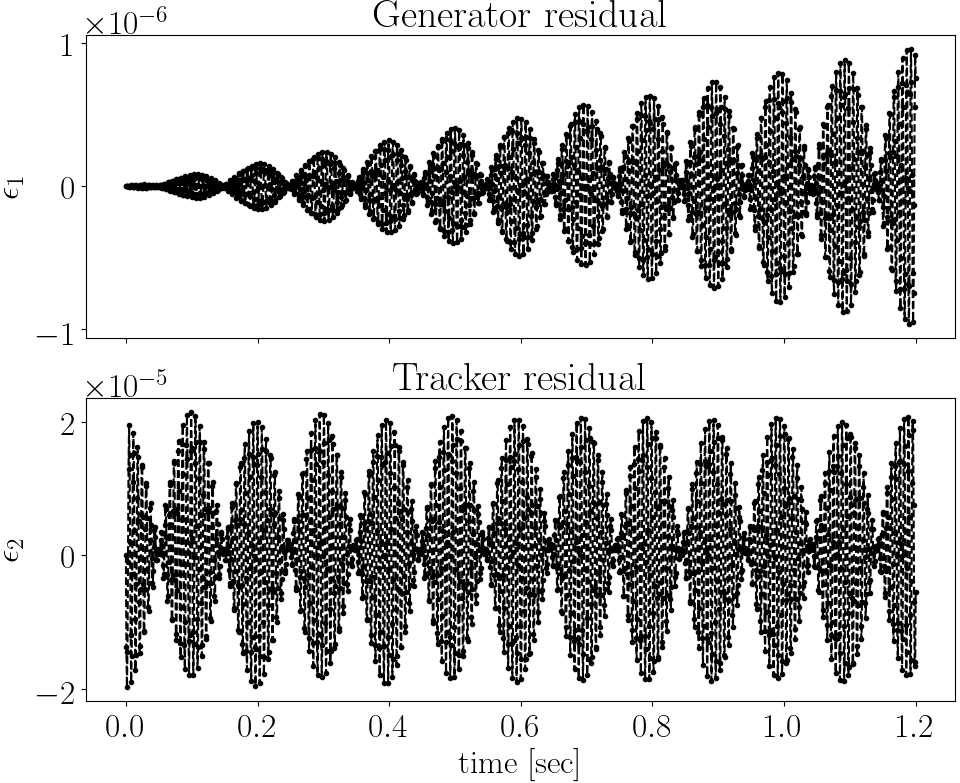
\includegraphics[height=.33\paperheight]{images/smp_sim/residual_vs_time(both)}
	\caption{Сравнительные невязки как функции времени.
		Верхняя панель: невязка $\epsilon_1$; нижняя панель: невязка $\epsilon_2$\label{fig:residuals}}
\end{figure}

На Рисунке~\ref{fig:sd:res} мы наблюдаем, что стандартные отклонения обеих невязок показывают 
такую же зависимость от скорости вращения колеса, как и $\nu_s$ (Рисунок~\ref{fig:sd:nbar}, нижняя панель),
 но не как стандартное отклонение компонент $\bar n$.
Это свидетельствует о том, что вариация частоты даёт значительно больший вклад в несоответствие между
моделью~\eqref{eq:fit_model} и трекерными данными, чем предполагаемая вариация амплитуды, вызванная изменением ориентации $\bar n$.

\begin{figure}[H]
	\centering
	\subbottom[Компонент $\bar n$\label{fig:sd:nbar}]{%
		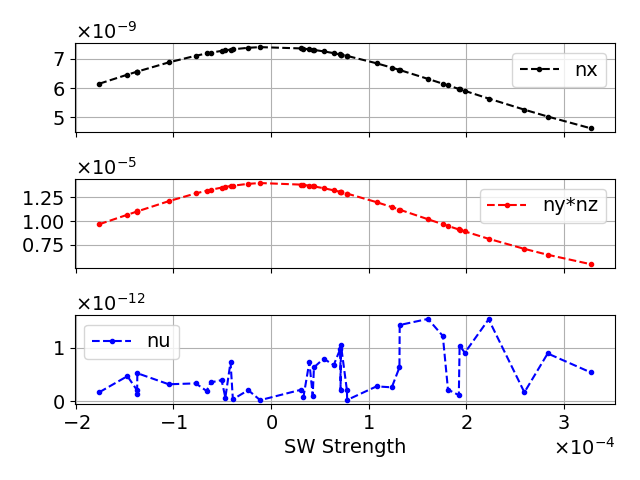
\includegraphics[height=.33\paperheight]{images/smp_sim/NBAR_variation_sd_vs_SW}}
	\subbottom[Сравнительных невязок.
	Верхняя панель: невязка $\epsilon_1$; нижняя панель: невязка $\epsilon_2$\label{fig:sd:res}]{%
		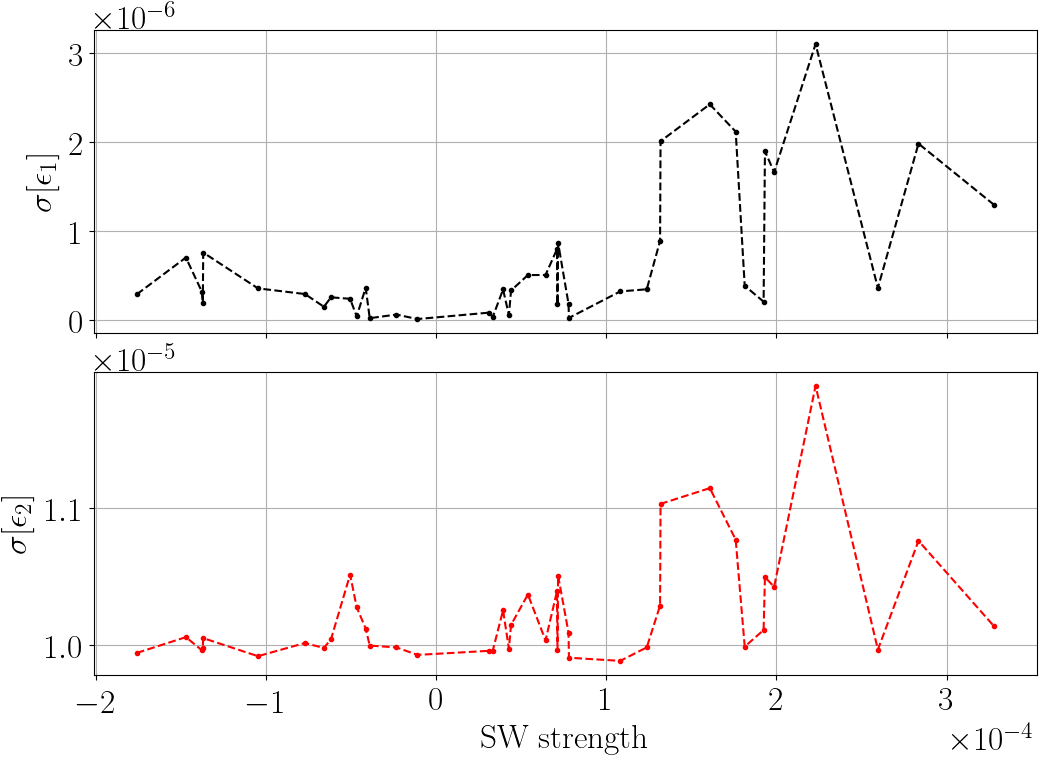
\includegraphics[height=.33\paperheight]{images/smp_sim/residual_SD_vs_SW(both)}}
	\caption{Стандартные отклонения в зависимости от относительной частоты МДМ спин-прецессии\label{fig:sd}}
\end{figure}

Таблица~\ref{tbl:param_estimates} характеризует качество фита модели по отношению к данным,
в случае самого медленного спин-колеса.
Видно, что попарные разницы между оценками параметров серий не являются статистически-значимыми. Хотя вариация вектора угловой скорости спин-прецессии ухудшила качество фита модели, она не ввела никакого статистически-значимого систематического смещения в оценки.

\begin{table}[h]\centering
	\caption{Оценки параметров модели (медленное спин-колесо)\label{tbl:param_estimates}}
	\begin{tabular}{r|rllr}
		\toprule
		Серия & Пар. & Величина & Ст.Ошибка & AIC \\
		\midrule
		\multirow{3}{*}{$s_y^{idl}$}
		& $\hat f$ & 4.220359687911 & $6.9\cdot10^{-11}$ & \multirow{3}{*}{-62093} \\
		& $\hat a$ & 0.12514597851 & $4\cdot10^{-11}$ & \\
		& $\hat\delta$ & $-1.50\cdot10^{-8}$ & $4\cdot 10^{-10}$ &\\
		\hline
		\multirow{3}{*}{$s_y^{gen}$}
		& $\hat f$ & 4.2203596911 & $1.9\cdot 10^{-9}$ & \multirow{3}{*}{-52142} \\
		& $\hat a$ & 0.125145979 & $1\cdot 10^{-9}$ & \\
		& $\hat\delta$ & $-1.6\cdot 10^{-8}$ & $1.2\cdot 10^{-8}$ &\\
		\hline
		\multirow{3}{*}{$s_y^{trk}$}
		& $\hat f$ & 4.2203603 & $1.3\cdot 10^{-6}$ & \multirow{3}{*}{-34567} \\
		& $\hat a$ & 0.12514597 & $3.7\cdot10^{-7}$ & \\
		& $\hat\delta$ & $-4\cdot10^{-6}$ & $6\cdot 10^{-6}$ &\\
		\bottomrule
	\end{tabular}
\end{table}

\subsection{Выводы}
Вопрос влияния бетатронного движения на ЭДМ статистику в FD-методологии следует рассматривать
ввиду трёх обстоятельств:
\begin{enumerate}
\item Осцилляции амплитуды сигнала очень малы. Они происходят на уровне не более $10^{-4}$ (при
  ${\alpha\sim N(0, 3\cdot 10^{-2})}$ градусов), тогда как ожидаемая неточность измерений поляризации находится
  на уровне процентов. Это значит, что суперпозиция систематической ошибки и случайной ошибки измерения
  не будет проявлять статистически-значимую систематичность.
\item Коэффициент корреляции между оценками амплитуды и частоты не значителен. Колебания амплитуды
  влияют на оценку $\hat a$ в первую очередь; их эффект на оценку $\hat\w$ опосредован, и описывается
  коэффициентом корреляции. Поскольку он меньше 10\%, даже если колебания окажутся достаточными, чтобы повлиять
  на оценку амплитуды, их эффект на оценку частоты будет уменьшен по крайней мере в 10 раз.
\item Этот систематический эффект контролируется. И этот фактор является основным достоинством методологий
  частотной области. Вводя в систему внешнее магнитное поле, колебания $\bar n$ могут быть 
  непрерывно минимизированы  до необходимого уровня, без каких-либо модификаций паттерна эксперимента.
\end{enumerate}


\section{Декогеренция спинов частиц пучка}\label{chpt3:decoherence}
Когеренцией спина называется мера или качество сохранения поляризации
в изначально полностью поляризованном пучке.~\cite[стр.~205]{Eremey:Thesis}

Когда поляризованный пучок инжектируется в накопительное кольцо, спин-векторы 
частиц пучка начинают прецессировать вокруг вертикального
(ведущего) поля. Частота прецессии зависит от равновесного уровня
энергии частицы, который различен для частиц пучка.

Это обстоятельство не является проблемой в том случае, когда начальная
поляризация пучка вертикальна; однако метод измерения ЭДМ в
накопительном кольце, основанный
на принципе замороженного спина \textbf{требует}, чтобы вектор поляризации
пучка был сонаправлен с его вектором импульса, т.е. лежал в
горизонтальной плоскости. Таким образом, декогеренция спина есть
внутренняя проблема метода замороженного спина.

В настоящем разделе мы исследуем причины возникновения спин-декогеренции,
метод борьбы с ней, а также приведём результаты симуляции, подтверждающей действенность
метода. Для начала, однако, определим время когеренции спина, требуемое для 
измерения ЭДМ методом замороженного кольца в пространственной области (space domain methodology).



\subsection{Требования к времени когеренции пучка}
Время когеренции спина (spin coherence time; SCT) для метода
замороженного спина, выполненного в накопительном кольце с идеально
установленными элементами определяется минимальным детектируемым углом
отклонения вектора поляризации пучка из горизонтальной плоскости
только засчёт ЭДМ. Для уровня чувствительности $10^{-29}~e\cdot cm$
это примерно $5\cdot10^{-6}$.~\cite{BNL:Deuteron2008}

В соответствии с уравнением Т-БМТ,
\[
\W_{EDM,x} = \eta\frac{qE_x}{2mc},
\]
где $\eta$ есть коэффициент пропорциональности между ЭДМ и спином,
равный $10^{-15}$ для дейтрона, для данного уровня чувствительности.~\cite[стр.~206]{Eremey:Thesis}

Для дейтронного BNL FS кольца, $E_x = 12$
МВ/м,~\cite[стр.~19]{BNL:Deuteron2008} так что $\W_{EDM,x}\approx
10^{-9}$ рад/сек. Таким образом получаем, что для того, чтобы достичь
детектируемый уровень отклонения вектора поляризации на 1 мкрад требуется SCT порядка 1000 секунд.~\cite[стр.~207]{Eremey:Thesis}
\subsection{Происхождение декогеренции}\label{sec:decoh:origin}
Декогеренция спина в пучке вызвана разницей угловых скоростей
прецессии спинов частиц, которая, в свою очередь, вызвана разницей
их длин орбит и импульсов. Влияние длины орбиты на спин-тюн частицы описывается 
понятием эффективного Лоренц-фактора, введённым в разделе~\ref{chpt1:FS-methods:effective-Lorentz-factor}.

Из уравнений~\eqref{eq:spin_tune_vs_gamma} для спин-тюна частицы в электромагнитном поле следует, 
что спин-тюны двух частиц с одинаковыми эффективными Лоренц-факторами равны, независимо от их траекторий в ускорителе. Этот принцип используется при использовании секступольных полей для подавления спиновой декогеренции, а также при смене полярности ведущего магнитного поля кольца.

\subsection{Теория секступольного подавления декогеренции}\label{sec:sextupole_spin_dec_solution}
Чтобы минимизировать декогеренцию спина, связанную с бетатронным
движением и отклонением импульса, могут быть использованы
секступольные (или октупольные) поля~\cite[стр.~212]{Eremey:Thesis}

Секступоль силы
\[
S_{sext} = \frac{1}{B\rho} \pddx{B_y}[x][2],
\]
где $B\rho$ магнитная жёсткость, влияет на коэффициент сжатия орбиты
первого порядка как~\cite[стр.~2581]{Senichev:IPAC13}
\begin{align}
	\Delta \alpha_{1,sext} &= -\frac{S_{sext}D_0^3}{L}, \label{eq:Sext_compaction_effect}
	\intertext{и одновременно на длину орбиты как}
	\bkt{\frac{\Delta L}{L}}_{sext} &= \mp \frac{S_{sext}D_0\beta_{x,y}\varepsilon_{x,y}}{L}, \label{eq:Sext_OL_effect}
\end{align}
где $D(s,\delta) = D_0(s) + D_1(s)\delta$ обозначает функцию дисперсии.

Принцип действия секступольного подавления декогеренции можно сформулировать следующим образом. Частица в ускорителе совершает бетатронные колебания вокруг замкнутой орбиты. Из-за дисперсии, замкнутая орбита отличается для разных частиц пучка. Секступоль работает как призма, фокусируя (либо дефокусируя) замкнутые орбиты различных частиц.

В следующих разделах мы будем называть декогеренцию, связанную с
горизонтальными/вертикальными бетатронными, и синхротронными
колебаниями соответственно X-/Y-, и D-декогеренцией. Семейства секступолей, 
подавляющие X-, Y-, и D-декогеренцию, будем обозначать соответственно GSX, GSY, GSD.

Из уравнений~\eqref{eq:Sext_compaction_effect}, и~\eqref{eq:Sext_OL_effect} можно
видеть, что для подавления декогеренции необходимы три семейства
секступолей, помещённых в максимумы функций: $\beta_x$, $\beta_y$ для подавления
X-,Y-декогеренции, и $D_0$ для D-декогеренции.

\subsection{Симуляция секступольного подавления декогеренции в идеальном ускорителе}\label{sec:decoh:suppression_in_ideal_lattice}

Мы провели симуляцию для проверки возможности подавления декогеренции секступольными полями. В симуляции 
была использована идеальная структура с замороженным спином, описанная в разделе~\ref{chpt2:lattice:FS_BNL}.
Поскольку элементы в структуре установлены идеально, спин-векторы частиц не поворачиваются вокруг радиальной
оси; прецессия происходит только в горизонтальной слоскости, вокруг вектора $\hat y$. 

Оптимизация производится на энергии пучка 270.00 МэВ, орбитальная и спиновая трансфер-матрицы структуры
вычисляются до пятого порядка разложения ряда Тэйлора.

В структуре используются три семейства секступолей, для подавления, соответственно, декогеренции связанной 
с горизонтальными, вертикальными бетатронными колебаниями, и с синхротронными колебаниями частиц.
Оптимальное значение градиента для каждого семейства отыскивается по-отдельности; значения полей двух
других семейств зануляются. Решение оптимизировать секступоли отдельно было принято потому, что
одновременная оптимизация всех трёх градиентов вела к численным проблемам в процедуре TSS.\footnote{Также,
мы изучали принципиальную возможность оптимизации всех трёх семейств секступолей, посредством прямого
вычисления необходимых коэффициентов разложения ряда Тэйлора на трёхмерной сетке значений градиентов. 
Вопрос требует более детального рассмотрения, но на данном этапе мы сомневаемся в принципиальной возможности
оптимизации всех трёх семейств секступолей. Возможно по этой причине в~\cite[стр.~219]{Eremey:Thesis} в BNL структуре
используется всего два семейства.}

В процессе оптимизации сначала вычисляются трансфер-матрицы структуры для заданного значения градиента, 
затем процедурой TSS вычисляются разложения Тэйлора спин-тюна и оси стабильного спина. В зависимости от 
оптимизируемого семейства, из разложения спин-тюна выбирается коэффициент при квадрате соответствующей
координаты фазового пространства ($x$, $y$, или $\delta$). Модуль коэффициента служит целевой функцией: т.е., 
при оптимальном значении градиента секступолей, спин-тюн не зависит (параболически) от соответствующего отклонения частицы от референсной.

При оптимизации используется алгоритм Simplex.~\cite[стр.~37]{COSYINF:Manual:Programmer}

На Рисунке~\ref{fig:decoh:perfect} изображены зависимости спин-тюна от смещения частицы от референсной по трём
координатам фазового пространства до и после включения оптимизированных секступолей. Можно наблюдать, что во 
всех трёх случаях удалось подавить параболическую зависимость спин-тюна от коордитаны. При этом сохраняется 
линейная зависимость, которая не чувствительна к секступольным полям. Линейная зависимость наблюдается при
моделировании ускорителя в коде COSY INFINITY, в коде MODE, а также при помощи программы MAD (из личной беседы
с проф. Сеничевым). Исходя из этого, можно предположить, что эффект не является численным артефактом COSY 
INFINITY, а имеет физическое обоснование. Этот вопрос требует дальнейшего рассмотрения, но на данный момент
считается, что он подавляется соответствующей подстройкой параметров ВЧ-резонатора.~\cite[стр.~210,~219]{Eremey:Thesis}

\begin{figure}[!h]
	\centering
	\subbottom[В горизонтальном направлении]{%
		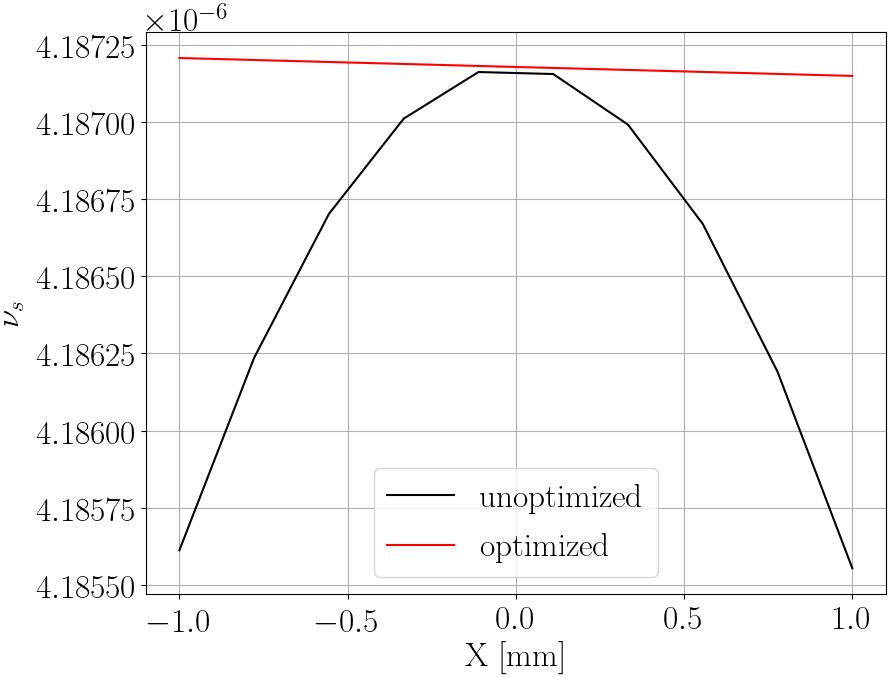
\includegraphics[height=.35\paperheight]{images/decoh_sim/spin_tune_decoh_x_offset}}
	\subbottom[В вертикальном направлении]{%
		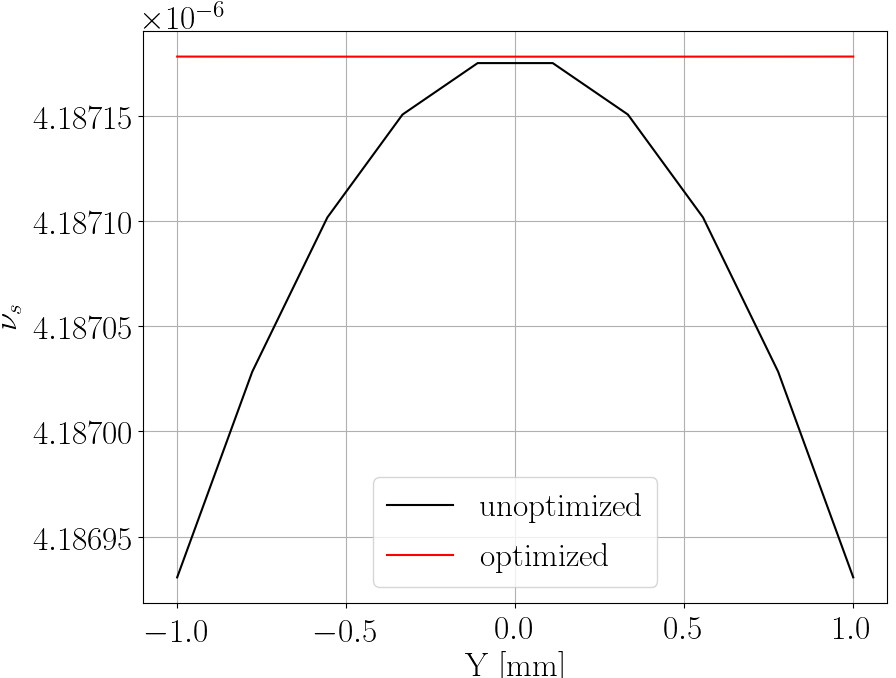
\includegraphics[height=.35\paperheight]{images/decoh_sim/spin_tune_decoh_y_offset}}
\end{figure}
\begin{figure}[!h]\centering
	\contsubbottom[По энергии]{%
		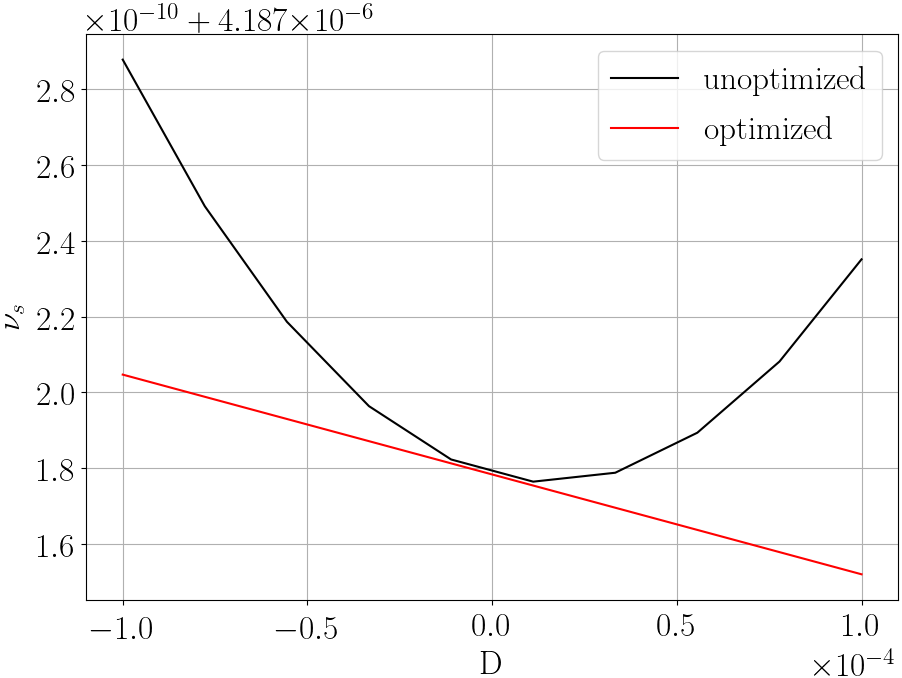
\includegraphics[height=.35\paperheight]{images/decoh_sim/spin_tune_decoh_d_offset}}
	\legend{Цветом выделены зависимости при нулевом (чёрный) и оптимизированном (красный) значениях градиента секступоля}
	\caption{Зависимость спин-тюна частицы от её смещения от референсной частицы.\label{fig:decoh:perfect}}
\end{figure}

\subsection{Переход декогеренции из горизонтальной плоскости в вертикальную, при появлении неидеальностей}
В неидеальную структуру с замороженным спином инжектировался ансамбль из 30 частиц, равномерно смещённых 
от референсной в вертикальном направлении в диапазоне $y \in [-1, +1]$ мм. Поскольку анализ производится только
на основании данных трекинга, пучок инжектирован на кинетической энергии строго замороженного спина
270.0092 МэВ.

Неидеальности структуры моделируются наклонами E+B элементов вокруг оптической оси на углы, 
взятые из нормального распределения $\Theta_{tilt} \sim N(0, 1\cdot 10^{-4})$ радиан. 
Поскольку при введении таких неидеальностий сохраняется величина силы Лоренца, они не искажают 
орбитальную динамику частицы, и отражаются только на спиновой динамике. Величина стандартного отклонения
отражает реалистичную неточность установки элементов ускорителя. 

На Рисунке~\ref{fig:decoh:SX_SD} представлено стандартное отклонение радиальных компонент спин-векторов ансамбля
до и после включения секступолей. Поскольку частицы движутся в неидеальной структуре, их спин-векторы вращаются
в вертикальной плоскости с большой скоростью, и потому $\sigma_{s_x}$ --- быстро-осциллирующая функция, не
показывающая долгосрочной тенденции к росту (наклон прямой $(2\pm2)\cdot 10^{-8}$ 1/сек). Таким образом, 
не наблюдается декогеренции спина в горизонтальной плоскости. При использовании секступолей 
амплитуда колебаний $\sigma_{s_x}$ уменьшается на порядок.

На Рисунке~\ref{fig:decoh:SY_SD} представлена та же статистика  для вертикальных компонент спин-векторов. Наблюдается долгосрочный тренд, 
(наклон $(4.5 \pm 0.6)\cdot 10^{-7}$ 1/сек) до включения корректирующих секступолей. Секступольная коррекция не уменьшает амплитуду колебаний, 
но подавляет тренд (наклон после включения секступолей $(5\pm 6)\cdot 10^{-8}$ 1/сек).

\begin{figure}[h!]
	\centering
	\subbottom[Без секступолей]{%
		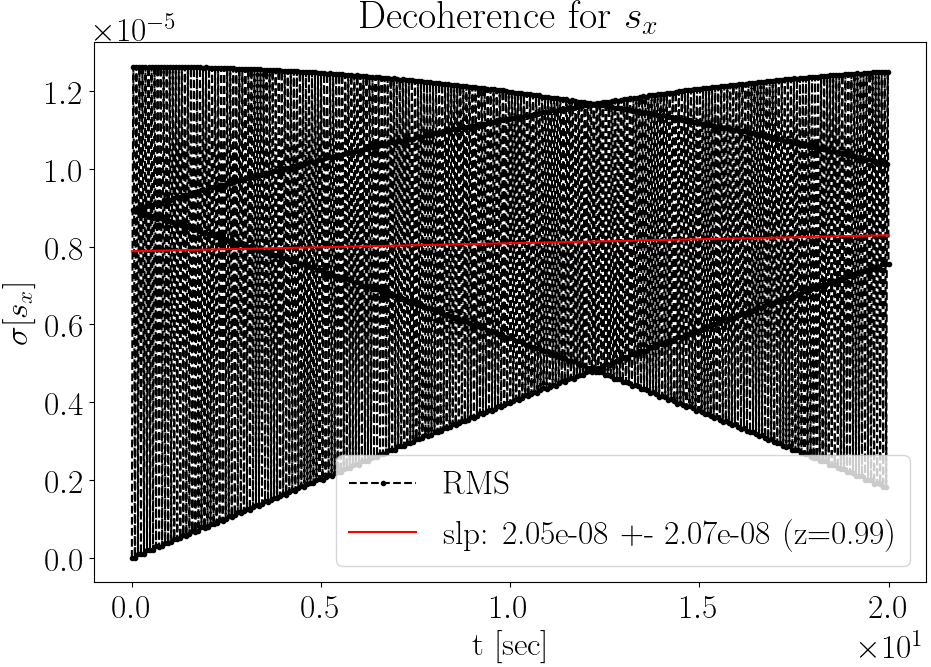
\includegraphics[height=.35\paperheight]{images/decoh_sim/SX_decoh_20sec_unopt}}
	\subbottom[С секступолями]{%
		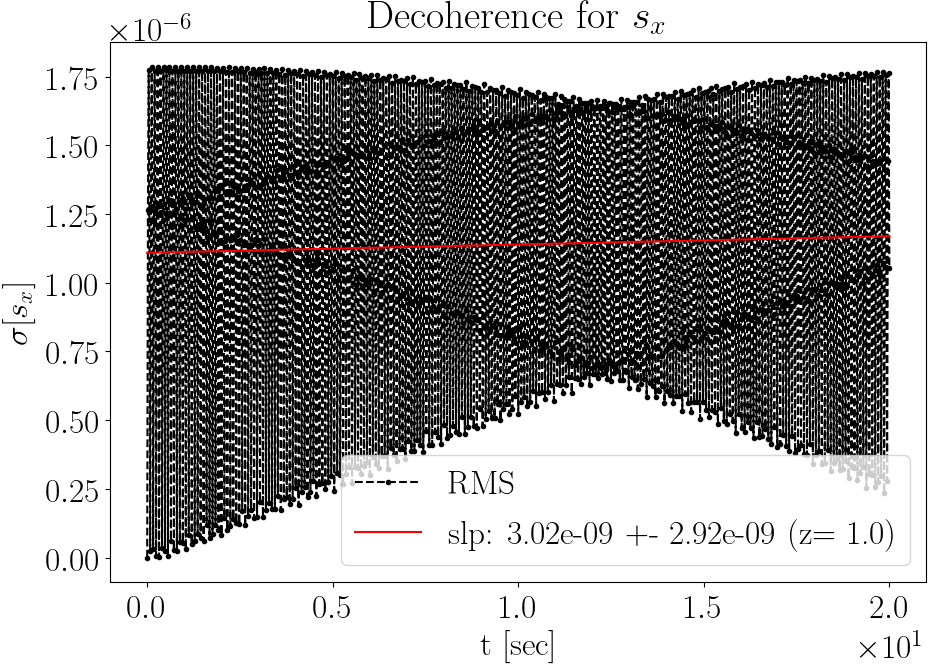
\includegraphics[height=.35\paperheight]{images/decoh_sim/SX_decoh_20sec_opt}}
	\caption{Стандартное отклонение радиальной компоненты спин-вектора частицы от спин-вектора референсной частицы\label{fig:decoh:SX_SD}}
\end{figure}

\begin{figure}[h!]
	\centering
	\subbottom[Без секступолей]{%
		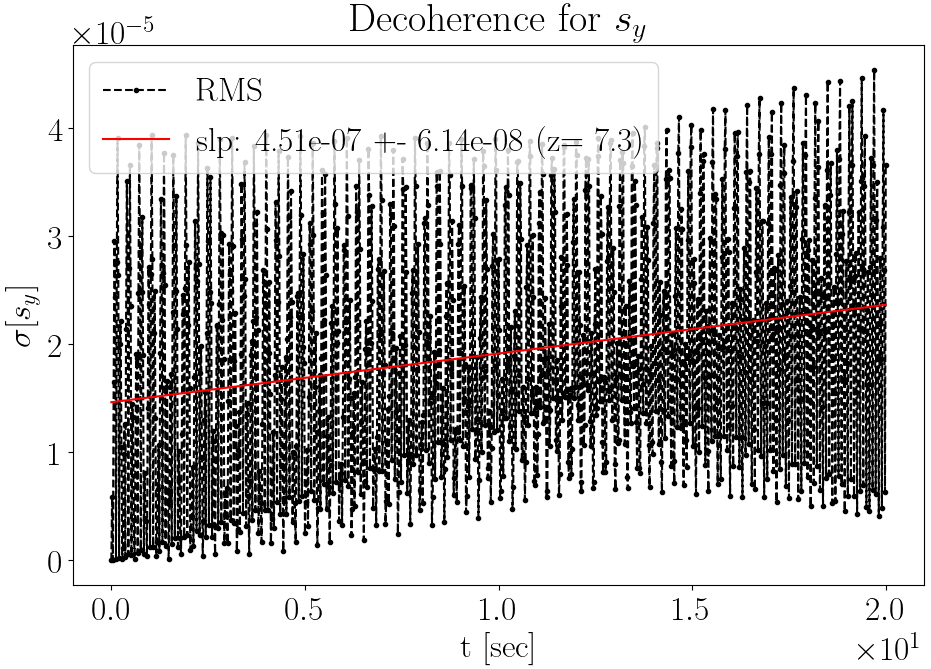
\includegraphics[height=.35\paperheight]{images/decoh_sim/SY_decoh_20sec_unopt}}
	\subbottom[С секступолями]{%
		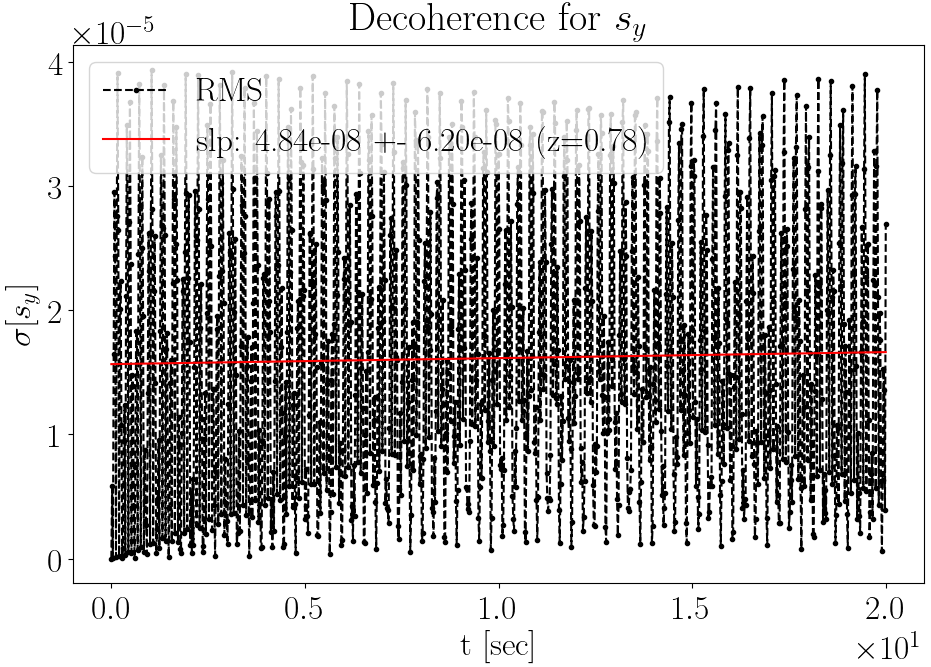
\includegraphics[height=.35\paperheight]{images/decoh_sim/SY_decoh_20sec_opt}}
	\caption{Стандартное отклонение вертикальной компоненты спин-вектора частицы от спин-вектора референсной частицы\label{fig:decoh:SY_SD}}
\end{figure}

\subsection{Симуляция эксперимента по подавлению декогеренции  в неидеальном ускорителе}\label{sec:decoh:sim-imperfect}
При проведении нижеследующих тестов симулировалась инжекция
плоского, гауссовского пучка в структуру с замороженным
спином. E+B спин-ротаторы в структуре были установлены со случайно распределённым углом наклона вокруг оптической оси, взятым из распределения $N(0, 5\cdot10^{-4})$ радиан.

Инжектируемые пучки состояли из 30 частиц, распределённых в вертикальной
плоскости $y-z$ как $y\sim N(y_0, 0.1)$ мм; все остальные координаты равны нулю.
Оффсет $y_0$ варьировался в диапазоне $[-1, +1]$ мм. Начальное
направление спин-векторов всех частиц --- продольное: $\vec S(t=0) = (0,0,1)$.

Также в структуре варьировалось значение градиента $G_Y$ секступоля,
модулирующего декогеренцию в вертикальной плоскости. $G_Y$ менялся в
диапазоне $[G_Y^0 - 5\cdot10^{-3}, G_Y^0 + 5\cdot10^{-3}]$, где
$G_Y^0=-5.77\cdot 10^{-4}$ --- оптимальное значение градиента для заданных 
неидеальностей структуры. Величина $G_Y^0$ была найдена путём минимизации коэффициента разложения $a_2$
ряда Тэйлора $\nu_s(y) \approx a_0 + a_1\cdot y + a_2\cdot y^2 + O(y^3)$.

На каждое значение градиента приходится 10 инжекций.

Для того, чтобы обеспечить устойчивость процедуры TSS COSY Infinity~\cite{COSYINF:Manual:BeamPhys}, пучок инжектировался на энергии 270 МэВ (строгий FS находится на энергии 270.0092 МэВ), а матрицы перехода орбитального и спинового движений строились до третьего порядка разложения ряда Тэйлора. 

Далее ансамбль начальных значений, представляющий пучок, трекается
через структуру на протяжении $1.2\cdot10^6$ оборотов, что
примерно эквивалентно 1.2 секундам. Каждые 800 оборотов производится
запись необходимых для анализа данных.

Собираемые данные: 
\begin{enumerate*}[\itshape a\upshape)]
	\item результаты вычислений процедуры TSS: спин-тюн $\nu_s$ и компоненты вектора оси инвариантного спина $\bar n$, и
	\item компоненты спина $(S_X, S_Y, S_Z)$, и фазового пространства $(X,A,Y,B,T,D)$.
\end{enumerate*}
Мы также записывали разложения ряда Тэйлора функций $\nu_s$, $\nbar$, орбитальной, и спиновой трансфер матриц
структур для каждого значения $G_Y$.

Из данных по компонентам спина вычисляется вектор поляризации банча:
\begin{equation}\label{eq:polarization_formula}
\vec P = \frac{\sum_i\vec s_i}{|\sum_i\vec s_i|}.
\end{equation}

Вертикальная компонента вектора фиритуется функцией $f(t; a,f,\phi) = a\cdot \sin(2\pi\cdot
f\cdot t + \phi)$, оцениваются все три параметра $(\hat a, \hat f,
\hat\phi)$. 

\subsubsection{Эффект секступольных полей на спин-тюн и на ось стабильного спина}
На Рисунке~\ref{decoh:fig:ST_vs_y0_GSY} представлена зависимость спин-тюна от вертикального смещения частицы от референсной орбиты: $\nu_s(y) \approx a_0 + a_1\cdot y + a_2\cdot y^2 + O(y^3)$. На Рисунке~\ref{decoh:fig:full:ST_vs_y0_GSY} можно наблюдать разгибание ветвей параболы при $G_Y \rightarrow G_Y^0$.
\begin{figure}[h!]
	\centering
	\subbottom[Полный диапазон~\label{decoh:fig:full:ST_vs_y0_GSY}]{%
		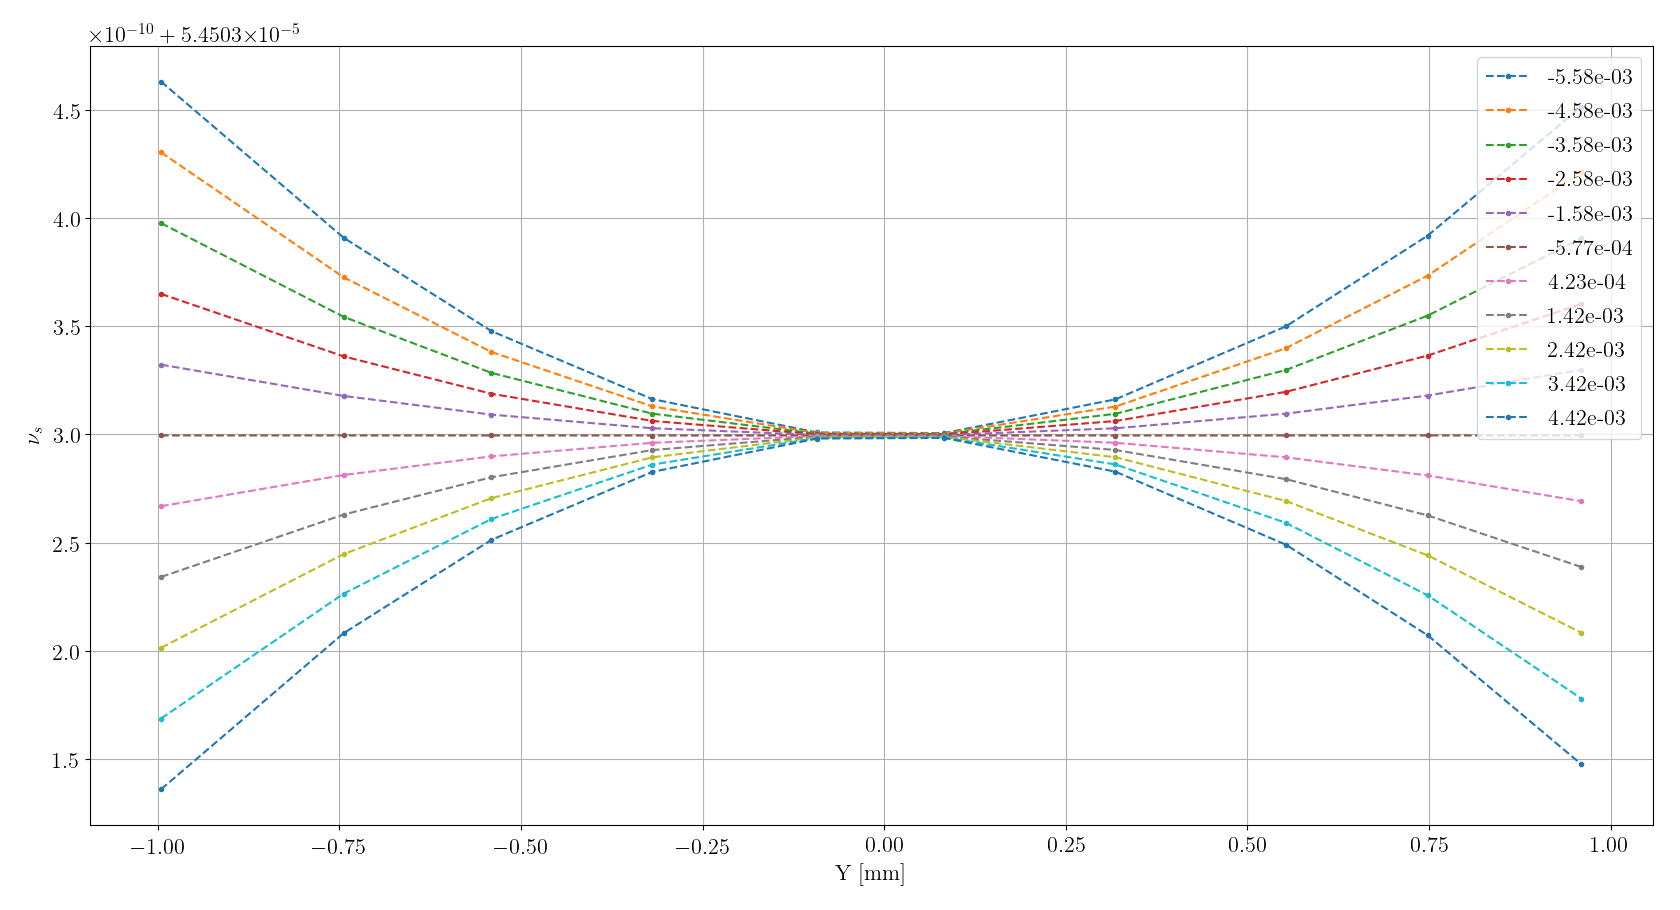
\includegraphics[width=\linewidth]{images/decoh_sim/spin_tune_vs_offset}}
	\subbottom[Деталировка кривой при оптимальном значении $G_Y$\label{decoh:fig:zoom:ST_vs_y0_GSY}]{%
		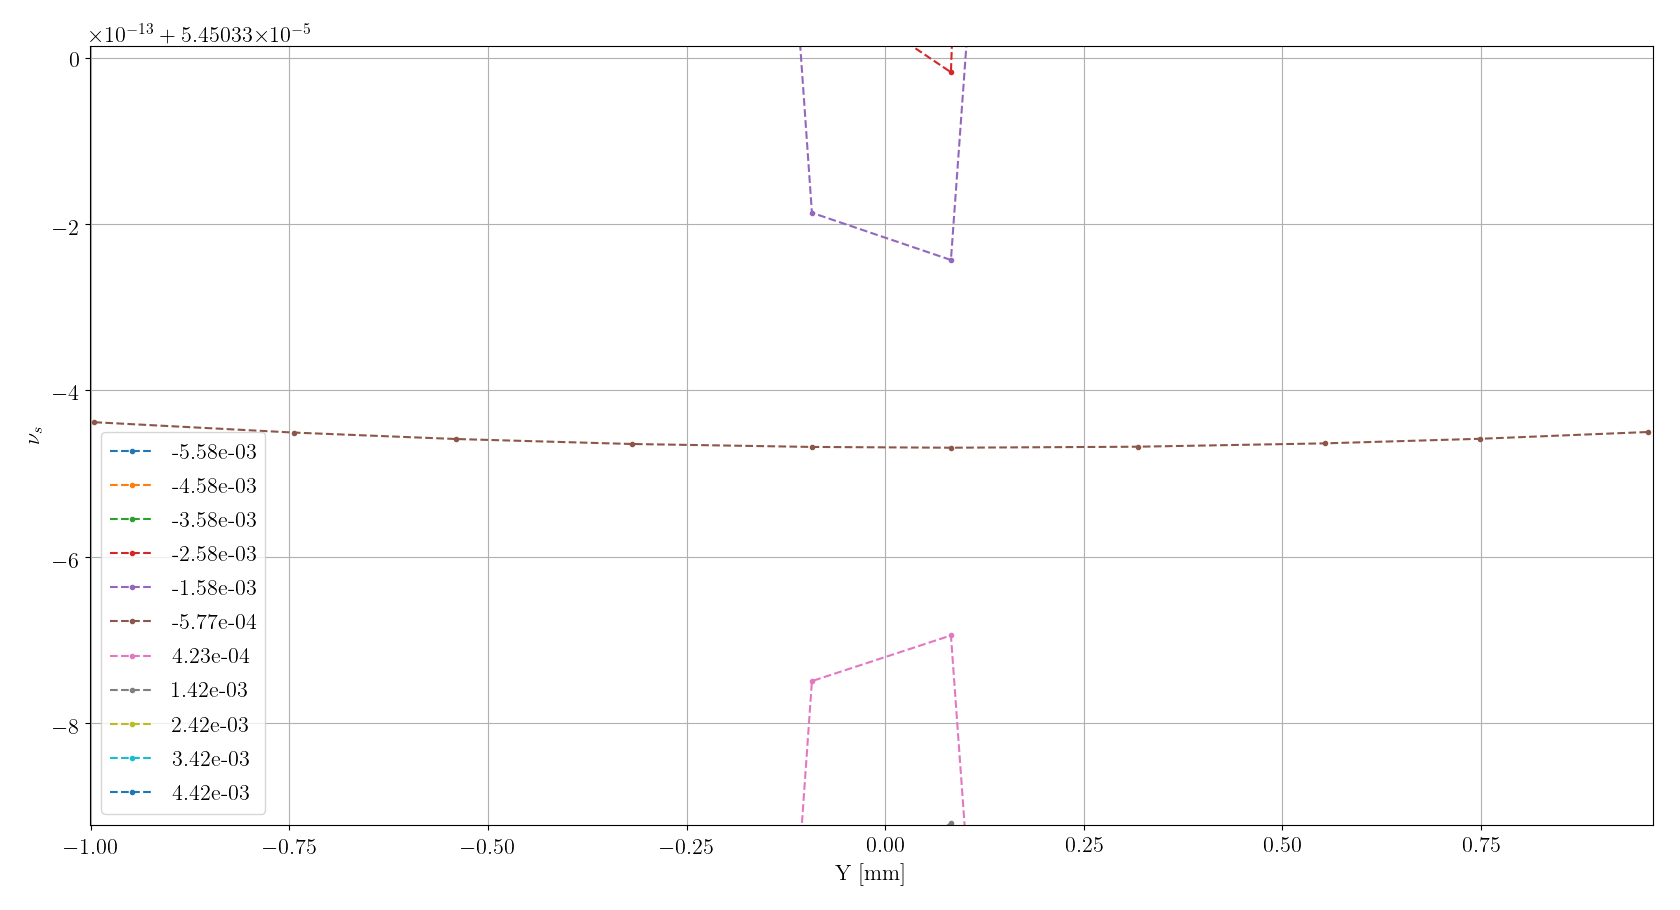
\includegraphics[width=\linewidth]{images/decoh_sim/spin_tune_vs_offset_zoom}
	}
	\legend{Цветом обозначены данные для различных значений градиента $G_Y$ Y-секступоля.}
	\caption{Спин-тюн $\nu_s$ в зависимости от смещения частицы от референсной орбиты.\label{decoh:fig:ST_vs_y0_GSY}}
\end{figure}

Аналогичная зависимость для вертикальной компоненты оси стабильного спина частицы представлена на Рисунке~\ref{decoh:fig:ny_vs_y0_GSY}. На Рисунке~\ref{decoh:fig:full:ny_vs_y0_GSY} мы обнаруживаем, что компонента оси стабильного спина ведёт себя аналогично спин-тюну при $G_Y \rightarrow G_Y^0$. Как и в случае идеальной структуры, на Рисунке~\ref{decoh:fig:zoom:ny_vs_y0_GSY} наблюдается присутствие в разложении $\nbar_y(y)$ линейного члена, не чувствительного к секступольным полям.

\begin{figure}[h!]
	\centering
	\subbottom[Полный диапазон.\label{decoh:fig:full:ny_vs_y0_GSY}]{%
		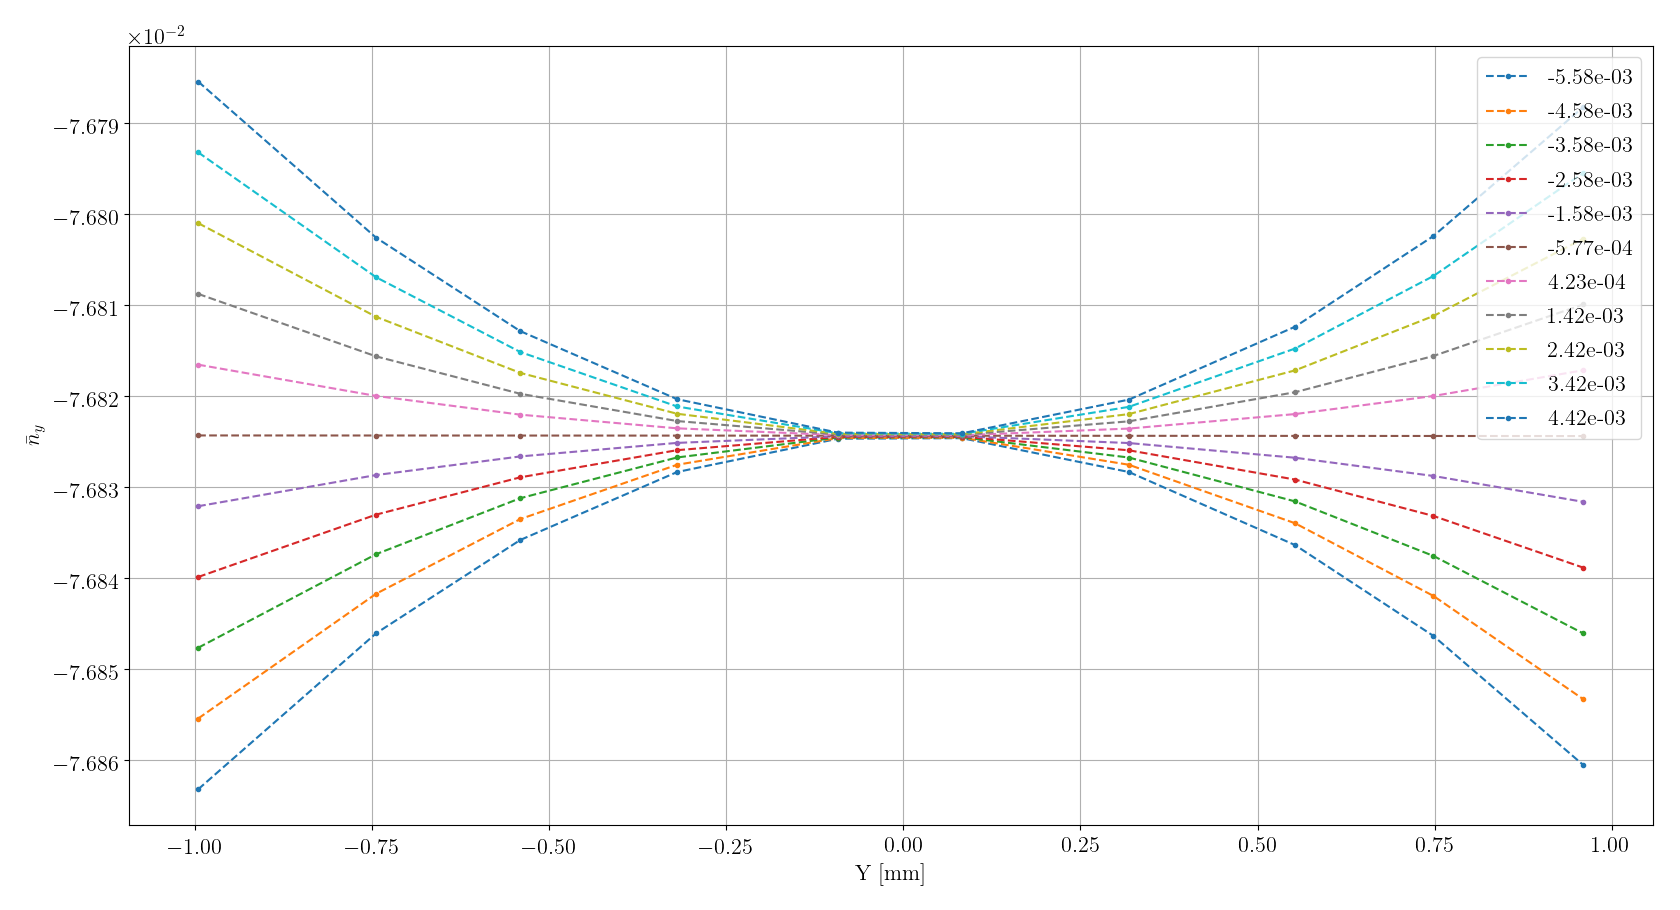
\includegraphics[width=\linewidth]{images/decoh_sim/ny_vs_offset}}
	\subbottom[Деталировка кривой при оптимальном значении $G_Y$.\label{decoh:fig:zoom:ny_vs_y0_GSY}]{%
		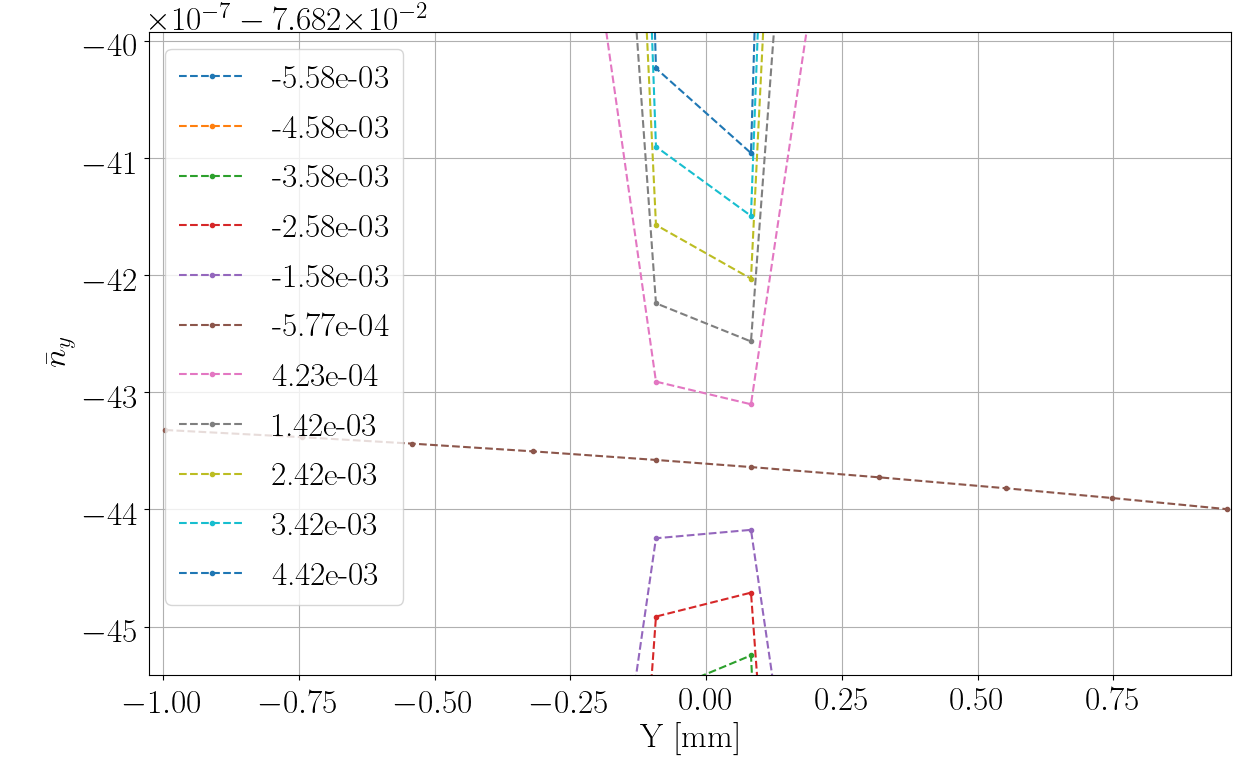
\includegraphics[width=\linewidth]{images/decoh_sim/ny_vs_offset_zoom}}
	\legend{Цветом обозначены данные для различных значений градиента $G_Y$ Y-секступоля.}
	\caption{Вертикальная компонента $\bar n_y$ оси прецессии спина в зависимости от смещения частицы от референсной орбиты.\label{decoh:fig:ny_vs_y0_GSY}}
\end{figure}

На рисунках выше, значения спин-тюна и компонент оси стабильного спина были вычислены как функции только одной переменной; все остальные координаты фазового пространства приняты равными нулю. Анализируя трекинговые данные, мы обнаружили, что компоненты оси стабильного спина (как впрочем и спин-тюн) частицы практически не варьируются, как можно было бы ожидать исходя из рисунков, а находятся на практически постоянном уровне. Мы предположили, что зависимости $\nu_s$ и $\nbar$ от вертикальной координаты и от её производной ($y'\equiv a$) компенсируют друг друга во время движения частицы по реальной тракетории. На следующих рисунках мы изобразили значения функций $\nu_s$, $\nbar$ на истинных траекториях частиц в ускорителе.

На Рисунке~\ref{decoh:fig:yb_traj} изображены траектории частиц в плоскости $(Y,B)$ фазового пространства, полученные в результате трекинга через неидеальный ускоритель.
\begin{figure}[h!]
	\centering
	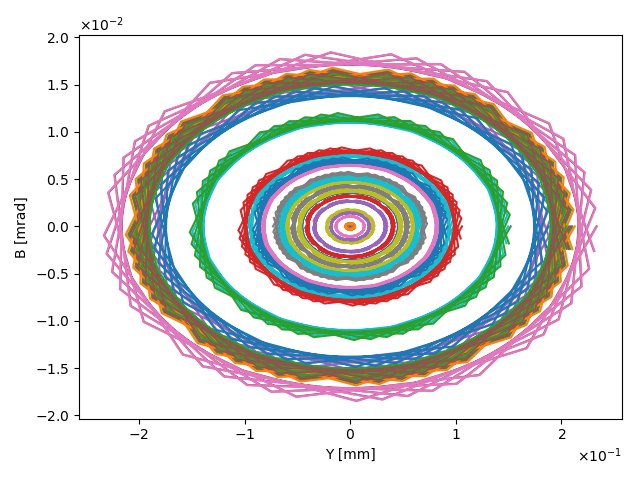
\includegraphics[width=\linewidth]{images/decoh_sim/YB-PHASE_SPACE_IMPERFECT_UNOPT}
	\caption{Траектории частиц в плоскости $(Y,B)$ фазового пространства.\label{decoh:fig:yb_traj}} 
\end{figure}

На Рисунках~\ref{decoh:fig:ST_on_traj}, \ref{decoh:fig:NX_on_traj}, \ref{decoh:fig:NY_on_traj}, и \ref{decoh:fig:NZ_on_traj} изображены, соответственно: спин-тюн, радиальная, вертикальная, и продольная компоненты оси прецессии спина, вычисленные на траекториях частиц из Рисунка~\ref{decoh:fig:yb_traj}, в двух случаях:
\begin{enumerate*}[\itshape i\upshape)]
	\item с выключенными, и 
	\item с включенными секступолями $G_Y$.
\end{enumerate*}  

\begin{figure}[!h]
	\centering
	\subbottom[С выключенными секступолями.]{%
		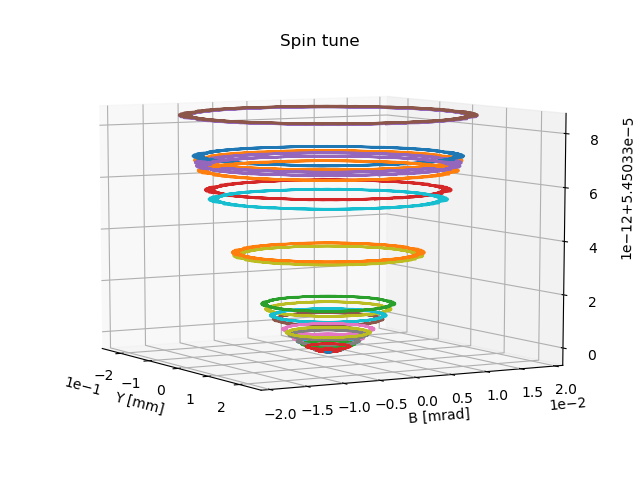
\includegraphics[width=\linewidth]{images/decoh_sim/ST_VS_YB_IMPERFECT_UNOPT}}
	\hfill
	\subbottom[С включенными секступолями.]{%
		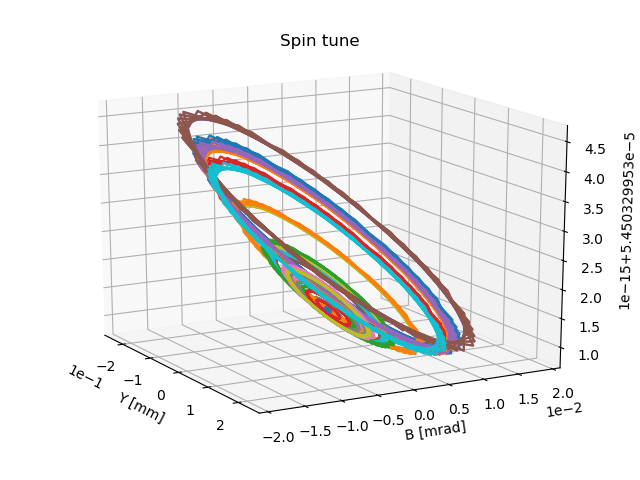
\includegraphics[width=\linewidth]{images/decoh_sim/ST_VS_YB_IMPERFECT_OPTIM}}
	\hfill
	\caption{Спин-тюны частиц на их траекториях в неидеальной FS-труктуре.\label{decoh:fig:ST_on_traj}}
\end{figure}

\begin{figure}[!h]
	\centering
	\subbottom[С выключенными секступолями.]{%
		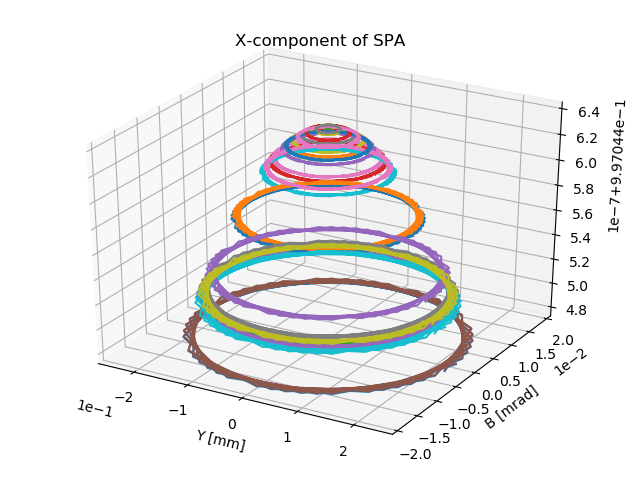
\includegraphics[width=\linewidth]{images/decoh_sim/NX_VS_YB_IMPERFECT_UNOPT}}
	\hfill
	\subbottom[С включенными секступолями.]{%
		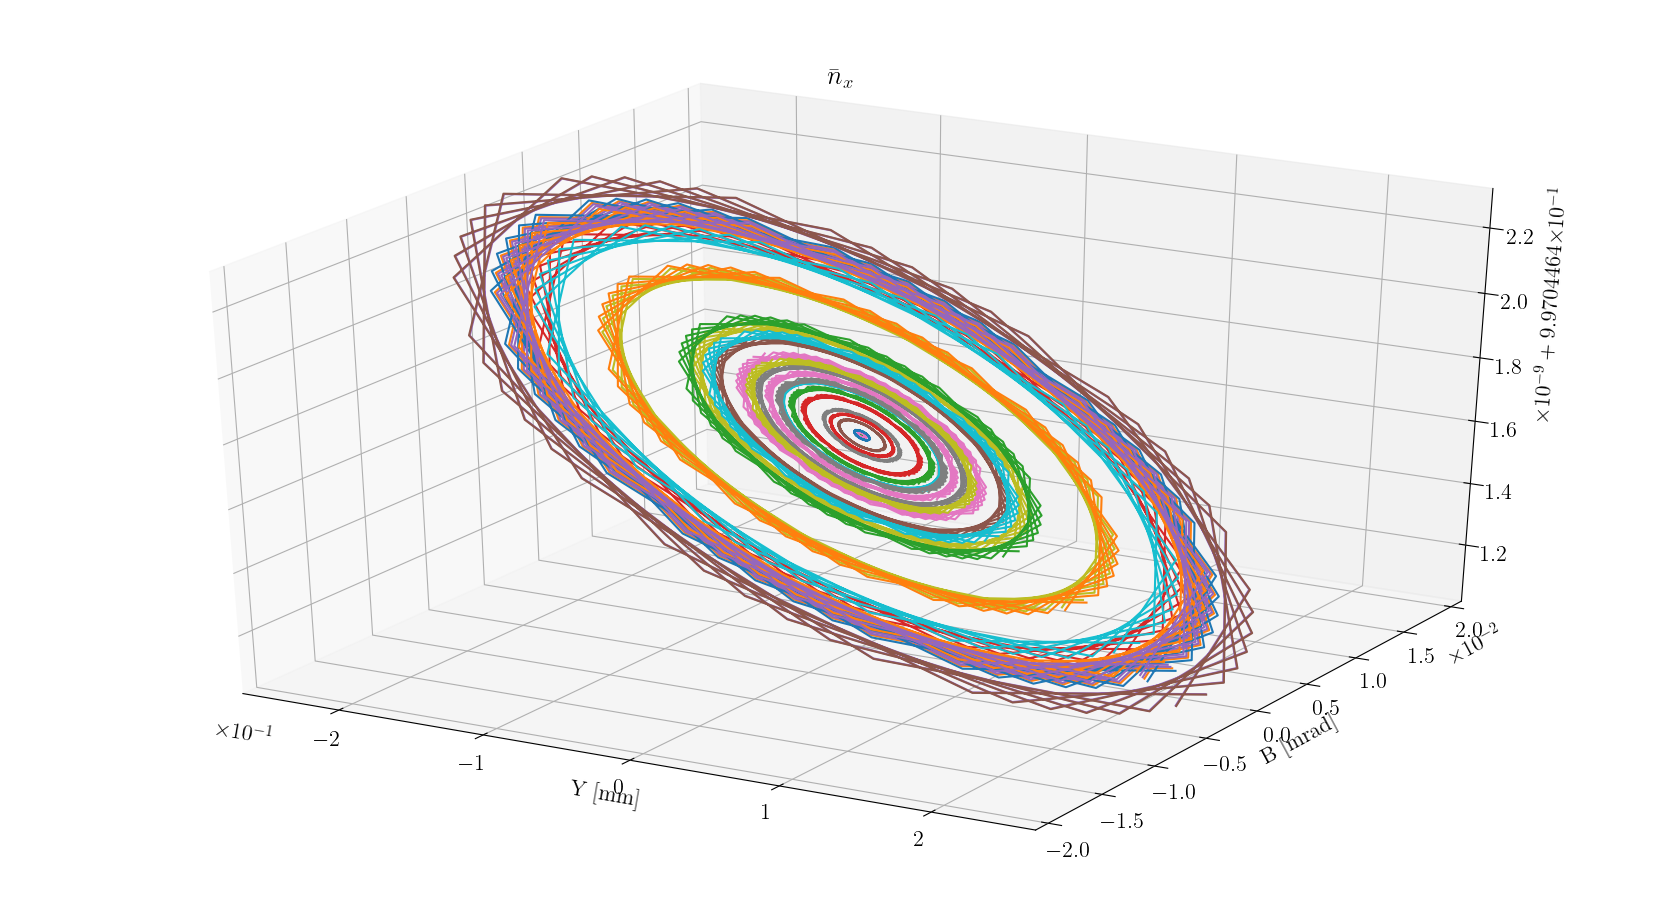
\includegraphics[width=\linewidth]{images/decoh_sim/NX_VS_YB_IMPERFECT_OPTIM}}
	\hfill
	\caption{Радиальные компоненты осей прецессии спинов частиц на их траекториях в неидеальной FS-труктуре.\label{decoh:fig:NX_on_traj}}
\end{figure}

\begin{figure}[!h]
	\centering
	\subbottom[С выключенными секступолями.]{%
		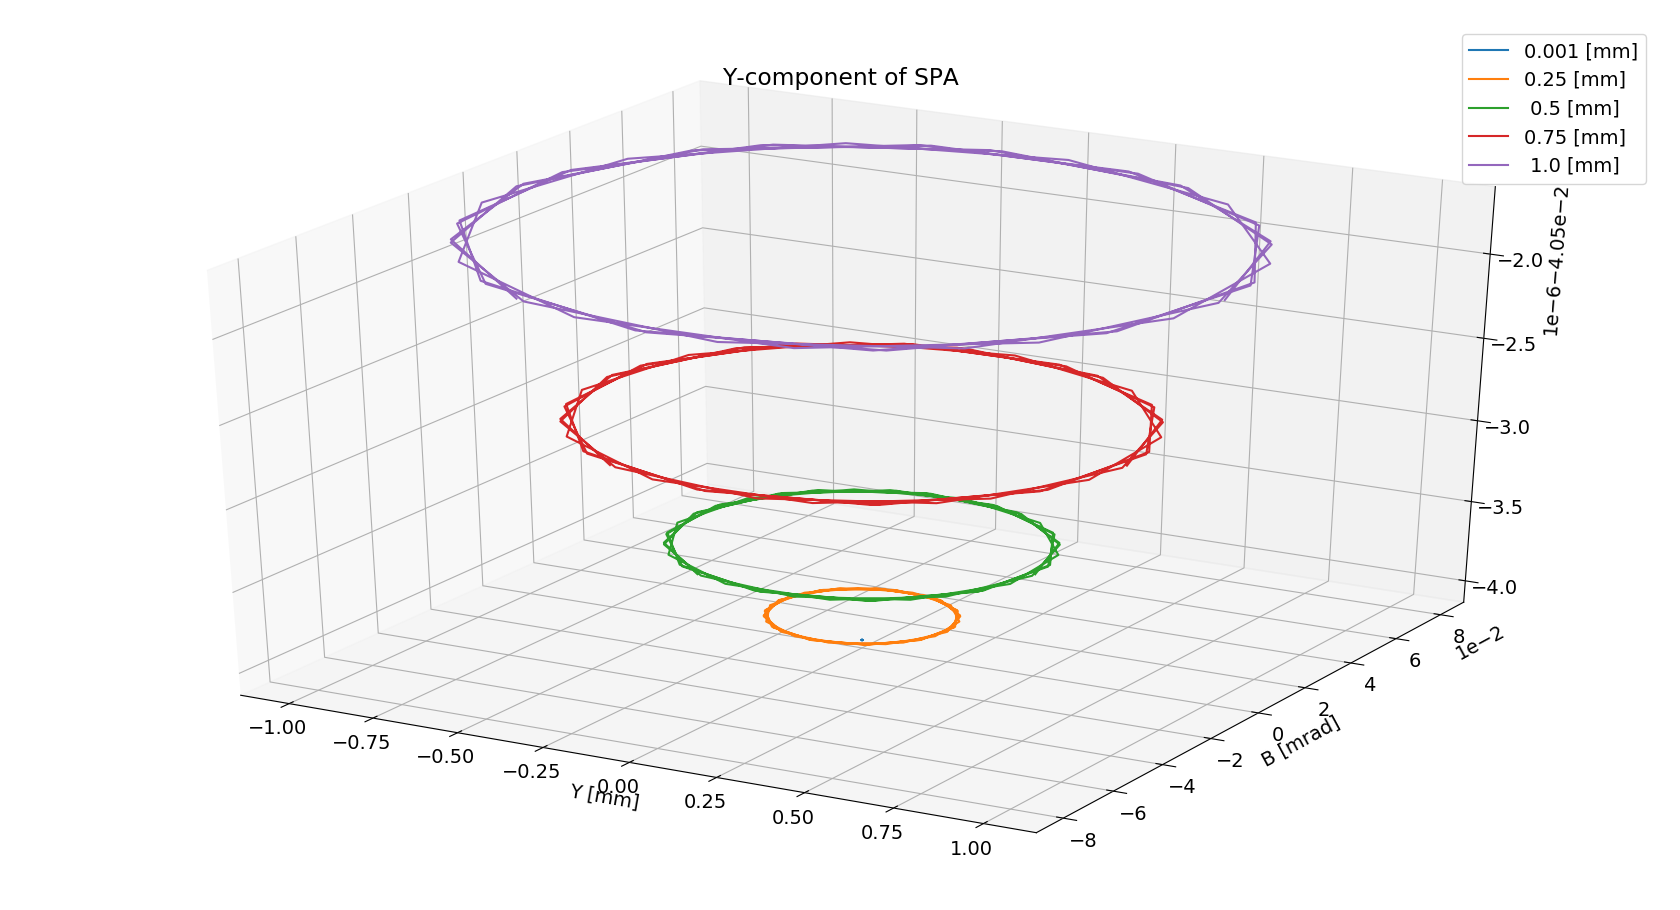
\includegraphics[width=\linewidth]{images/decoh_sim/NY_VS_YB_IMPERFECT_UNOPT}}
	\hfill
	\subbottom[С включенными секступолями.]{%
		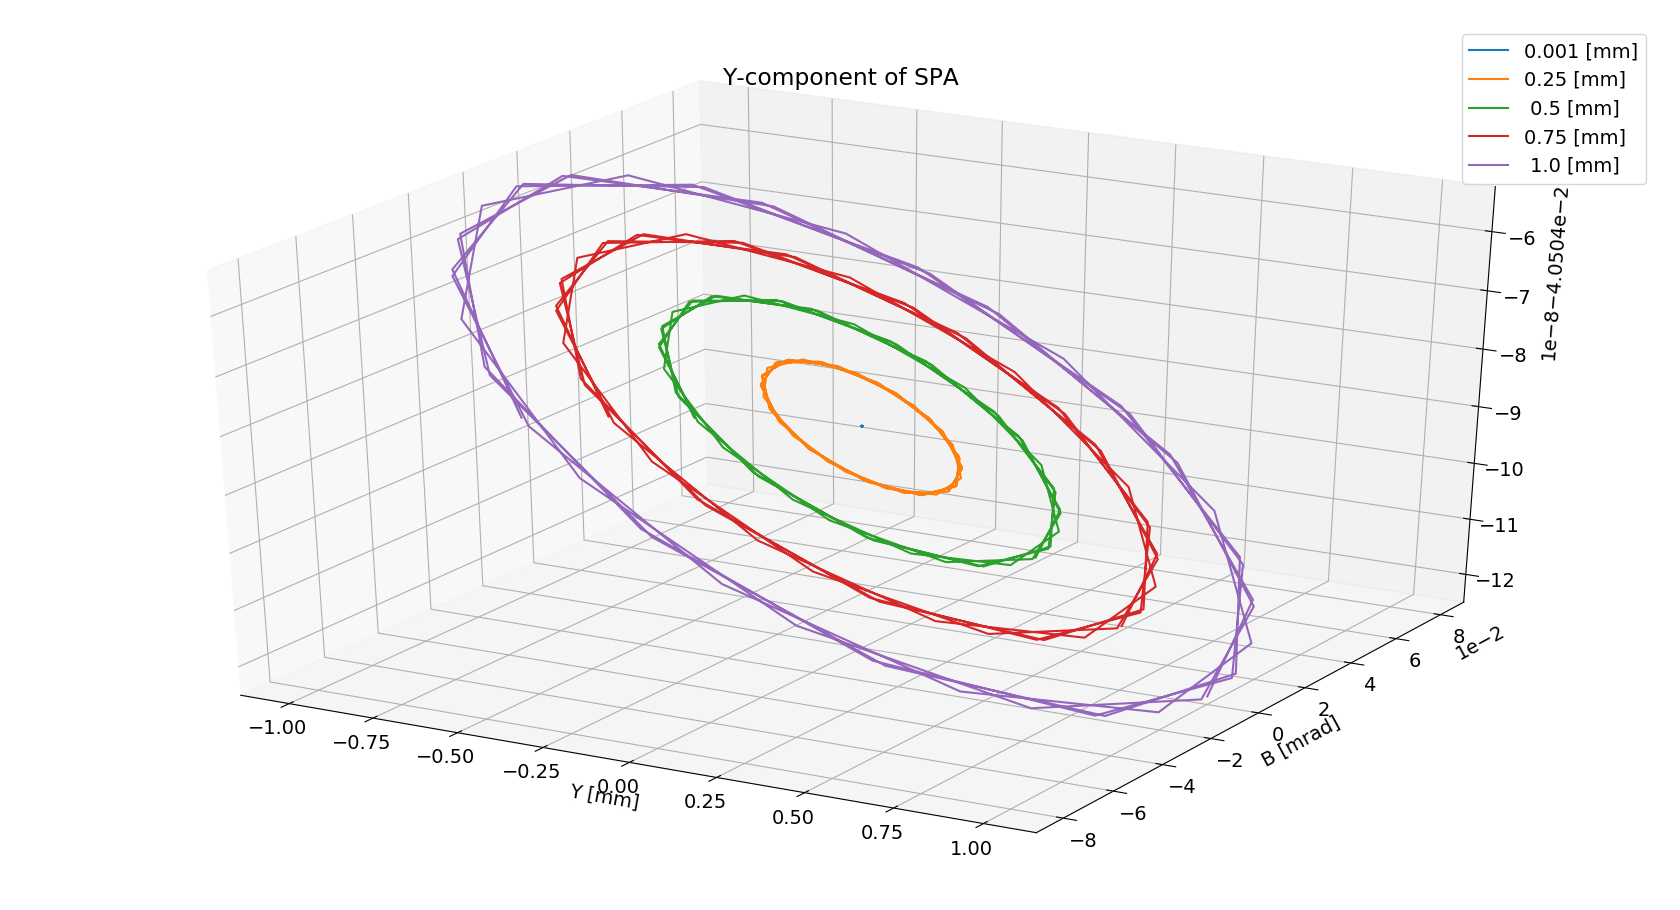
\includegraphics[width=\linewidth]{images/decoh_sim/NY_VS_YB_IMPERFECT_OPTIM}}
	\hfill
	\caption{Вертикальные компоненты осей прецессии спинов частиц на их траекториях в неидеальной FS-труктуре.\label{decoh:fig:NY_on_traj}}
\end{figure}

\begin{figure}[!h]
	\centering
	\subbottom[С выключенными секступолями.]{%
		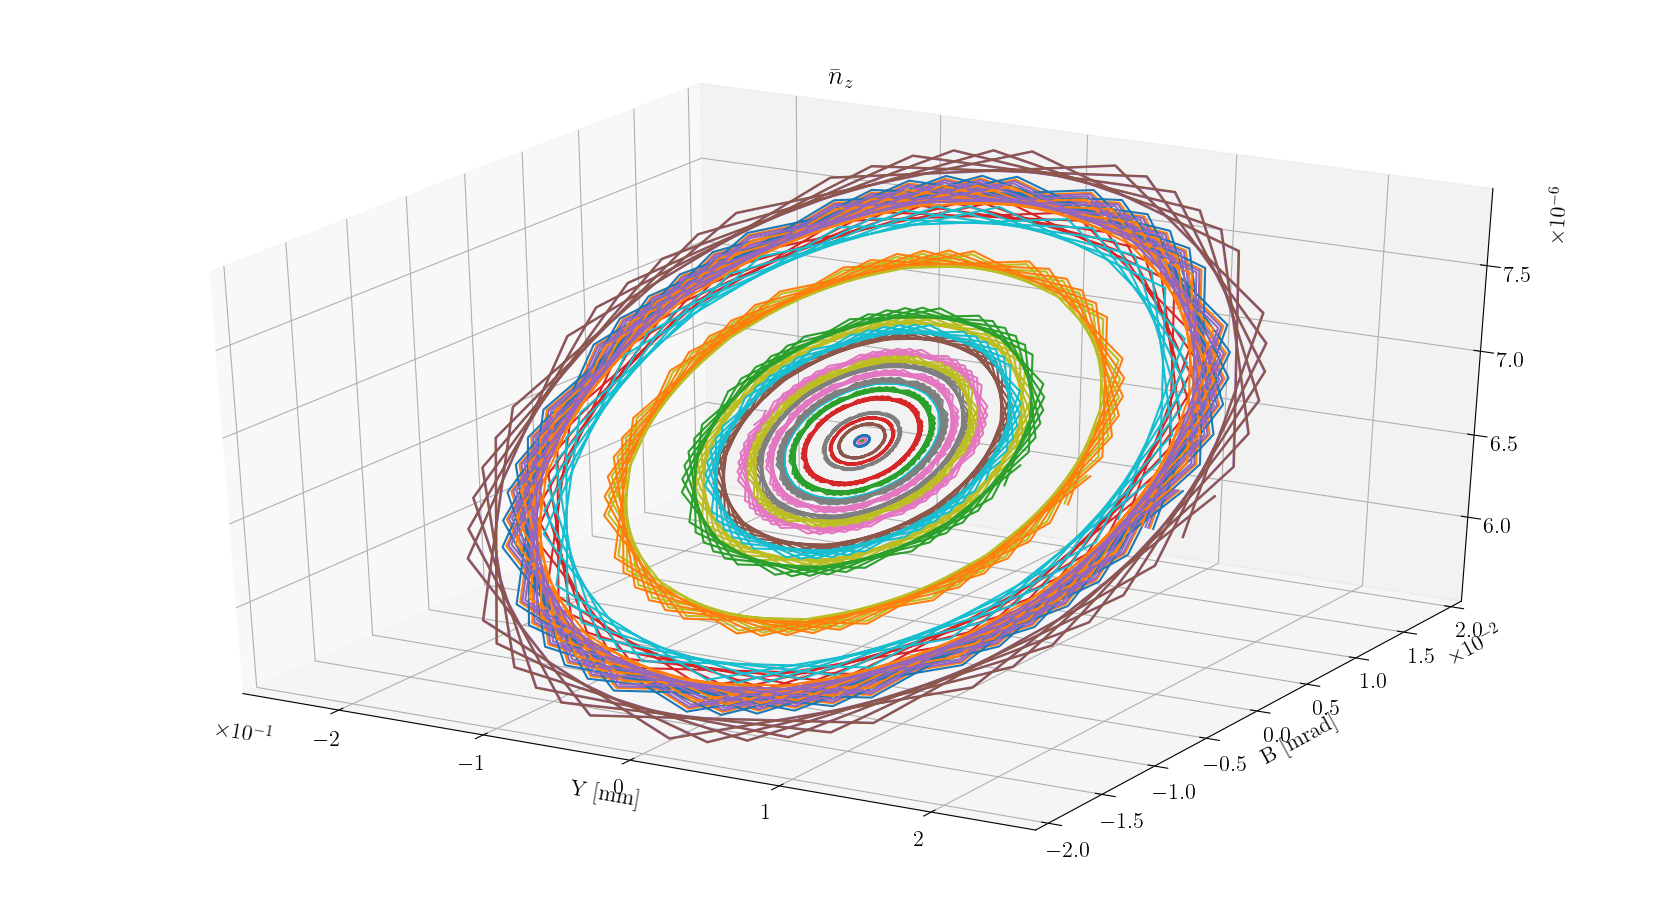
\includegraphics[width=\linewidth]{images/decoh_sim/NZ_VS_YB_IMPERFECT_UNOPT}}
	\hfill
	\subbottom[С включенными секступолями.]{%
		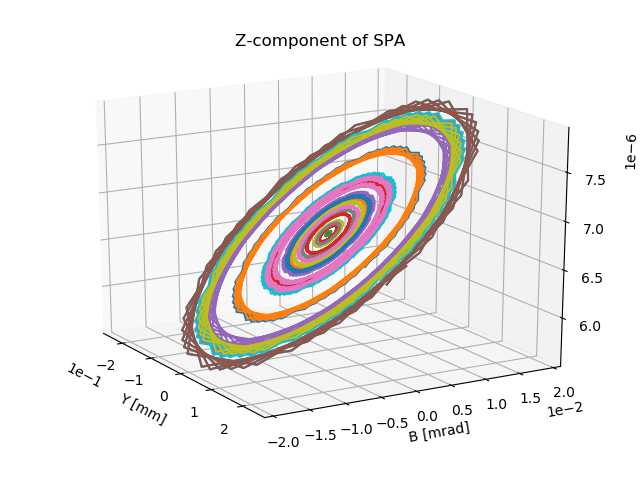
\includegraphics[width=\linewidth]{images/decoh_sim/NZ_VS_YB_IMPERFECT_OPTIM}}
	\hfill
	\caption{Продольные компоненты осей прецессии спинов частиц на их траекториях в неидеальной FS-труктуре.\label{decoh:fig:NZ_on_traj}}
\end{figure}

Исходя из рисунков можно отметить следующее:
\begin{enumerate}
	\item в безсекступольном случае, и $\nu_s$ и направление $\nbar$ частицы по большей части (с точностью до влияния линейного члена разложения) фиксированы величиной её поперечного эмиттанса;
	\item при применении секступольных полей, уровни $\nu_s$ и $\nbar$ различных частиц сравниваются, 
	и становится виден эффект бетатронных колебаний, связанный с присутствием в разложении Тэйлора функций линейной компоненты.
\end{enumerate}
Таким образом, Рисунки~\ref{decoh:fig:NX_on_traj} и~\ref{decoh:fig:NY_on_traj} свидетельствуют о том, что применение секступольных полей не только выравнивает модули \textbf{частот} прецессии частиц банча, но и их \textbf{направления}. Продольная компонента оси стабильного спина не чувствительна к секступольным полям, как видно из Рисунка~\ref{decoh:fig:NZ_on_traj}.

На Рисунке~\ref{decoh:fig:nbar_vs_ST} представлены зависимости средних значений (уровней) радиальной и вертикальной компонент оси стабильного спина частицы от среднего значения её спин-тюна. На основании этого рисунка, в разделе~\ref{sec:spin_stune_traj_equ:B_form} мы сделали вывод о полной эквивалентности спиновых динамик частиц с одинаковыми эквивалентными Лоренц-факторами.~\footnote{По крайней мере при работе ускорителя в режиме нулевого спинового резонанса.}
\begin{figure}[!h]
	\centering
	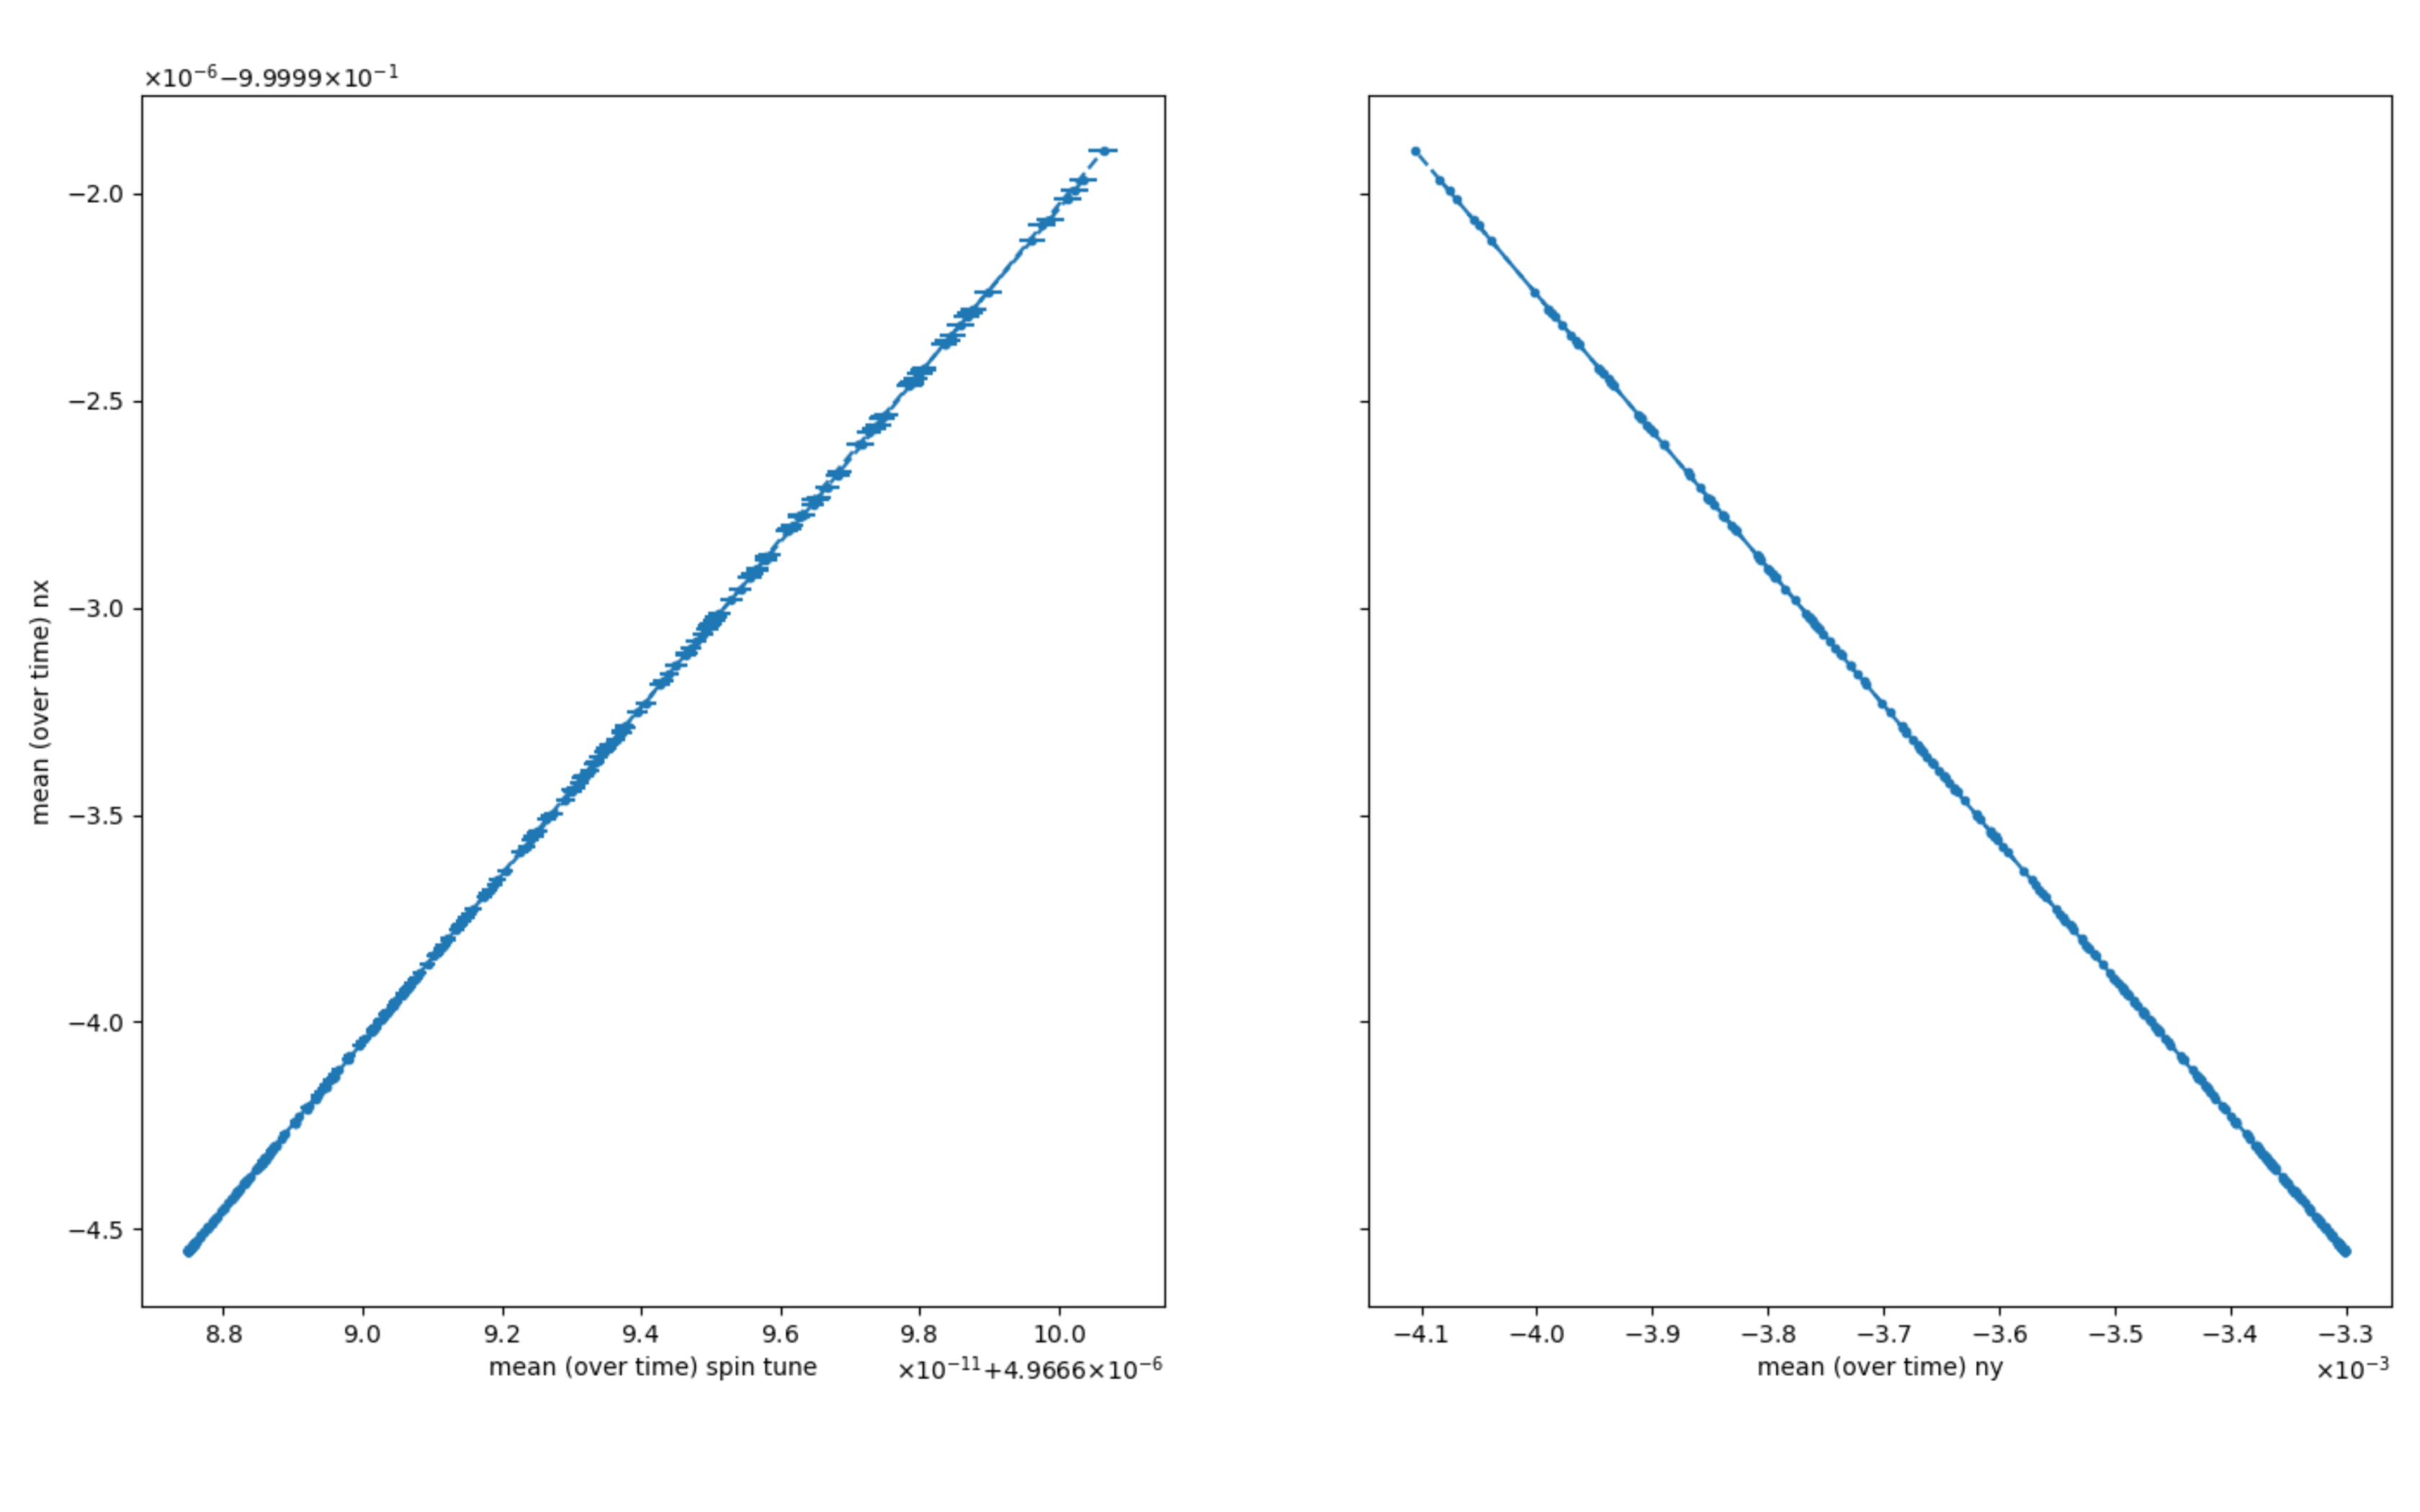
\includegraphics[width=\linewidth]{images/decoh_sim/mean_n_bar_vs_spin_tune}
	\caption{Средние уровни поперечных компонент осей стабильного спина частиц, в зависимости от уровня их спин-тюна.\label{decoh:fig:nbar_vs_ST}}
\end{figure}

\subsection{Анализ механизма подавления декогеренции секступольными полями}\label{sec:sext_decoh_suppression_effect_analysis}
Исходя из уравнений~\eqref{eq:spin_tune_vs_gamma} и~\eqref{eq:EquLevMom_shift}, зависмость спин-тюна от равновесной энергии частицы можно выразить следующим образом:
\[
\nu_s = G\gamma_0 + G\frac{\gamma_0^2-1}{\gamma_0}\cdot C_0\cdot f_1(\epsilon_x, \epsilon_y, Q_x, Q_y)+ G\frac{\gamma_0^2-1}{\gamma_0}\cdot C_0\cdot f_2(\alpha_1, \avg{\Delta K/K}^2),
\]
где $C_0$ константа, а $f_1$ и $f_2$ определяются уравнением~\eqref{eq:EquLevMom_shift}.

Поскольку частица, совершающая бетатронные колебания, автоматически совершает и синхротронные колебания, эффект секступольных полей на её спин-тюн --- это суперпозиция эффектов. Однако же частица, находящаяся на референсной орбите, но имеющая начальное отклонение по импульсу, имеет такую же длину орбиты, и совершает только синхротронные колебания. Соответственно, секступольные поля влияют на спин-тюн такой частицы только путём модификации коэффициента сжатия орбиты, т.е. функции $f_2$. 

В связи с этим, мы провели симуляцию, в которой последовательно инжектировали два пучка по 30 частиц: в первом, D-банче, частицы были распределены как $\delta\sim N(0, 0.5\cdot 10^{-6})$, во втором, Y-банче, --- $y\sim N(0, 0.5)$ мм. Остальные координаты фазового пространства имели начальное значение равное нулю. 

Пучки инжектировались в идеальную структуру, для того, чтобы исключить эффекты, связанные с возмущением орбит нереференсных частиц. Для первого пучка были включены только GSD секспутоли, для второго --- GSY. Градиенты секступолей варьировались $\pm 5\cdot 10^{-3}$ от оптимального значения соответствующего семейства.

Трекинг проводился на протяжении $1.2\cdot 10^6$ оборотов, данные выводились каждые 800 оборотов.

На Рисунке~\ref{fig:long_PS_sext_settings} представлены фазовые траектории частиц пучков в продольном фазовом пространстве. Мы видим, что фазовые эллипсы частиц D-банча центрированы практически~\footnote{При увеличении можно наблюдать различие центров фазовых эллипсов, но это различие не чувствительно к значению градиента секступоля, и скорее всего следствие конечности статистики.} на одной и той же точке, а их эмиттансы не меняются при изменении силы поля сексуполя. 

В то же время фазовые портреты частиц Y-банча меняются при изменении значения градиента секступоля. При этом мы видим, что максимальная скученность их центров (следовательно равновесных уровней энергии) не соответствует оптимальному значению градиента секступоля (фазовый портрет для последнего изображён на центральной панели). Именно это наблюдение послужило для нас стимулом инжекции в структуру D-банча. Мы объясняем это наблюдение суперпозицией эффектов сжатия равновесных орбит частиц, и модификации коэффициента сжатия орбиты.

\begin{figure}[h]
	\centering
	\subbottom[Фазовые эллипсы D-банча.]{%
		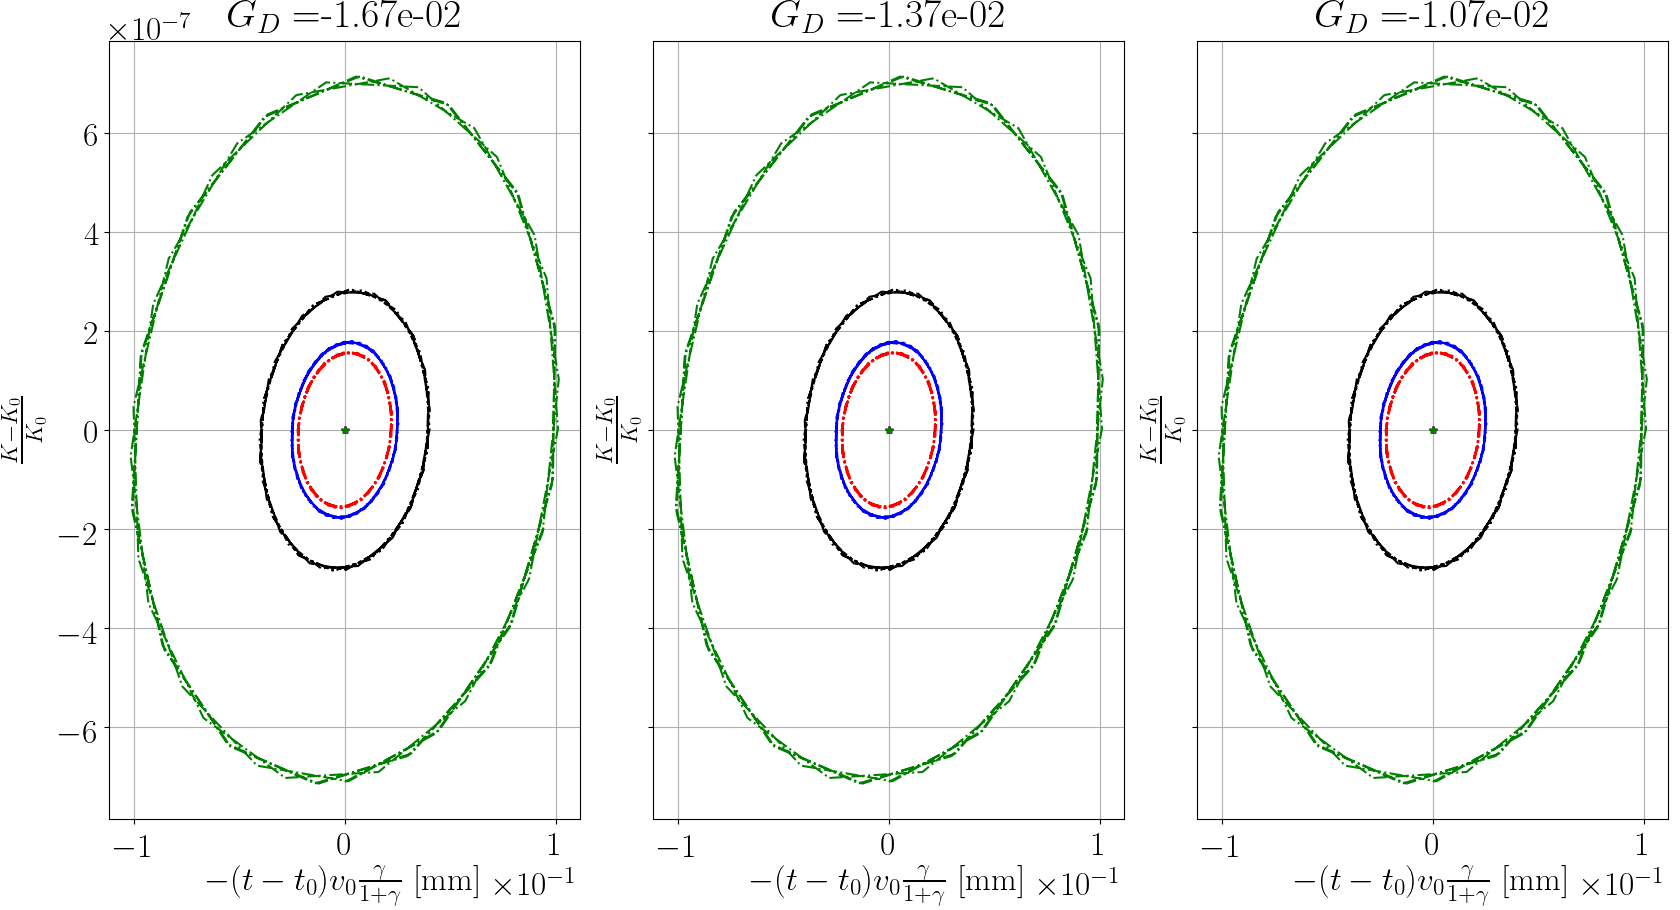
\includegraphics[width=\linewidth]{images/decoh_sim/propdef/long_phase_space_for_sext_settings_D}
	}
	\subbottom[Фазовые эллипсы Y-банча.]{%
		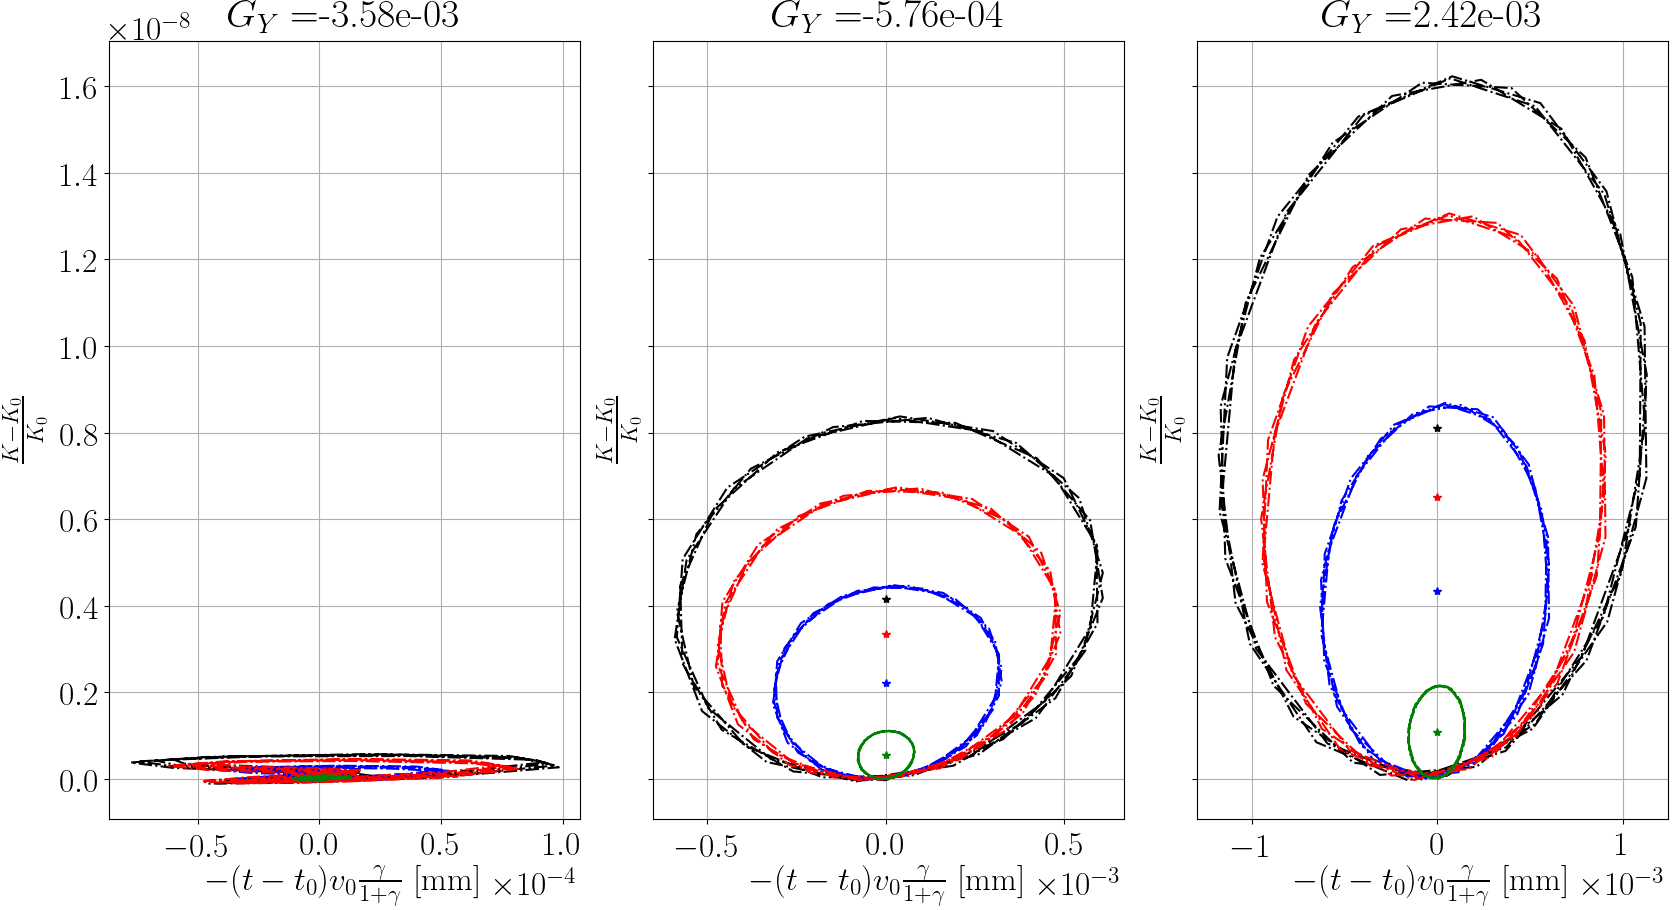
\includegraphics[width=\linewidth]{images/decoh_sim/propdef/long_phase_space_for_sext_settings_Y}
	}
	\legend{Цветом различаются траектрории частиц с разным начальным вертикальным смещением от замкнутой орбиты.}
	\caption[Продольное фазовое пространство пучка. Звёздочками отмечены центры эллипсов]{Продольное фазовое пространство пучка. Звёздочками отмечены центры эллипсов.\label{fig:long_PS_sext_settings}}
\end{figure}

Для более тщательного рассмотрения эффектов секступоля на функции $f_1$ и $f_2$, мы построили зависимости средних уровней спин-тюнов частиц от их равновесных уровней энергии (Рисунок~\ref{fig:ST_vs_dkok_for_sext_strenghts}). Мы видим, что скученность точек графика для D-банча не меняется при варьировании значения градиента секступоля, а меняется только функциональная зависимость спин-тюна от равновесной энергии, как и предполагается функциональной формой $f_2$ (см. раздел~\ref{chpt1:FS-methods:effective-Lorentz-factor}). Таким образом, сигнатурой оптимизации коэффициента сжатия орбиты служит изменение функциональной зависимости $\avg{\nu_s} = f(\avg{\Delta K/K})$.

На рисунке для Y-банча наблюдаются оба эффекта секступольного подавления декогеренции: изменяется и скученность точек (т.е. эмиттанс пучка), и функциональная зависимость.

\begin{figure}[h]
	\centering
	\subbottom[Для D-банча.]{%
		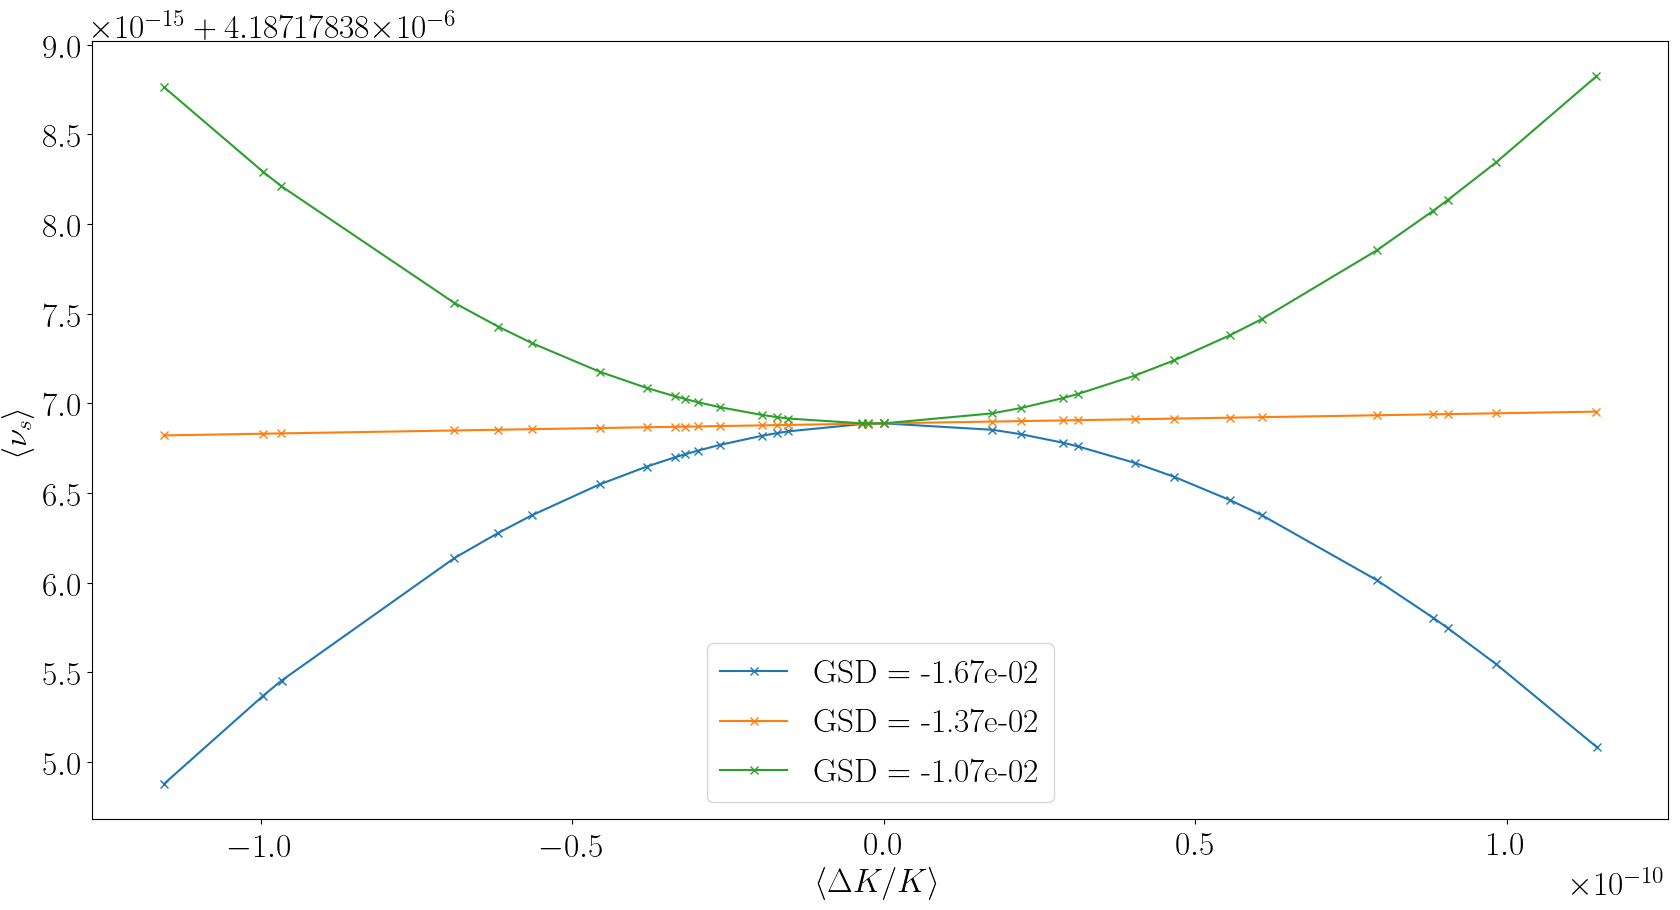
\includegraphics[width=\linewidth]{images/decoh_sim/propdef/stune_vs_dkok_SS_D}
	}
	\subbottom[Для Y-банча.]{%
		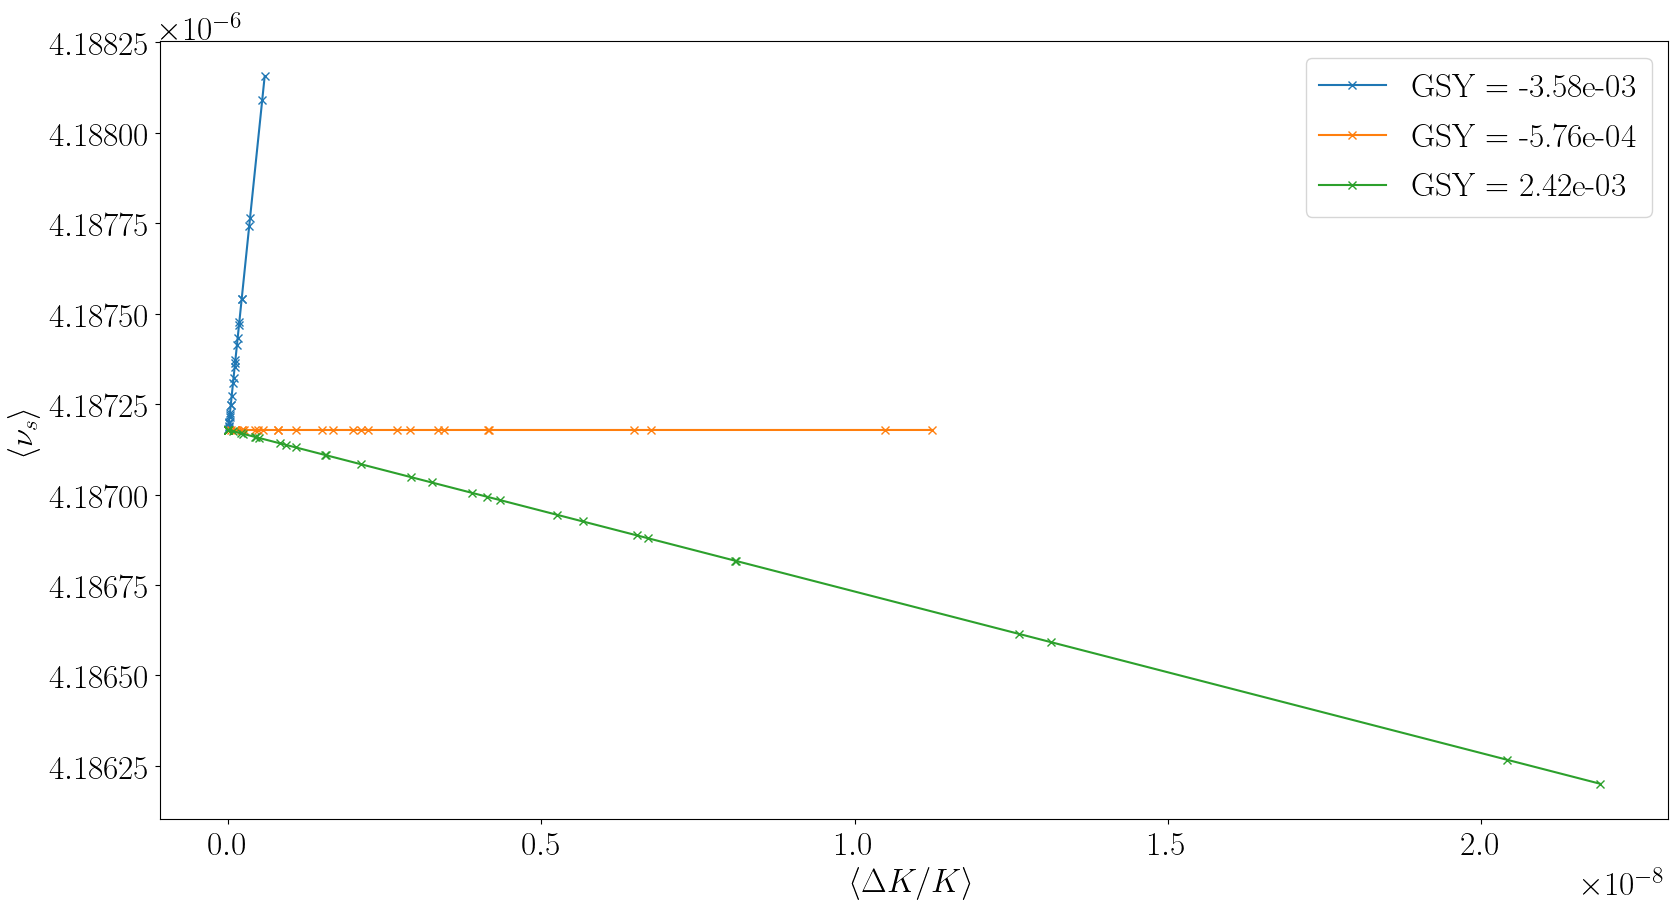
\includegraphics[width=\linewidth]{images/decoh_sim/propdef/stune_vs_dkok_SS_Y}
	}
	\caption{Зависимость среднего уровня спин-тюна частицы от её равновесного уровня энергии для различных значений градиента секступоля.\label{fig:ST_vs_dkok_for_sext_strenghts}}
\end{figure}

\paragraph{Вывод:} Симуляция подтверждает утверждения~\eqref{eq:Sext_compaction_effect} и~\eqref{eq:Sext_OL_effect}.

\section{Ошибки неидеальности ускорителя}\label{chpt3:imperfections}
Систематические ошибки, вызванные физическими неидеальностями
ускорителя, включая неточность юстировки оптических элементов,
вызывают фальш-сигнал ЭДМ.~\cite[стр.~230]{Eremey:Thesis} Особенно в
этом отношении проблематичны наклоны элементов вокруг оптической оси, поскльку они
индуцируют паразитную горизонтальную компоненты магнитного поля $B_x$, 
вращающую спин-вектор частицы в вертикальной плоскости; той, в которой измеряется ЭДМ.

Аналитические оценки МДМ частоты прецессии спина вокруг радиальной оси 
были сделаны в~\cite{Senichev:FDM}. 
Из уравнения Т-БМТ, и выражения силы Лоренца,
скорость МДМ прецессии вокруг радиальной оси выражается как
\begin{equation}\label{eq:tilted-MDM-precession-freq}
\SD{\W_x^{MDM}} = \frac{q}{m\gamma}\frac{G+1}{\gamma}\frac{\SD{B_x}}{\sqrt{n}},
\end{equation}
где $n$ число наклонённых спин-ротаторов, и ${\SD{B_x} = B_y\SD{\delta h}/L}$, 
при стандартном отклонении ошибки юстировки
$\SD{\delta h}$. При величине ошибки ${\SD{\delta h} = 100}$~мкм, и
длине дефлектора $L=1$~м, ${\SD{\W_x^{MDM}} \approx 100}$~рад/сек.~\cite{Senichev:FDM}

Мы изучили спиновую динамику в структуре с замороженным спином 
в присутствии наклонов оптических элементов с помощью кода COSY INFINITY. 
Результаты нашей симуляции согласуются с оценками, представленными выше.


\paragraph{Имплементация паразитного поля}\label{chpt3:imperfections:implementation}
Имплементируя неидеальности полей, мы следовали рекомендациям
изложенным в~\cite[стр.~235]{Eremey:Thesis}. Малое возмущение
магнитного поля, в первом приближении, действует как маленький пропорциональный поворот
спин-вектора (спин-кик). Поэтому мы имплементировали наклон E+B элемента как
домножение соответствующей матрицы поворота на его спиновую трансфер-матрицу.
Такая имплементация наклона элемента гарантирует сохранение 
замкнутой орбиты; физически, сохранение замкнутой орбиты обусловлено 
появлением компенсирующего электрического поля спин-ротатора при его наклоне.

В соответствии с уравнением~\eqref{eq:TBMT_MDM}, изменение МДМ частоты
прецессии, ассоциированное с введённым паразитным полем $(B_x, 0, B_z)$ есть
\begin{align*}
	\Delta\W_{MDM} &= \frac qm G \cdot (B_x, 0, B_z),
	\intertext{поэтому угол спин-кика равен}
	\Theta_{kick} &= t_0\Delta\W_{MDM},
\end{align*}
где $t_0 = L/v_0$ пролётное время референсной частицы через элемент.

\subsection{Зависимость от распределения неидеальностей} \label{chpt3:imperfections:magnitude}
Данная серия симуляций была проведена с целью подтвердить два тезиса
касательно систематической ошибки измерения частоты прецессии спина вокруг
радиальной оси, вызванной неточностью установки E+B элементов:
\begin{enumerate*}[(1)]
	\item индуцированный МДМ-эффект зависит только от среднего значения
	угла наклона элементов, но не от  конкретной последовательности
	углов; и
	\item эта зависимость носит линейный характер.
\end{enumerate*}

Симуляция была проведена следующим образом: мы распределили наклоны
$\Theta_{tilt}$ E+B элементам FS структуры случайным образом. После
построения трансфер-матриц (спиновой и орбитальной) до  3-го порядка разложения Тэйлора, 
были вычислены разложения Тэйлора функций спин-тюна и оси прецессии спина (SPA). Члены нулевого
порядка последних представляют собой спин-тюн и SPA референсной частицы.

Угловая скорость поворота спин-вектора референсной частицы вычисляется по формуле:~\cite[стр.~4]{COSY:SpinTuneMapping}
\[
\vec\W = 2\pi/\tau_0\cdot \nu_s \cdot \bar n,
\]
где $\tau_0 = f^{-1}_{rev} = 10^{-6}$ секунд есть пролётное время частицы через ускоритель.

Симуляция была проведена 11 раз. Каждый раз углы наклона
спин-ротаторов выбирались из нормального распределения
$N(\mu_0\cdot(i-5), \sigma_0)$, где ${\mu_0 = 10\cdot \sigma_0 =10^{-4}}$~рад, 
${i\in\lbrace0,\dots, 10\rbrace}$. Результаты представлены
на Рисунке~\ref{fig:Linearity_test_shifting_gauss}.

\begin{figure}[H]
	\centering
	\subbottom[Компоненты оси прецессии $\nbar$]{%
		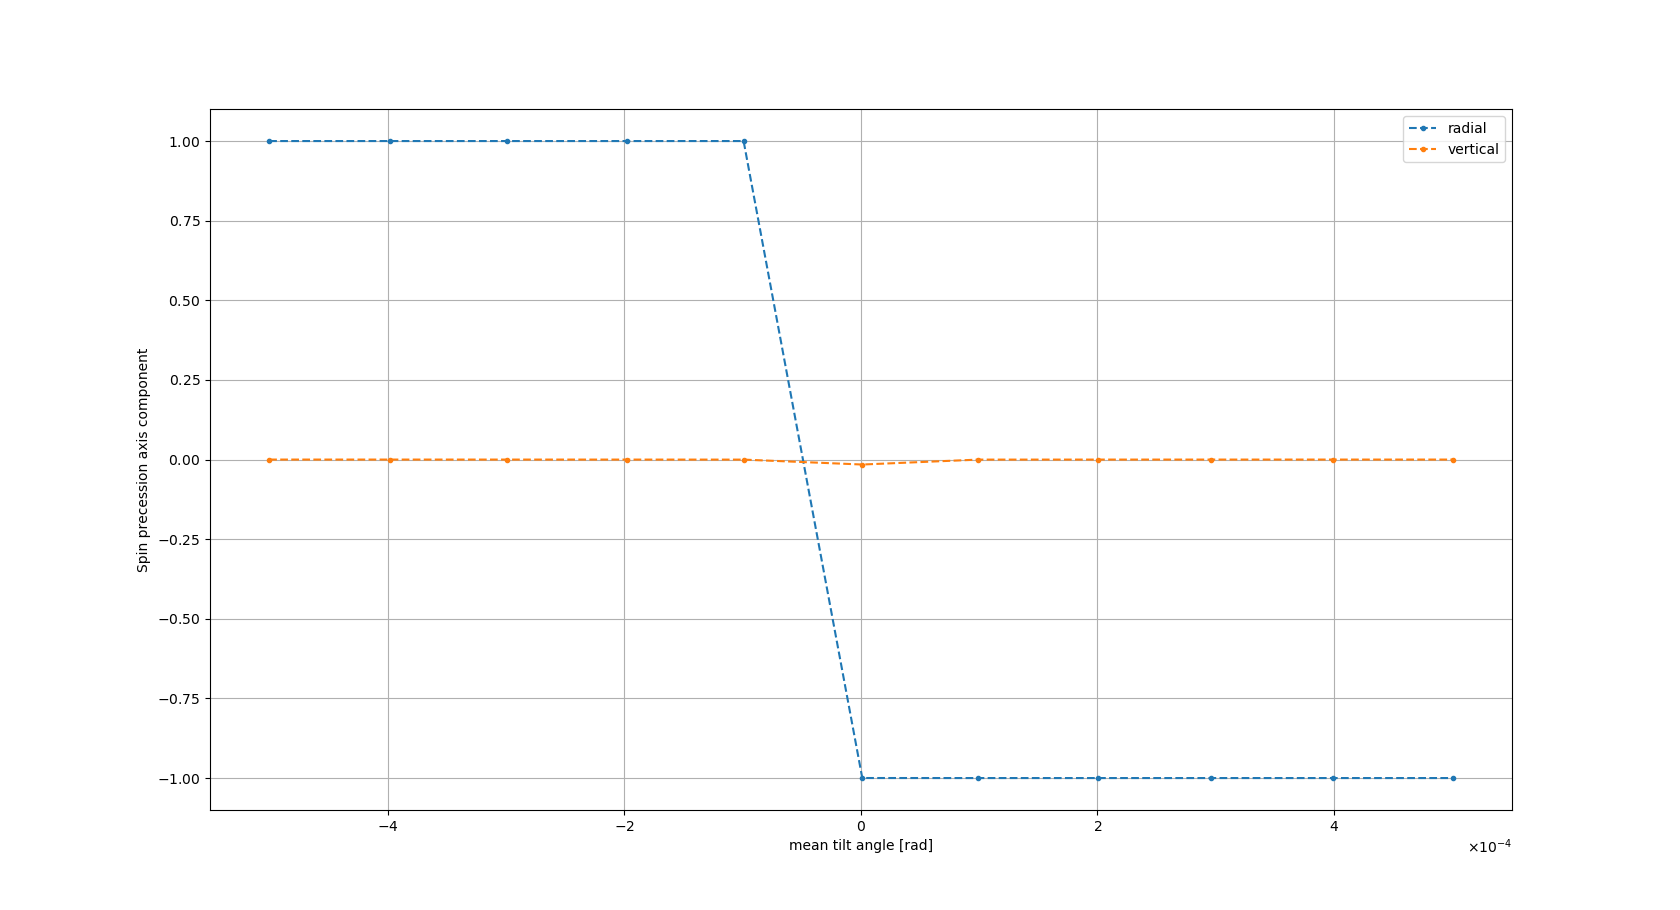
\includegraphics[height=.35\paperheight]{images/fake_signal_sim/linearity_test_shifting_gauss_nbar}}
\end{figure}
\begin{figure}[H]\centering
	\contsubbottom[Компоненты частоты прецессии $\vec\W$]{%
		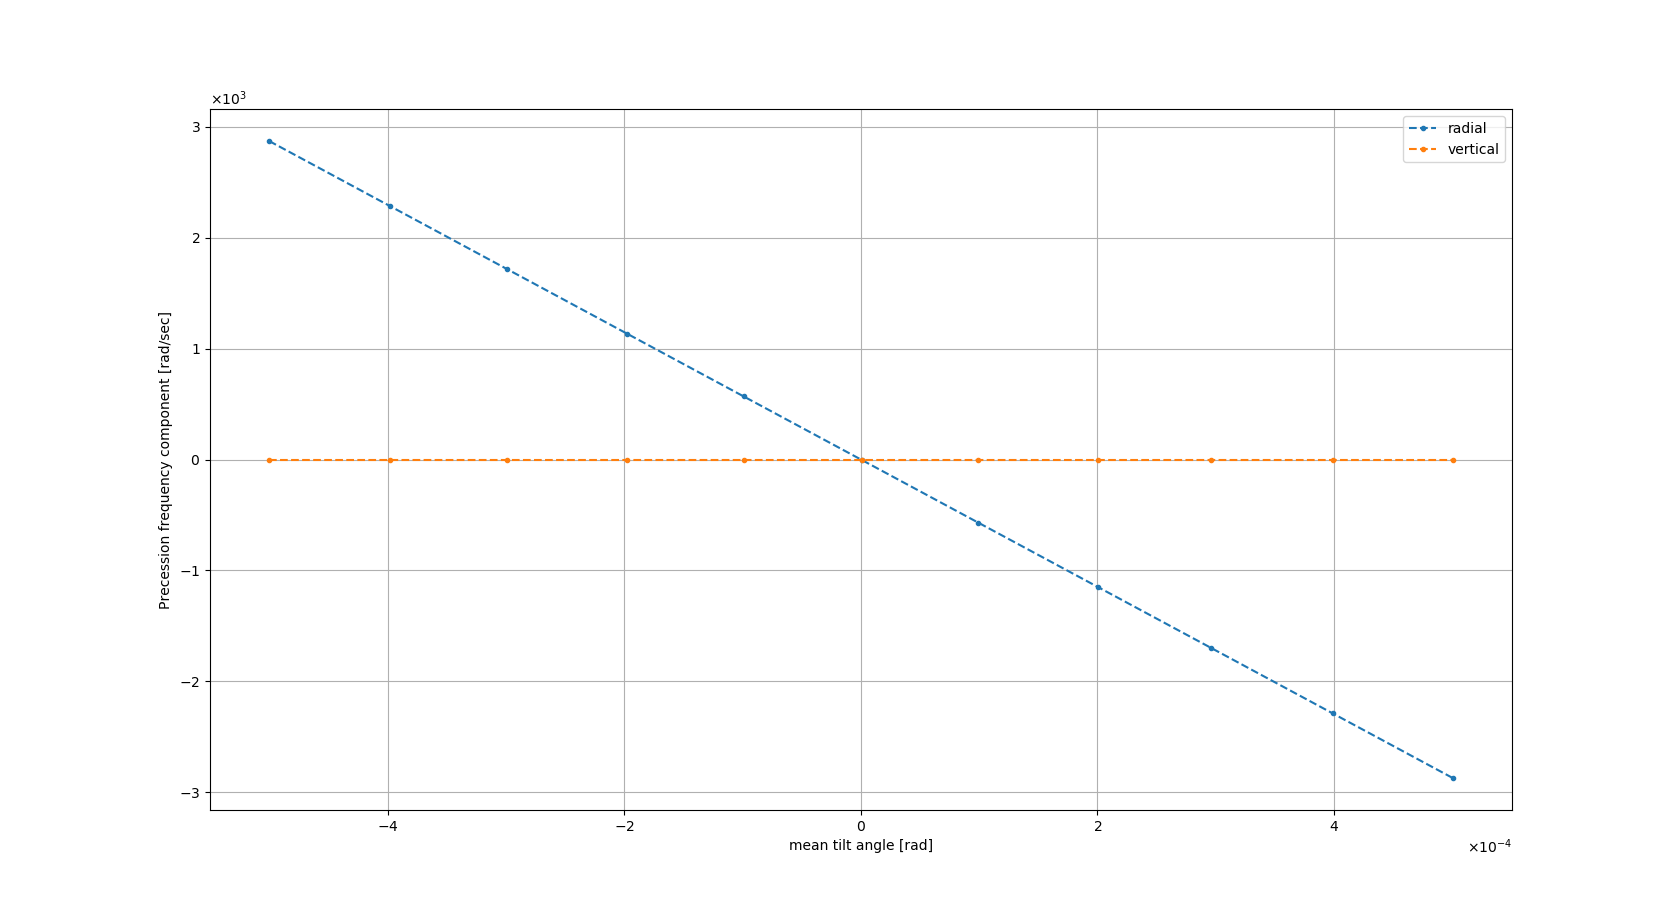
\includegraphics[height=.35\paperheight]{images/fake_signal_sim/linearity_test_shifting_gauss_freq}}
	\legend{Цветом различаются радиальная (синий) и вертикальная (оранжевый) компоненты векторов $\bar n$, $\vec\W$.}
	\caption{Зависимость направления и частоты прецессии спина референсной частицы в неидеальной FS-структуре со случайно-распределёнными ошибками установки спин-ротаторов от их среднего угла наклона.\label{fig:Linearity_test_shifting_gauss}}
\end{figure}

Из рисунка видно, что при такой установке элементов, при которой среднее значение угла наклона равно 
$10^{-4}$~рад, поляризация пучка будет вращаться в вертикальной плоскости с угловой срокостью 
около 500~рад/сек. Это согласуется с оценками выше (раздел~\ref{chpt3:imperfections},
 ур-е~\eqref{eq:tilted-MDM-precession-freq}), поскольку в них предполагается 
 стандартное отклонение ошибки наклона $10^{-4}$~рад, а также наклон ${n=100}$ элементов. 
 В этом случае, стандартное отклонение среднего угла наклона элементов равно $10^{-5}$~рад, и значит, 
 с вероятностью 67\%, МДМ спин-прецессия вокруг радиальной оси будет происходить со скоростью 
 до 50~рад/сек, а с вероятностью 95\% --- до 100~рад/сек.

На Рисунке~\ref{fig:Linearity_test_compensated} изображены результаты теста, в котором 
E+B элементы попарно повёрнуты на противоположные углы (три случайные пары), а один элемент 
повёрнут на угол ${\mu_i = (i-5)\cdot 10^{-6}}$ рад, ${i\in\lbrace0,\dots,10\rbrace}$. Обе симуляции были 
выполнены на энергии 270.0092~МэВ.\footnote{На этой энергии, в идеальной структуре, 
	$\nu_s$ и $\nbar$ не определены в системе координат связанной с пучком, используемой в
	COSY INFINITY. Это соответствует ситуации, когда спин не прецессирует ни в какой плоскости 
	(горизонтальной или вертикальной), что есть условие трёхмерно-замороженного спина, 
	для идеальной структуры.} Можно наблюдать, что скомпенсированные элементы не дают вклад во вращение
спин-вектора референсной частицы.

\begin{figure}[H]
	\centering
	\subbottom[Компоненты оси прецессии $\nbar$]{%
		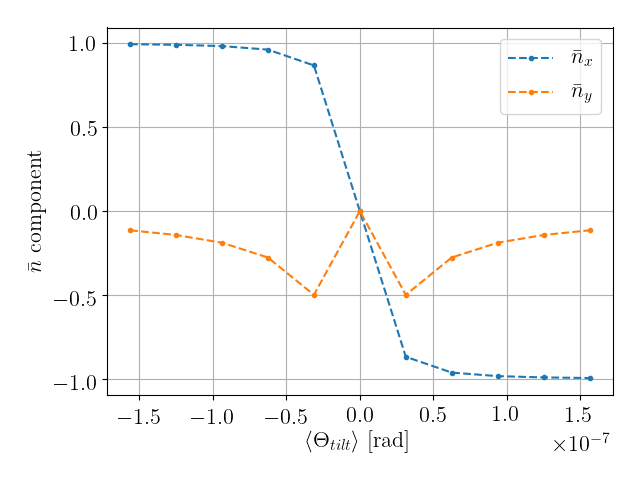
\includegraphics[height=.35\paperheight]{images/fake_signal_sim/linearity_test_compensated+microrad_nbar}}
\end{figure}
\begin{figure}[H]\centering
	\contsubbottom[Компоненты частоты прецессии $\vec\W$]{%
		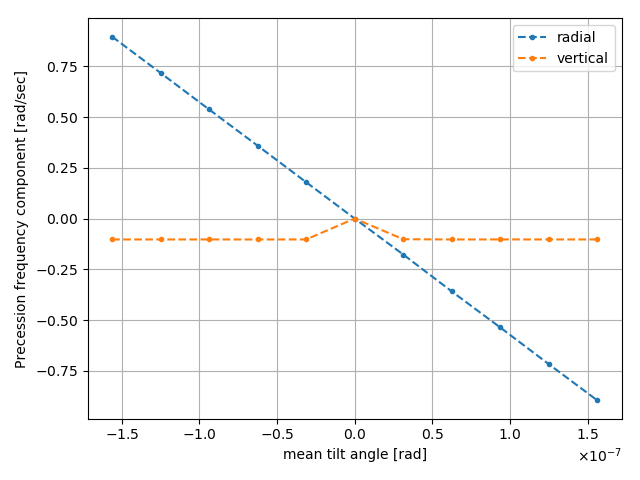
\includegraphics[height=.35\paperheight]{images/fake_signal_sim/linearity_test_compensated+microrad_freq}}
	\caption{Зависимость направления и частоты прецессии спина референсной частицы в неидеальной FS-структуре в случае попарно-компенсированных ошибок установки спин-ротаторов от их среднего угла наклона.\label{fig:Linearity_test_compensated}}
\end{figure}



\subsection{Равенство частот прецессии спинов частиц при движении в прямом и обратном направлениях}\label{chpt3:imperfections:CW_vs_CCW}
На Рисунке~\ref{fig:Lin_test_rel_diff} изображена относительная разница между значениями
радиальной компоненты оси стабильного спина $\nbar_x$ (частоты спин-прецессии $\W_x$) частицы, 
при движении пучка по часовой (CW) или против часовой (CCW) стрелки, соответственно для случаев 
случайно-распределённой ошибки наклона элементов, и при попарной компенсации наклонов.

Для радиальной компоненты оси стабильного спина, относительная разница вычислялась как 
\[
\delta\nbar_x = \frac{\nbar_x^{CW}(\avg{\Theta_{tilt}}) - \nbar_x^{CCW}(\avg{\Theta_{tilt}})}{\nbar_x^{CW}(\avg{\Theta_{tilt}})};
\]
для частоты, соответственно:
\[
\delta\W_x = \frac{\W_x^{CW}(\avg{\Theta_{tilt}}) - \W_x^{CCW}(\avg{\Theta_{tilt}})}{\W_x^{CW}(\avg{\Theta_{tilt}})}.
\]

Из рисунков следует, что при движении пучка в любом из направлений, ось стабильного спина 
наклонена одинаково; при этом существует \emph{различие} между спин-тюнами CW и CCW пучков, но 
на уровне не более десятых долей процента, которое тем сильнее, чем меньше модуль частоты спин-прецессии. 
Эта \emph{разница}  свидетельствует об асимметричности ускорительной структуры 
относительно обращения направления движения, с точки зрения спиновой динамики, 
и может объясняться различием референсных орбит прямого и обратного пучков. 

\begin{figure}[H]
	\centering
	\subbottom[Случайно-распределённые наклоны E+B элементов]{%
		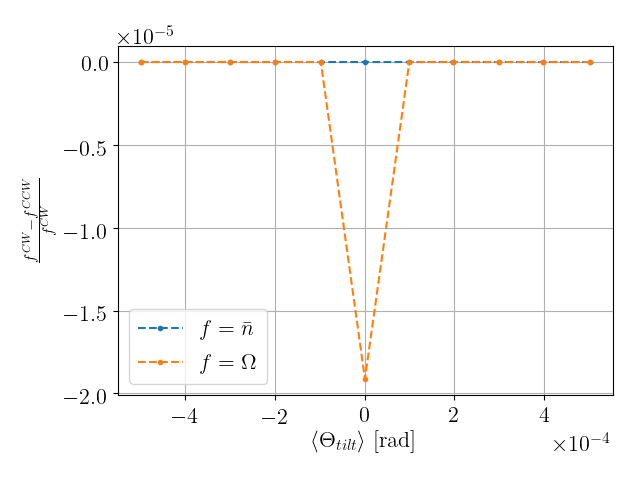
\includegraphics[height=.35\paperheight]{images/fake_signal_sim/linearity_test_shifting_gauss_rel_diff}	
	}
\end{figure}
\begin{figure}[H]\centering
	\contsubbottom[Попарно-компенсированные наклоны]{%
		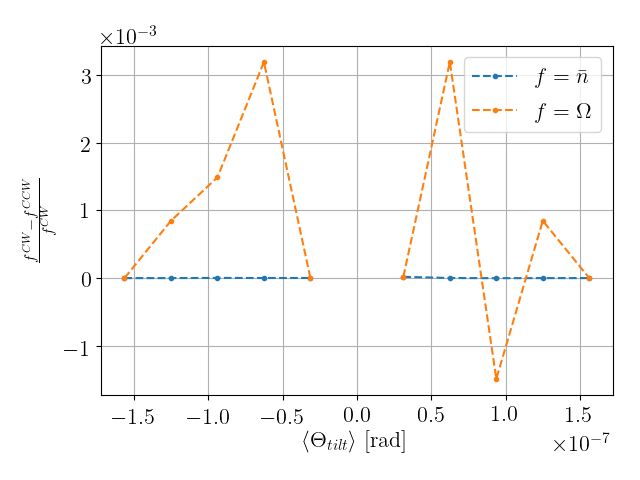
\includegraphics[height=.35\paperheight]{images/fake_signal_sim/linearity_test_compensated+microrad_rel_diff}
	}
	\legend{Цветом обозначена разница между радиальными компонентами (синий) оси стабильного спина, (оранжевый) частоты спин-прецессии CW и CCW пучков}
	\caption{Относительная разница между радиальными компонентами оси стабильного спина и угловой скоростью поворота спина, посчитанная относительно значения для CW-циркулирующего пучка\label{fig:Lin_test_rel_diff}}
\end{figure}


\section{Смена полярности ведущего поля}\label{chpt3:GFF}
Необходимо уделить внимание двум аспектам проблемы смены полярности ведущего поля:
\begin{enumerate}
	\item Какой параметр системы должен оставаться постоянным от цикла к циклу;
	\item Как его можно наблюдать.
\end{enumerate}

Целью смены полярности ведущего поля является точное воспроизведение радиальной компоненты
частоты МДМ прецессии $\errmdm$, индуцированной полями неидеальности оптической структуры ускорителя. 
Этот момент часто упускается из виду: простое воспроизведение величины \textbf{магнитного поля} не достаточно,
 поскольку точка инжекции центра масс пучка, а значит его длина орбиты --- и соответственно, 
 ввиду уравнений~\eqref{eq:EffectiveGamma} и~\eqref{eq:spin_tune_vs_gamma}, спин-тюн --- 
 подвержена вариации.~\footnote{Помимо этого, 
 	ускорительная структура может быть асимметрична, с точки зрения спиновой динамики, 
 	относительно обращения направления движения пучка.}

Таким образом, необходимо восстанавливать не величину поля, а эффективный Лоренц-фактор центра масс пучка.

Для калибровки эффективного Лоренц-фактора, в FD-методе измеряется вертикальная компонента
ЭДМ+МДМ частоты спин-прецессии $\W_y$; пучок при этом выводится из состояния ``замороженного спина.'' 
В этой ситуации, 
\begin{align*}
	\vec\W_{EDM} &= \ux\cdot \W_{EDM} + \uy\cdot \erredm, \\
	\vec\W_{MDM} &= \ux\cdot \errmdm + \uy\cdot \W_{MDM}, 
	\intertext{где связанные с полями неидеальности оптической структуры частоты}
	\erredm  &= f_{EDM}(E_y, B_x)   \ll \W_{EDM}, \\
	\errmdm &= f_{MDM}(E_y, B_x)  \ll \W_{MDM}.
	 \intertext{Тогда}
	\vec\W  &= \vec\W_{EDM} + \vec\W_{MDM} \\
				&= \ux\cdot (\errmdm+ \W_{EDM}) + \uy\cdot  (\erredm+\W_{MDM}).
	\intertext{Ввиду того, что измеряемый ЭДМ-эффект $\W_{EDM}$ значительно превосходит $\erredm$:}
	\erredm &\ll \W_{EDM} \ll \errmdm \ll \W_{MDM},
\end{align*}
в первом приближении, когда мы манипулируем вертикальной компонентой 
${\W_y = \erredm + \W_{MDM}}\approx \W_{MDM}$, 
мы манипулируем вертикальной компонентой вектора угловой скорости МДМ-прецессии $\W_{MDM}$.
Последняя же однозначно связана с $\errmdm$.


\newcommand{\Traj}{\mathcal T}
\DeclareDocumentCommand{\Stab}{s}{\mathcal{S}\IfBooleanT{#1}{\vert_{\W_y=0}}}
\newcommand{\Fail}{\mathcal F}
\DeclareDocumentCommand{\g}{s}{\gamma\IfBooleanT{#1}{_{eff}}}
\newcommand{\CO}{\mathrm{CO}}


\subsection{Алгоритм калибровки}
Пусть $\Traj$ обозначает множество всех возможных траекторий частицы в ускорителе. $\Traj = \Stab \bigcup \Fail$,
где $\Stab$ это все стабильные траектории, а $\Fail$ --- это такие траектории,
при попадании на одну из которых частица теряется из пучка.

Калибровка производится в два этапа:
\begin{enumerate}
\item На первом этапе величина поля выставляется таким образом, чтобы частицы инжектированного пучка
попадали на траектории $t\in \Stab$. В первом приближении, это будет та же величина,
что и для обратно-йиркулирующего пучка, но с противоположным знаком.
\item Затем величина поля уточняется, путём удовлетворения условия замороженности спина в горизонтальной
плоскости. При выполнении этого условия, из $\Stab$ выбирается подмножество $\Stab*$ тракеторий, для которых
$\W_y = 0$.
\end{enumerate}

Предположим, что $\W_y = \W_y(\g*)$ --- инъективная функция, а значит
$\W_y(\g*^1) = \W_y(\g*^2) \rightarrow \g*^1 = \g*^2$. Пространство траекторий делится на
классы эквивалентности по величине эффективного Лоренц-фактора: траектории с одинаковым $\g*$ эквивалентны
с точки зрения спин-динамики (то есть, обладают одним и тем же значением спин-тюна $\nu_s$ и направлением
оси стабильного спина $\nbar$), и принадлежат одному классу. Поскольку $\W_y$ инъективная, значит существует
уникальное $\g*$, один класс эквивалентности, при котором $\W_y=0$: $[\W_y=0]\equiv [\g*^0] = \Stab*$.

Если бы в структуре кольца не использовались секступоли, $\Stab*$ было бы синглетоном (множеством с
единственным элементом). В разделе~\ref{chpt3:decoherence}, мы уже показали, что
при использовании секступолей, $\forall t_1,t_2\in\Stab*$:
$\nu_s(t_1) = \nu_s(t_2)$, $\nbar(t_1) = \nbar(t_2)$, и значит $\Stab*$ содержит
несколько траекторий.~\footnote{Строго говоря, как видно из симуляций рисунка~\ref{decoh:fig:ST_vs_y0_GSY}
раздела~\ref{chpt3:decoherence}, даже при использовании секступольных полей, сохраняется некоторая,
пренебрежимо малая, зависимость спин-тюна от эффективного Лоренц-фактора. В связи с этим, равенства
здесь приближённые, и множество $\Stab*$ следует считать нечётким множеством: мы будем полагать траектории,
на которых $|\W_y| < \delta$ для некоторого малого $\delta$, как принадлежащими классу $[\W_y=0]$.}

Тогда, чтобы подвтердить валидность калибровочной процедуры, нам нужно показать следующее:
\begin{enumerate}
\item $\Stab*^{CCW} = \Stab*^{CW}$ --- то есть, что и я прямом, и в обратном случае циркуляции пучка,
  $\W_y = 0$ для одних и тех же траекторий (эквивалентно, $\W_y=0$ при одном и том же $\g*$ и в CW, и в CCW
  случаях);
\item $\forall t_1,t_2\in\Stab*^{CCW}$: $\nu_s(t_1) = \nu_s(t_2)$, $\nbar(t_1) = \nbar(t_2)$ ---
  то есть, те же самые секступольные поля подавляют декогеренцию и прямого, и обратного пучков.
\end{enumerate}

Для выполнения этой задачи мы:
\begin{enumerate}
\item строим зависимости $\nu_s(z),~z\in\{x,y,\delta\}$
\end{enumerate}


%% Частоты прецессии спинов частиц пучка определяются по формуле~\cite[стр.~4]{COSY:SpinTuneMapping}
%% \[
%% (\w_x, \w_y, \w_z) = 2\pi\cdot f_{rev} \cdot \nu_s \cdot \bar n,
%% \]
%% где $f_{rev}$ есть циклотронная частота частицы, а $\nu_s$ и $\bar n$ --- её спин-тюн, и ось стабильного спина,
%% соответственно.






\section{Спин-тюн эквивалентность траекторий частиц с одинаковыми значениями эффективного Лоренц-фактора}\label{sec:spin_tune_traj_equivalence}
В контексте процедуры смены направления вращения МДМ спин-прецессии, важно рассмотреть 
вопрос эквивалентности спин-динамики CW и CCW пучков. 

Отправной точкой нашего анализа является утверждение 1: частицы с одинаковым значением эффективного Лоренц-фактора имеют одинаковый спин-тюн, то есть эквивалентны с точки зрения спиновой динамики. Это следствие уравнения~\eqref{eq:spin_tune_vs_gamma}.

В следующих разделах мы проанализируем две формулировки утверждения 1:
\begin{enumerate}[A.]
	\item интерпретируя эффективный Лоренц-фактор как математическое ожидание кинетической энергии частицы;
	\item функция многих переменных $\nu_s(x, a, y, b, \ell, \delta)$ безразлична к фазовой траектории частицы 
	в поперечном фазовом пространстве $(x,a)$, и $(y,b)$, т.е. может быть сведена 
	к функции одной переменной $\nu_s(\g*)$.
\end{enumerate}

\subsection{Формулировка A}

В данном разделе, рассмотрим утверждение 1, интерпретируя эффективный Лоренц-фактор как математическое ожидание Лоренц-фактора частицы.

Для проверки утверждения мы выполнили следующую симуляцию: 
мы инжектировали три банча (X, Y, и D) по 10 частиц в идеальную структуру с замороженным спином. 
Частицы X-банча имели начальное смещение по радиальной координате 
в диапазоне $\pm 1$ мм, Y-банча по вертикальной координате $\pm 1.318$ мм,~\footnote{Такой диапазон 
	принят исходя из требования получить одинаковые эмиттансы частиц, 
	совершающих бетатронные колебания в вертикальной и горизонтальной плоскостях. 
	Начальное отклонение задаёт амплитуду колебаний $A$, 
	которая в свою очередь связана с бета-функцией  $\beta$ и эмиттансом $\epsilon$ частицы 
	как ${A = \sqrt{\epsilon \beta}}$. } а D-банча по энергии,  $\Delta K/K_0$, в диапазоне $\pm 10^{-4}$. 
Орбитальная и спин-трансфер матрицы построены до третьего порядка разложения ряда Тэйлора, 
энергия инжекции 270 МэВ.
Далее проводился трекинг частиц на протяжении 12,000 оборотов, с выводом данных каждые 80 оборотов. 

Данные трекинга: 
\begin{enumerate}[(1)]
	\item координаты частицы в фазовом пространстве ${\vec z = (x,a,y,b,\ell, \delta)}$, 
где ${a=p_x/p_0}$, ${b=p_y/p_0}$ ($p_0$ -- импульс референсной частицы),
${\ell = -(t-t_0)v_0\frac{\gamma_0}{1+\gamma_0}}$ продольное смещение частицы относительно референсной,
${\delta = \Delta K/K}$ --- её смещение по энергии, а также 
\item значение её спин-тюна ${\nu_s(\vec z)}$. 
\end{enumerate}
На основании этих данных, мы вычислили среднее значение спин-тюна $\avg{\nu_s}$, 
среднее значение смещения частицы по энергии $\avg{\Delta K/K}$, продольные и поперечные эмиттансы частиц.

На Рисунке~\ref{fig:stune_traj_equ_main} представлены результаты эксперимента. На верхней панели изображена зависимость $\avg{\nu_s}$ от $\avg{\Delta K/K}$, для бетатрон-осциллирующих банчей, при выключенных секступолях. Из рисунка следует, что при одинаковых средних уровнях энергии, частицы, совершающие бетатронные колебания в вертикальной плоскости, имеют спин-тюн, отличный от частиц, совершающих колебания в горизонтальной плоскости. То есть, на сколько мы можем судить, утверждение 1 в формулировке A опровергнуто.

Мы предположили, что различие наклонов прямых связано с \emph{пространственной зависимостью} коэффициента сжатия орбиты. Это предположение основано на нашем анализе секступольного подавления декогеренции, подробнее описанного в разделе~\ref{sec:sext_decoh_suppression_effect_analysis}. Чтобы проверить наше предположение, мы повторили эксперимент для нескольких значений градиента секступоля GSX, взятых из диапазона $\pm 5\cdot 10^{-3}$.  Результаты представлены на  нижней панели Рисунка~\ref{fig:stune_traj_equ_main}. На рисунке изображена та же зависимость, но только для X-банча, при различных значениях силы поля секступоля. Как видно из рисунка, при варьировании силы поля изменяется наклон касательной зависимости. Точно такое же поведение мы наблюдали и в разделе~\ref{sec:sext_decoh_suppression_effect_analysis}.

\begin{figure}[H]
	\centering
	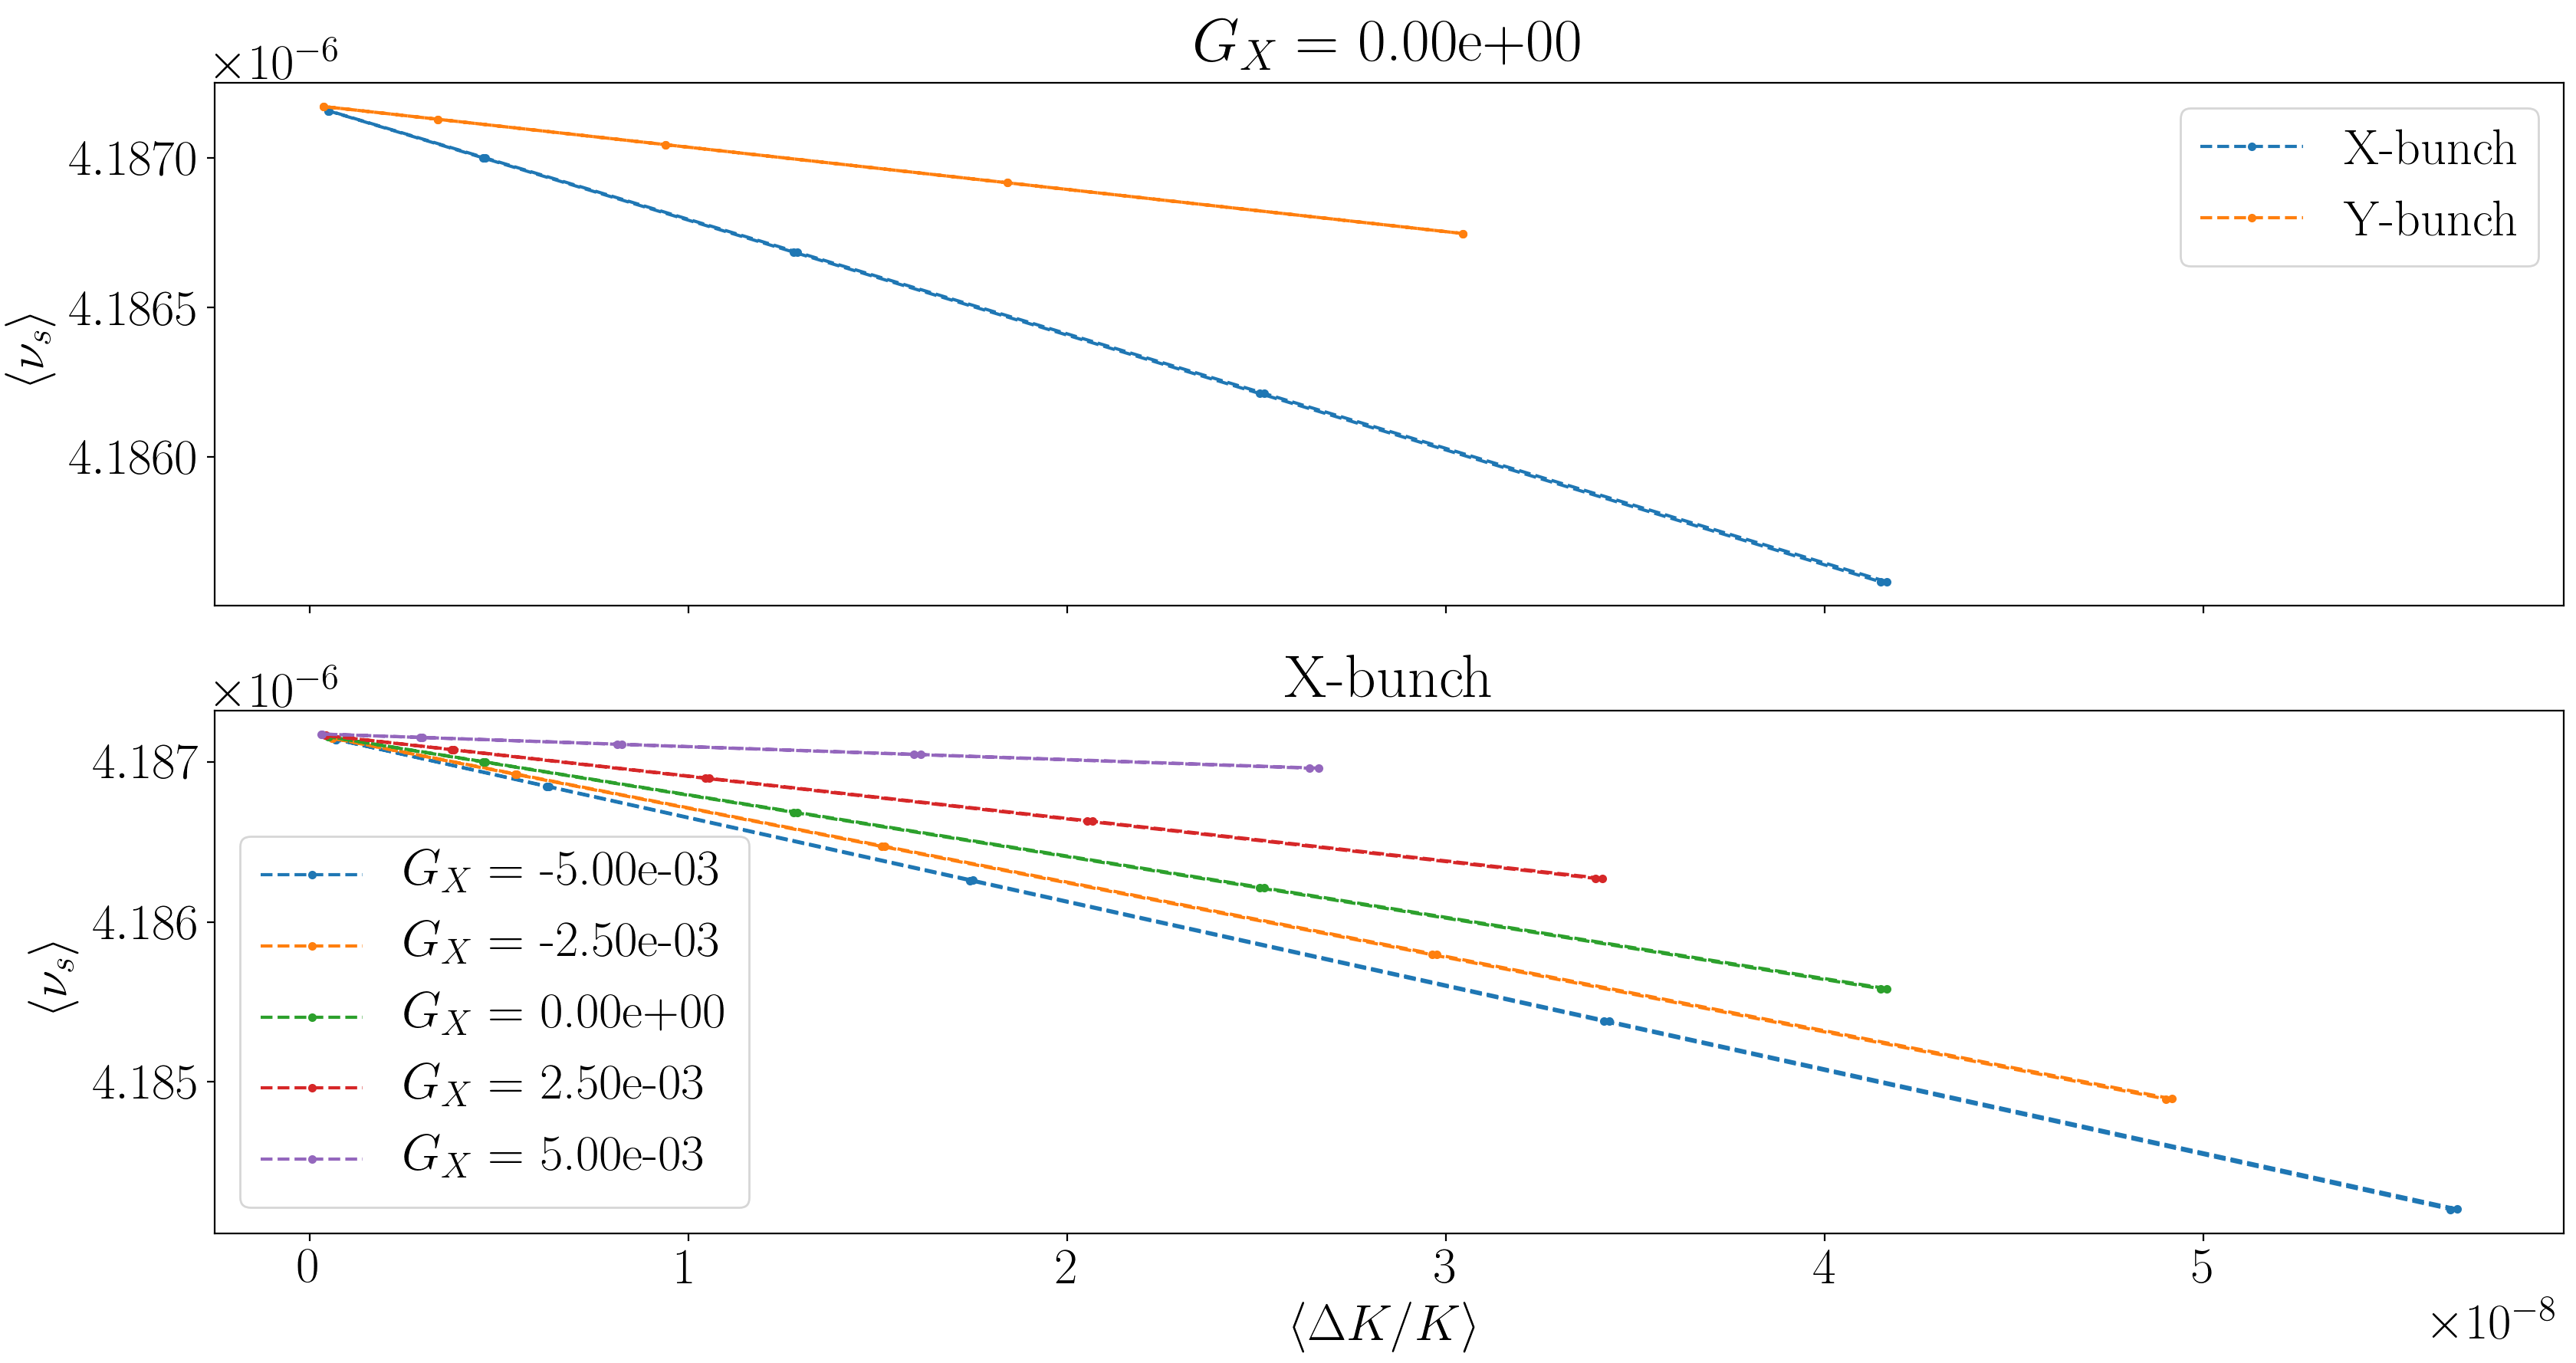
\includegraphics[height=.3\paperheight]{images/stune_traj_equ/part1/stune_vs_equ_energy}
	\caption[Зависимость среднего уровня спин-тюна частицы от её среднего уровня кинетической энергии.]{Зависимость среднего уровня спин-тюна частицы от её среднего уровня кинетической энергии. Верхняя панель: безсекступольный случай, для обоих инжектированных банчей. Нижняя панель: для X-банча, при разных значениях градиента секступоля GSX.\label{fig:stune_traj_equ_main}}
\end{figure}

Для проверки нашей гипотезы о пространственной зависимости коэффициента сжатия орбиты, мы построили зависимости равновесных уровней энергии частиц X-, и Y-банчей от произведения их поперечных эмиттансов и бетатронных тюнов (Рисунок~\ref{fig:equ_nrg_vs_emittance}). Исходя из уравнения~\eqref{eq:betatron_OL}, удлинение орбит с одинаковым произведением поперечного эмиттанса на бетатрон-тюн должно быть одинаковым. Дельта равновесного уровня энергии частицы связана с удлинением её орбиты через коэффициент сжатия орбиты; в связи с этим, разница наклонов прямых на Рисунке~\ref{fig:equ_nrg_vs_emittance} свидетельствует о том, что коэффициенты сжатия орбит разнятся для X-, и Y-банчей. 

\begin{figure}[H]
	\centering
	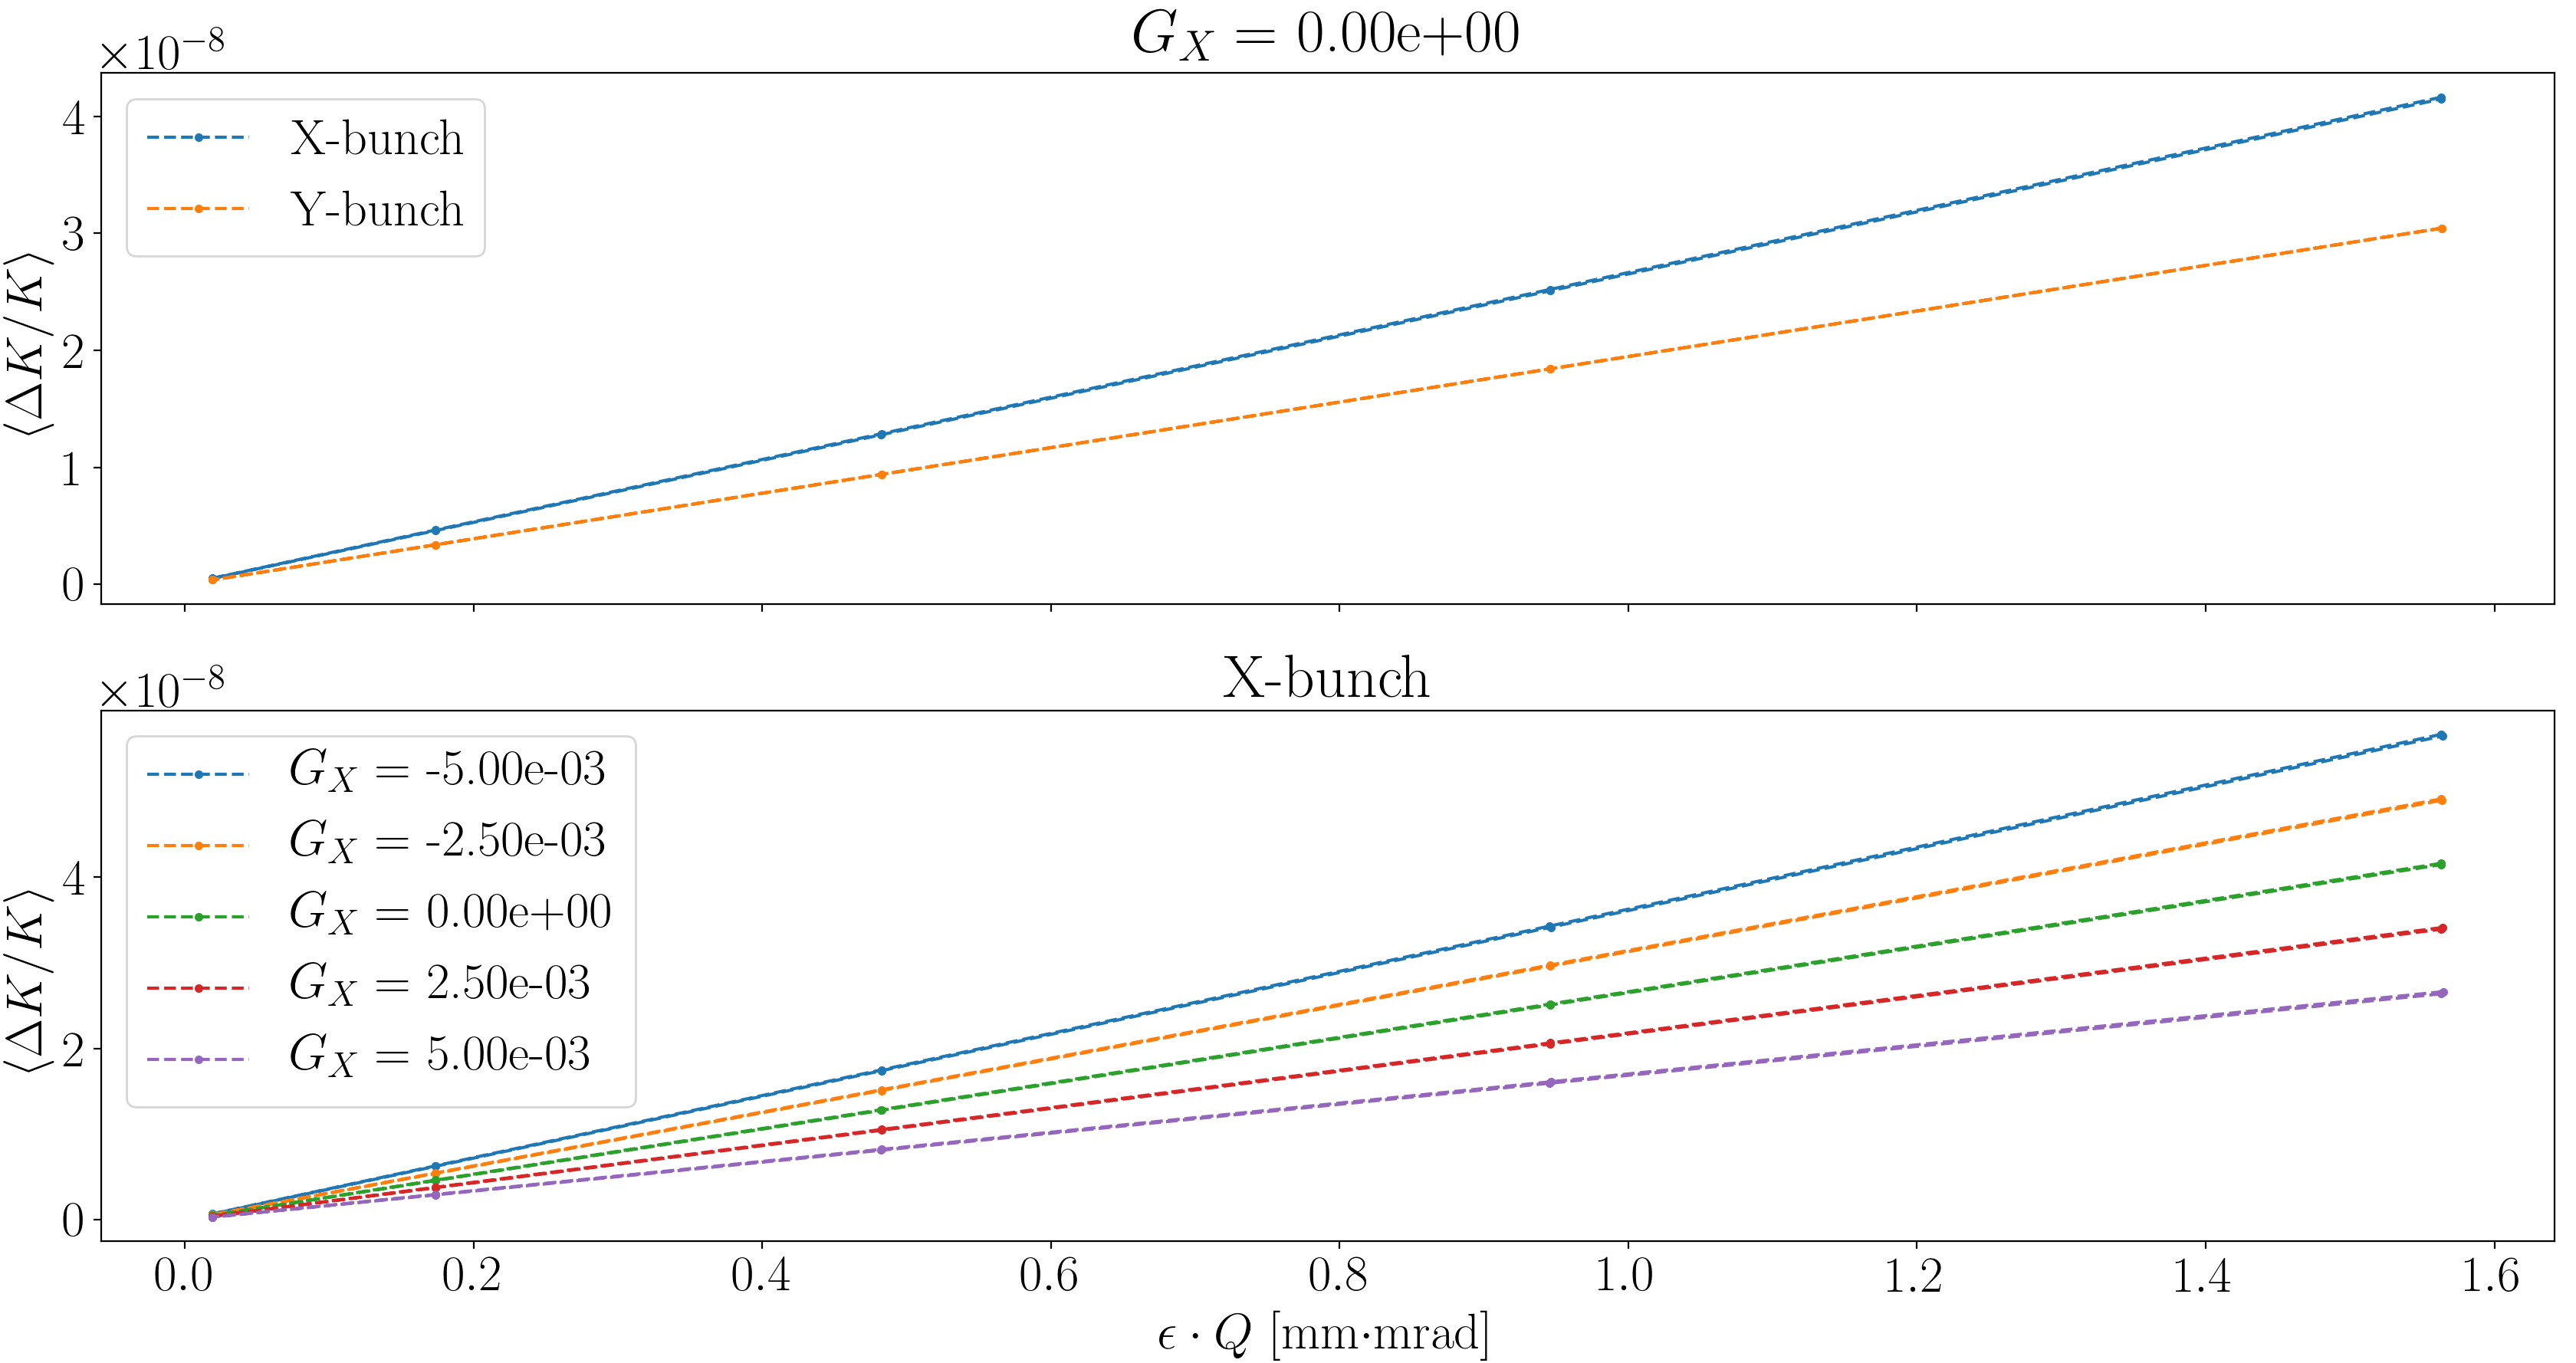
\includegraphics[height=.3\paperheight]{images/stune_traj_equ/part1/equ_energy_vs_emittance}
	\caption{Зависимость равновесного уровня энергии частицы от её поперечного эмиттанса.\label{fig:equ_nrg_vs_emittance}}
\end{figure}

Пространственная зависимость коэффициента сжатия орбиты подтверждается уравнением~(15) работы~\cite{Senichev:IPAC13}, в которой обнаруживаем:
\[
\alpha_0 = \avg{\frac{D_0}{\rho}},~~ \alpha_1 = \avg{\frac{D_1}{\rho}} + \frac12\avg{D_0'^2},
\]
где $D(s) = D_0(s) + D_1(s)\cdot \delta$  есть функция дисперсии, а $\rho$ --- радиус замкнутой орбиты частицы.
В первом приближении, дисперсия существует только в горизонтальной плоскости, и равна нулю в вертикальной. Таким образом, пространственная зависимость функции дисперсии находит отражение в пространственной зависимости коэффициента сжатия орбиты.

Для сравнения, результаты тех же тестов в случае линейных спин- и орбитальной трансфер матриц представлены на Рисунках~\ref{fig:stune_traj_equ_linear:stune_vs_nrg}, и~\ref{fig:stune_traj_equ_linear:nrg_vs_emittance}.  Как видно на Рисунке~\ref{fig:stune_traj_equ_linear:nrg_vs_emittance}, у всех частиц, совершающих бетатронные колебания в вертикальной плоскости, один и тот же уровень равновесной энергии, что свидетельствует о равенстве их замкнутых орбит, что в свою очередь говорит об отсутствии дисперсии в вертикальной плоскости. При этом, из Рисунка~\ref{fig:stune_traj_equ_linear:stune_vs_nrg} следует, что спин-тюн всех этих частиц одинаков.

\begin{figure}[H]
	\centering
	\subbottom[Зависимость среднего уровня энергии от поперечного эмиттанса частицы.\label{fig:stune_traj_equ_linear:nrg_vs_emittance}]{%
		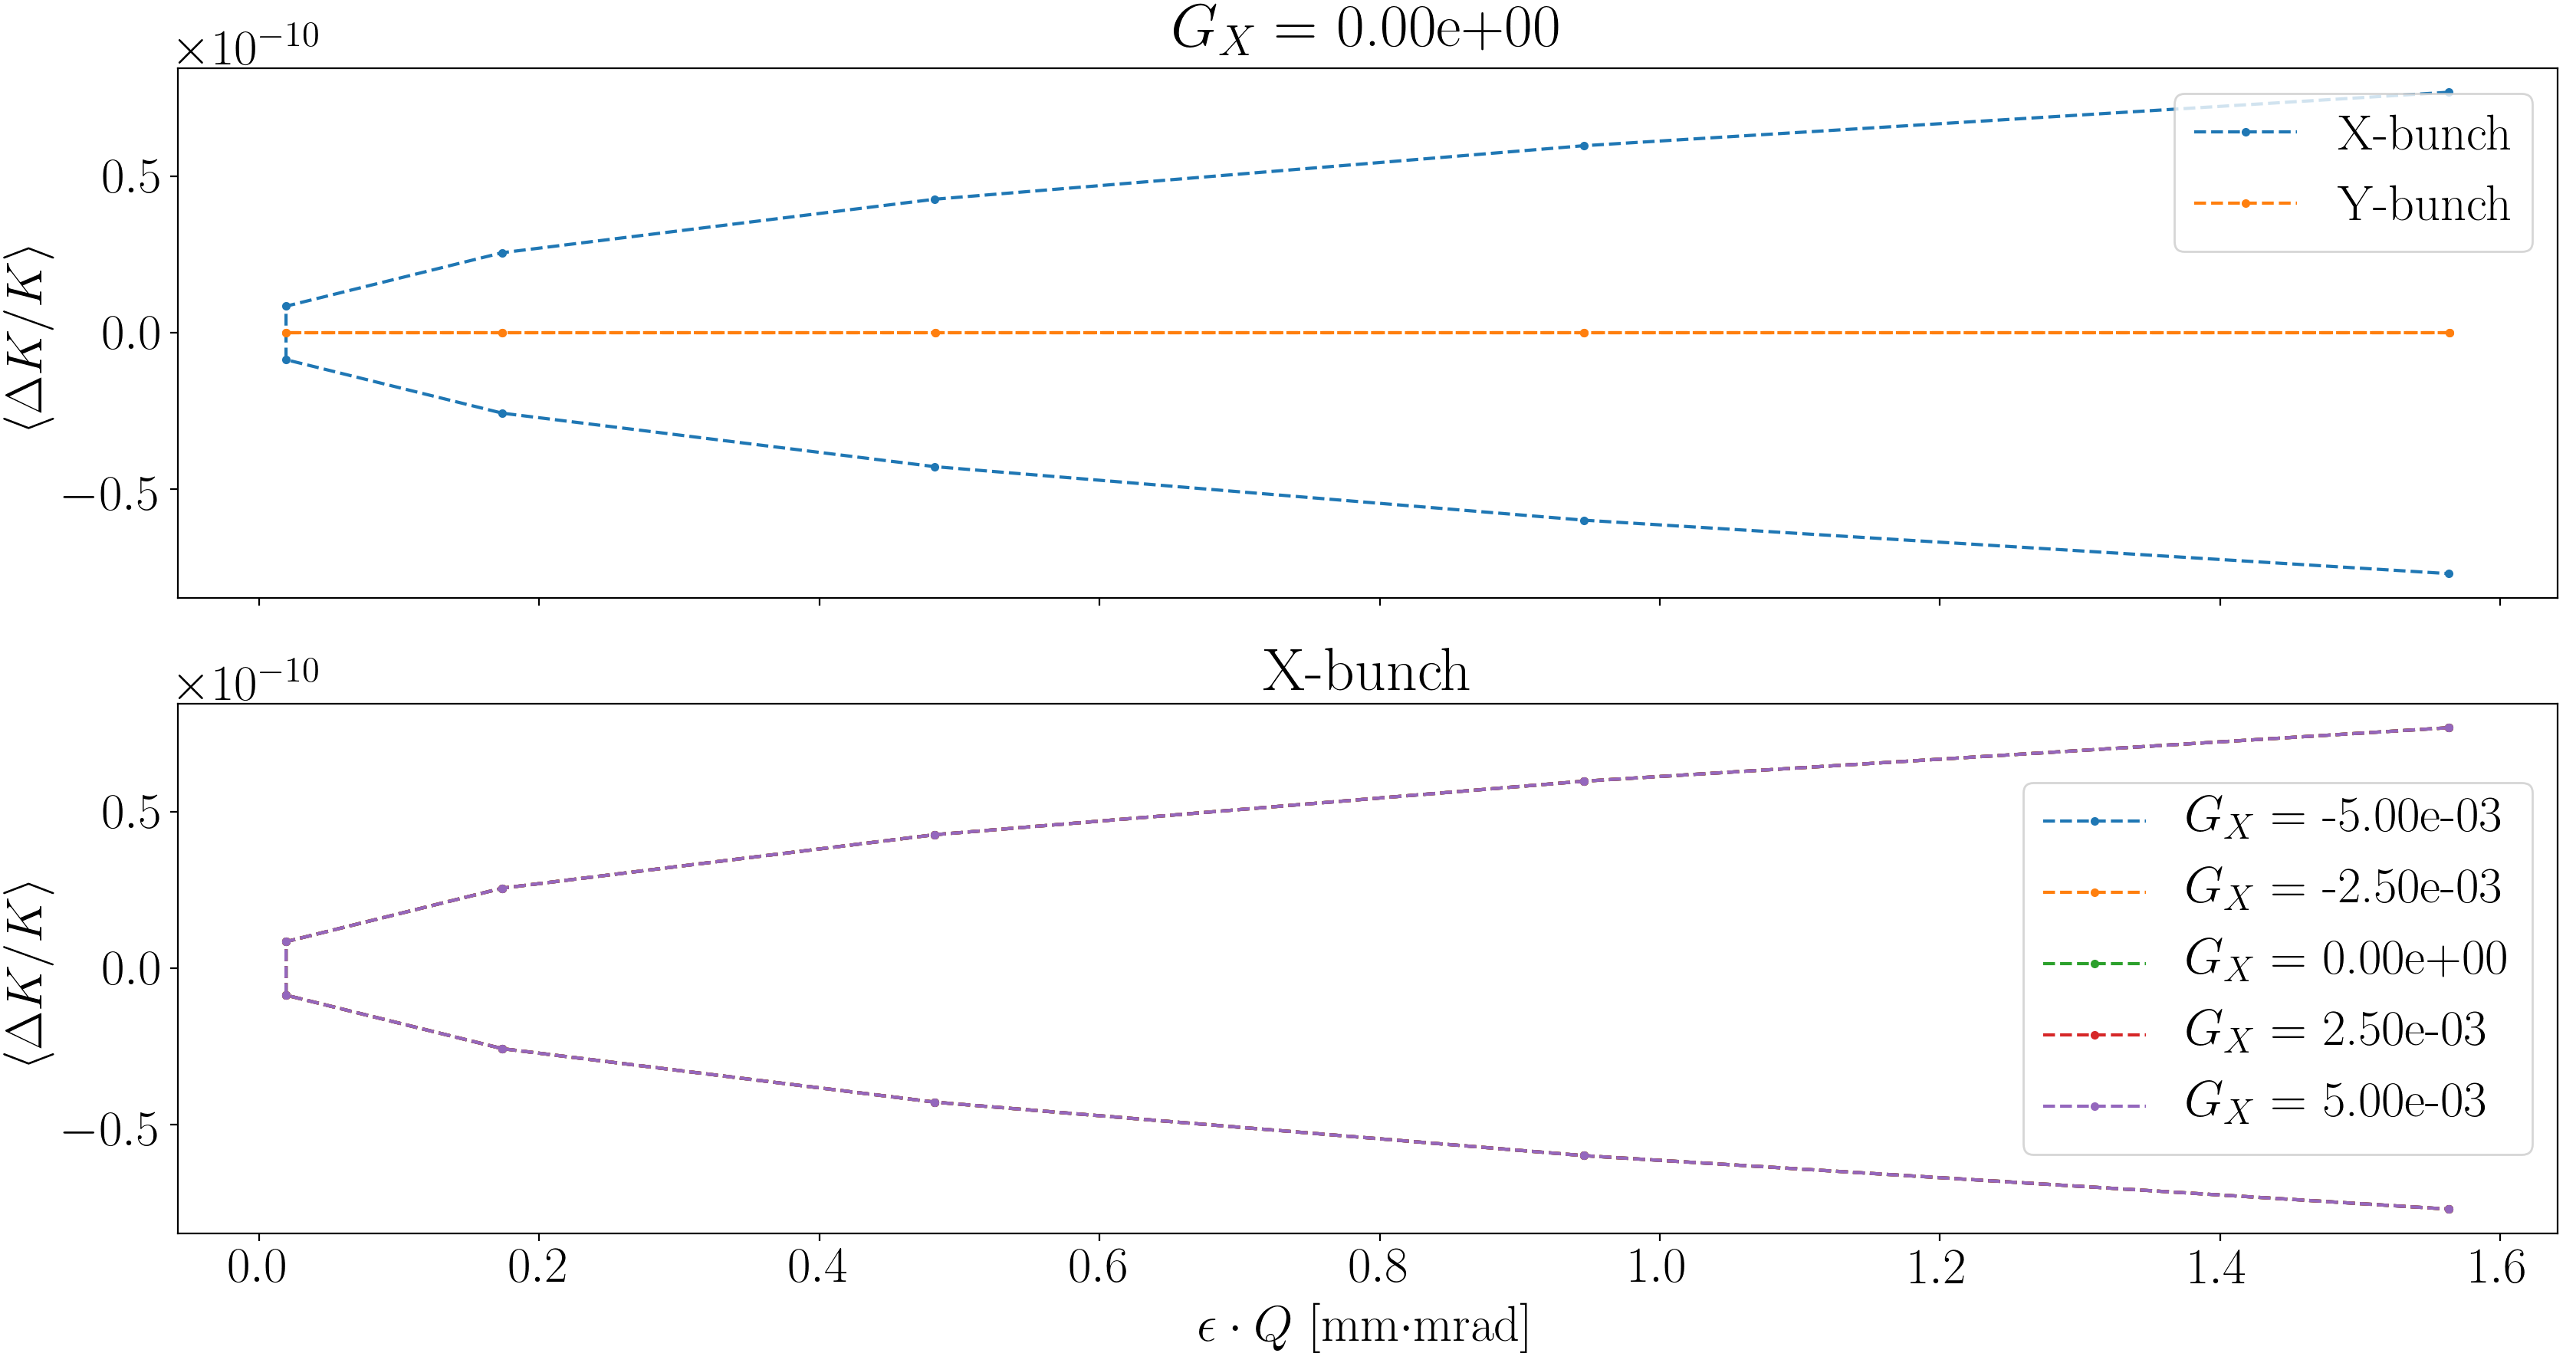
\includegraphics[width=\linewidth]{images/stune_traj_equ/part1/equ_energy_vs_emittance_linear}
	}
	\subbottom[Зависимость среднего уровня спин-тюна от среднего уровня энергии.\label{fig:stune_traj_equ_linear:stune_vs_nrg}]{%
		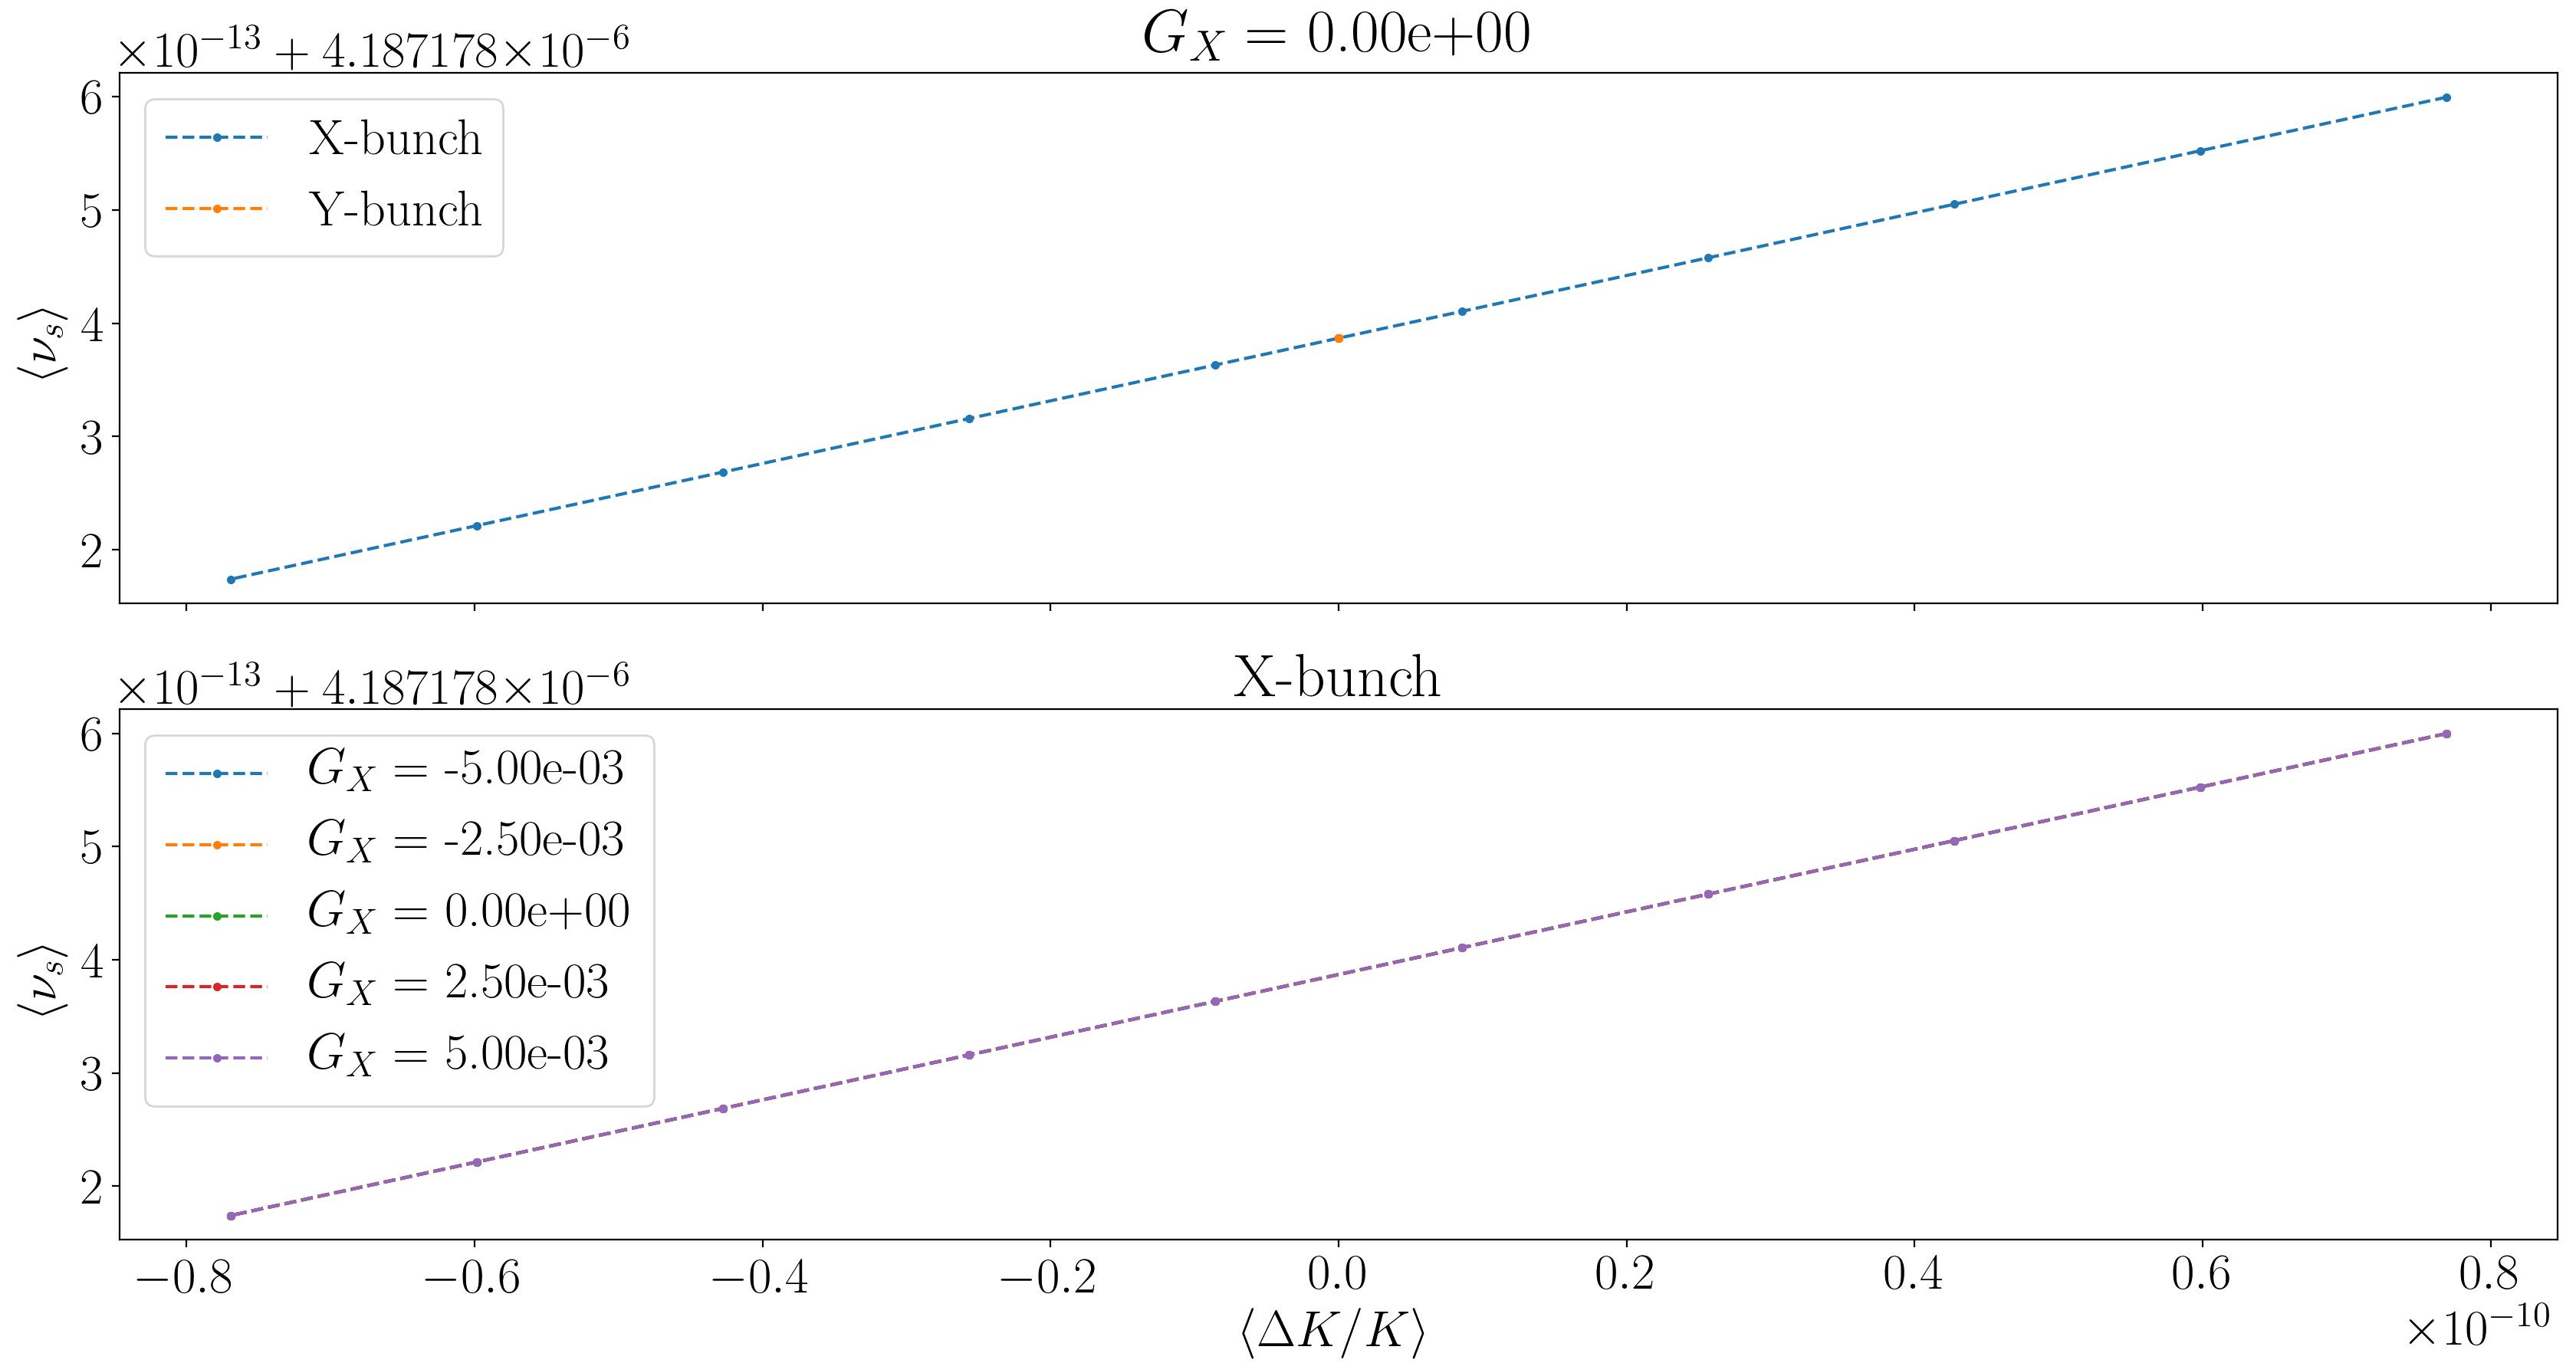
\includegraphics[width=\linewidth]{images/stune_traj_equ/part1/stune_vs_equ_energy_linear}
	}
	\caption{Результаты симуляции в случае линейного разложения трансфер матриц.}
\end{figure}

На Рисунке~\ref{fig:long_emitt_vs_trans_emitt} изображены зависимости продольных эмиттансов частиц от их поперечных эмиттансов (отнормированных бетатронными тюнами). Как видим, поперечные эмиттансы индуцируют продольные эмиттансы с разной скоростью, в зависимости от плоскости бетатронных колебаний частицы. В линейном случае, бетатронные колебания в вертикальной плоскости не индуцируют синхротронные колебания вовсе.
\begin{figure}[H]
	\centering
	\subbottom[Нелинейные разложения трансфер-матриц.]{%
		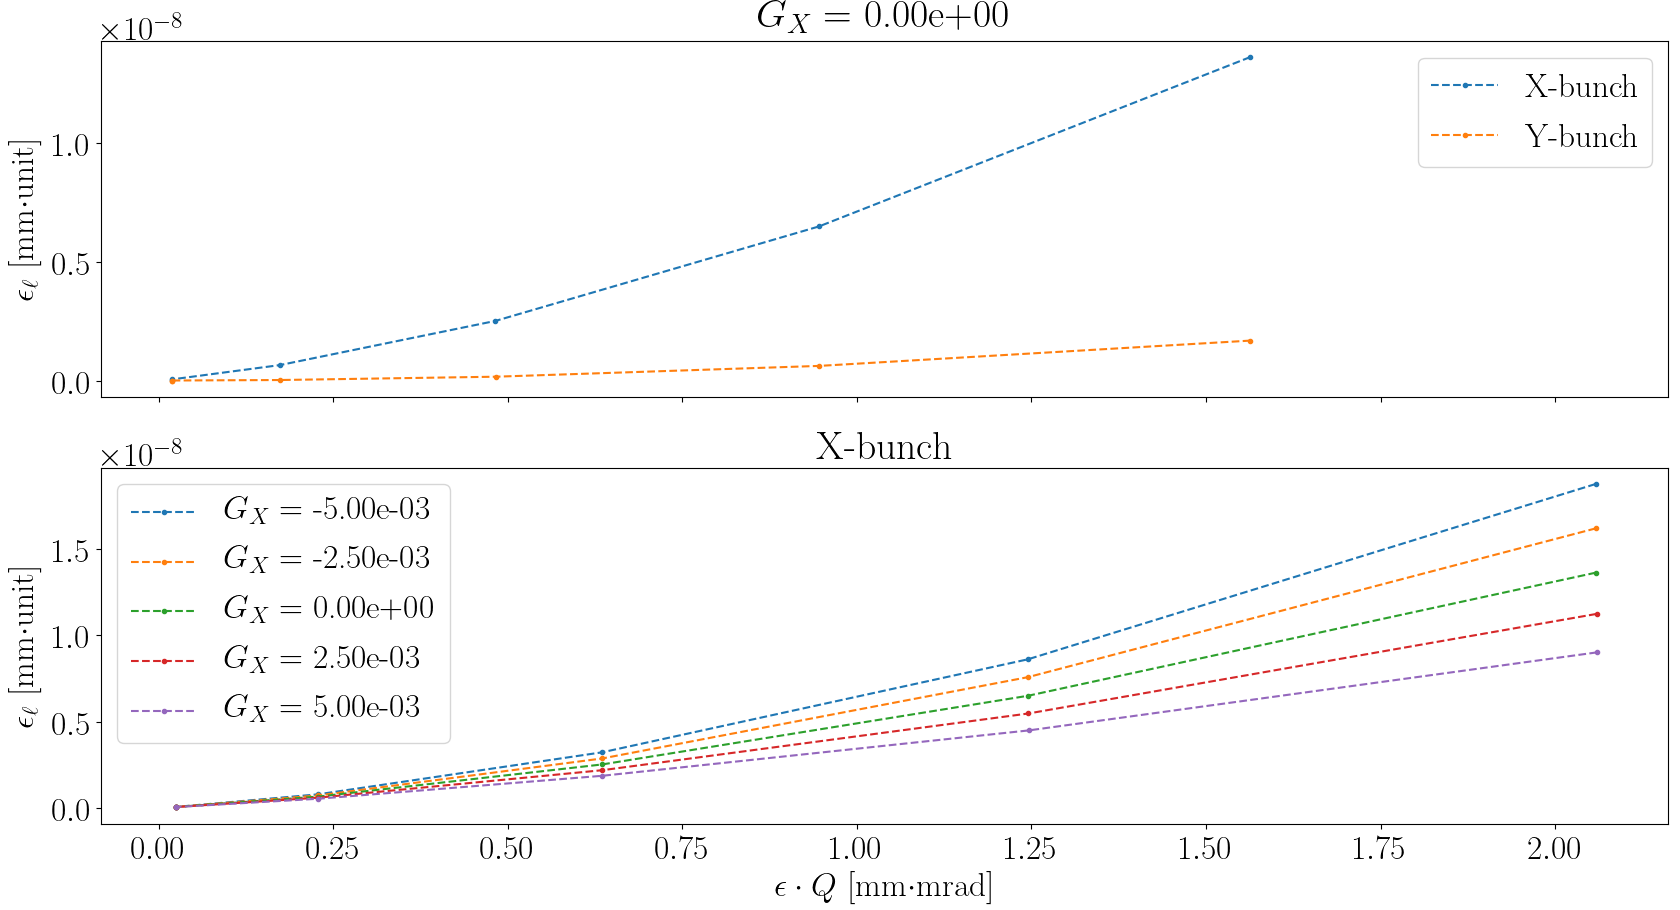
\includegraphics[height=.3\paperheight]{images/stune_traj_equ/part1/long_emitt_vs_trans_emitt}
	}
	\subbottom[Линейные разложения трансфер-матриц.]{%
		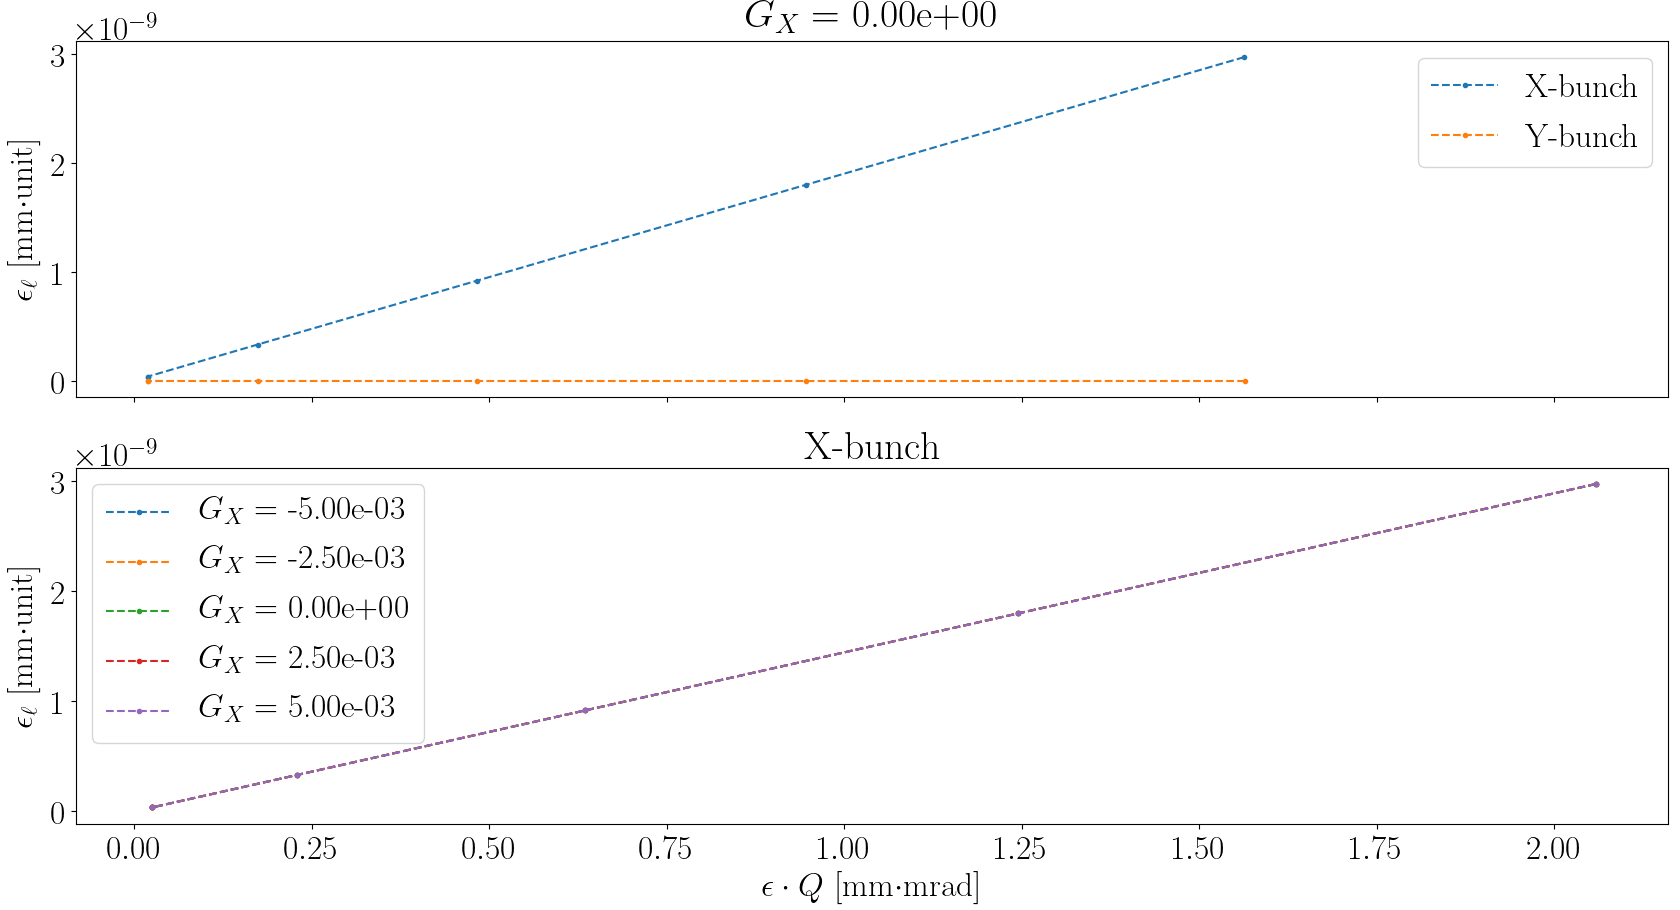
\includegraphics[height=.3\paperheight]{images/stune_traj_equ/part1/long_emitt_vs_trans_emitt_linear}
	}
	\caption{Зависимость продольного эмиттанса пучка от его поперечного эмиттанса.\label{fig:long_emitt_vs_trans_emitt}}
\end{figure}

\paragraph{Вывод:} Формулировка A не верна. 


\subsection{Формулировка Б}\label{sec:spin_stune_traj_equ:B_form}
\newcommand{\Ps}{\mathcal P}

При помощи кода COSY Infinity мы вычисляем функцию спин-тюна $\nu_s(\vec z)$ в виде
разложения ряда Тэйлора, где
\begin{align*}
  \vec z &= (x,a,y,b,\ell,\delta), \\
  \ell &= -(t - t_0)v_0\frac{\gamma-1}{\gamma}, \\
  \delta &= \frac{\Delta K}{K}.
\end{align*}

В настоящем разделе, проверим утверждение 1 в обобщённой форме B: функцию многих переменных $\nu_s(\vec z)$
можно представить в виде функции скалярного параметра $\nu_s(\g*)$; при этом, мы не будем предполагать
никакого формального выражения параметра $\g*$.

Если формулировка B верна, то существует система координат (одной из осей которых является $\nu_s$),
в которой частицы, совершающие бетатронные колебания в горизонтальной плоскости, неотличимы,
с точки зрения спин-тюна, от частиц, совершающих колебания в вертикальной плоскости. К тому же, в этой системе координат не должны присутствовать координаты из поперечного
фазового пространства $(x,a)$, и $(y,b)$.

Таким образом, будем рассматривать пространство $\Ps=(\ell, \delta, \nu_s)$. Если формулировка B верна,
различие траекторий частиц в поперечном фазовом пространстве не должно отражаться на траектории частиц в $\Ps$.

В анализе использованы данные симуляции, описанной в предыдущем разделе.

На Рисунке~\ref{fig:main:all_ps} изображена зависимость $\nu_s(\vec z)$ от $(\ell, \delta)$ в том случае, когда
$\vec z$ представляет реальную фазовую координату частицы в ускорителе. Мы наблюдаем:
\begin{enumerate}
\item стратификацию среднего уровня спин-тюна, как мы это видели в симуляциях по подавлению декогеренции
  в разделе~\ref{sec:decoh:sim-imperfect};
  \item стратификация гораздо значительнее для X-банча (синие точки), чем для Y-банча (красные точки).
\end{enumerate}

Последнее объясняется большим значением функции дисперсии в горизонтальной плоскости. Отметим, что при одинаковом приведённом поперечном эмиттансе~\footnote{Приведённым эмиттансом будем называть произведение $\epsilon_\alpha\cdot Q_\alpha$, где $\alpha\in\{x,y\}$.} (то есть одинаковом удлинении орбит, если исходить из уравнения~\eqref{eq:betatron_OL}), частицы, совершающие бетатронные колебания в горизонтальной плоскости, обладают значительно большим продольным эмиттансом, чем совершающие колебания в вертикальной плоскости.

\begin{figure}[h]
  \centering
  \subbottom[Подобраны траектории с равными приведёнными \emph{поперечными} эмиттансами.\label{fig:main:all_ps}]{%
    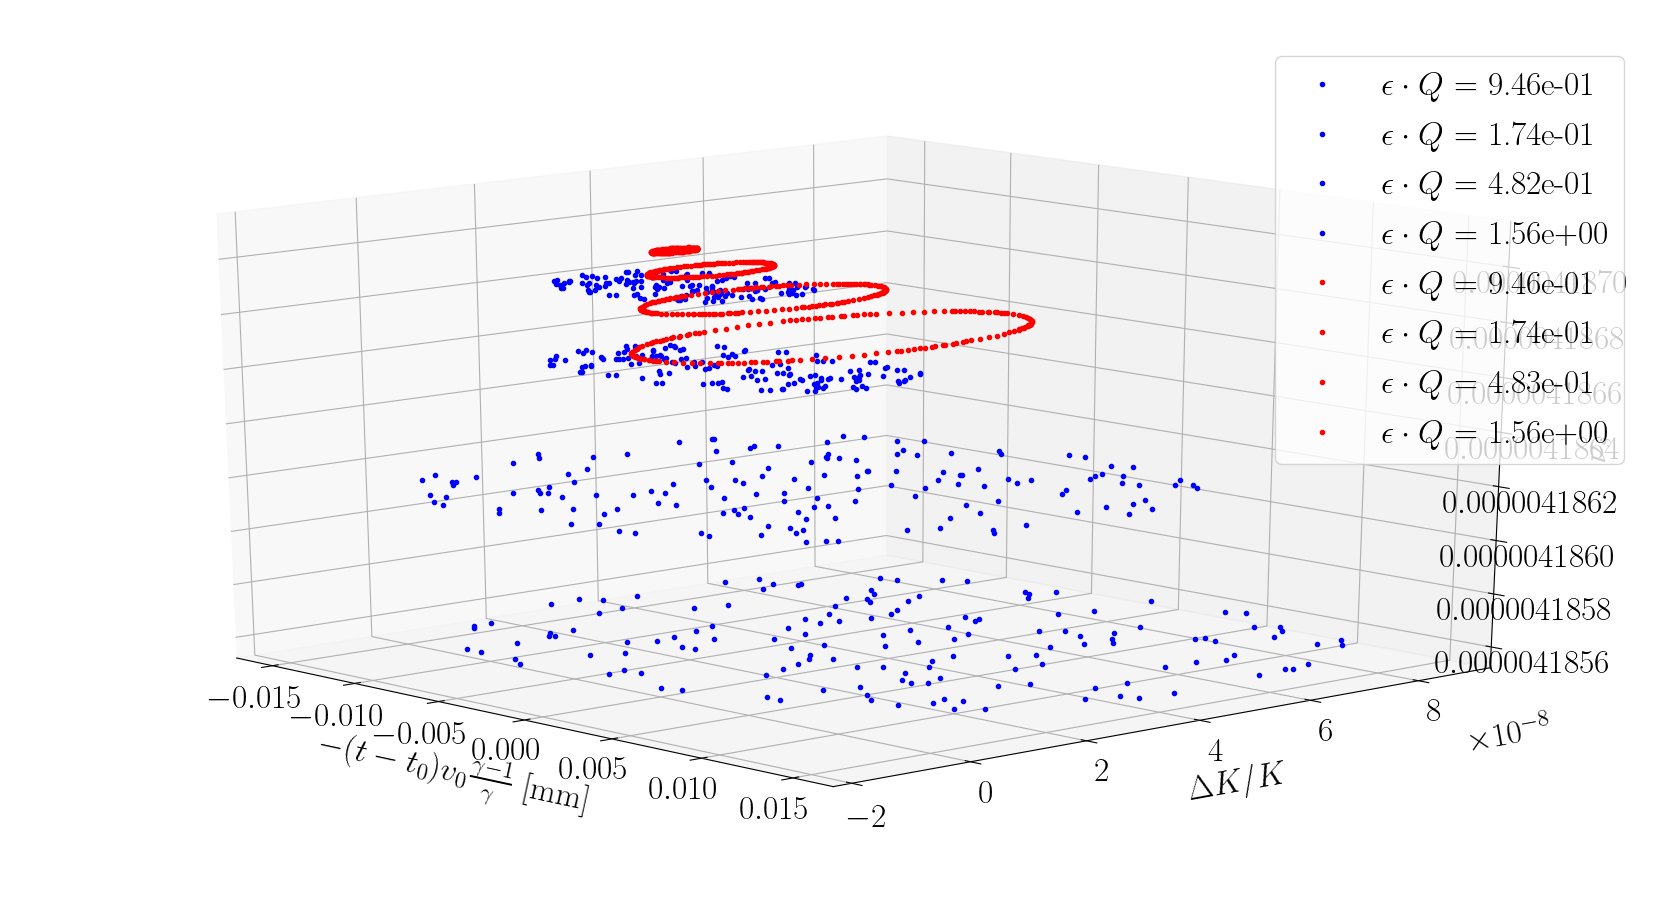
\includegraphics[height=.3\paperheight]{images/stune_traj_equ/part2/3D_plot_all_ps_vars}
    }
  \subbottom[Подобраны траектории с приблизительно равными \emph{продольными} эмиттансами.\label{fig:main:gamma_eff}]{%
    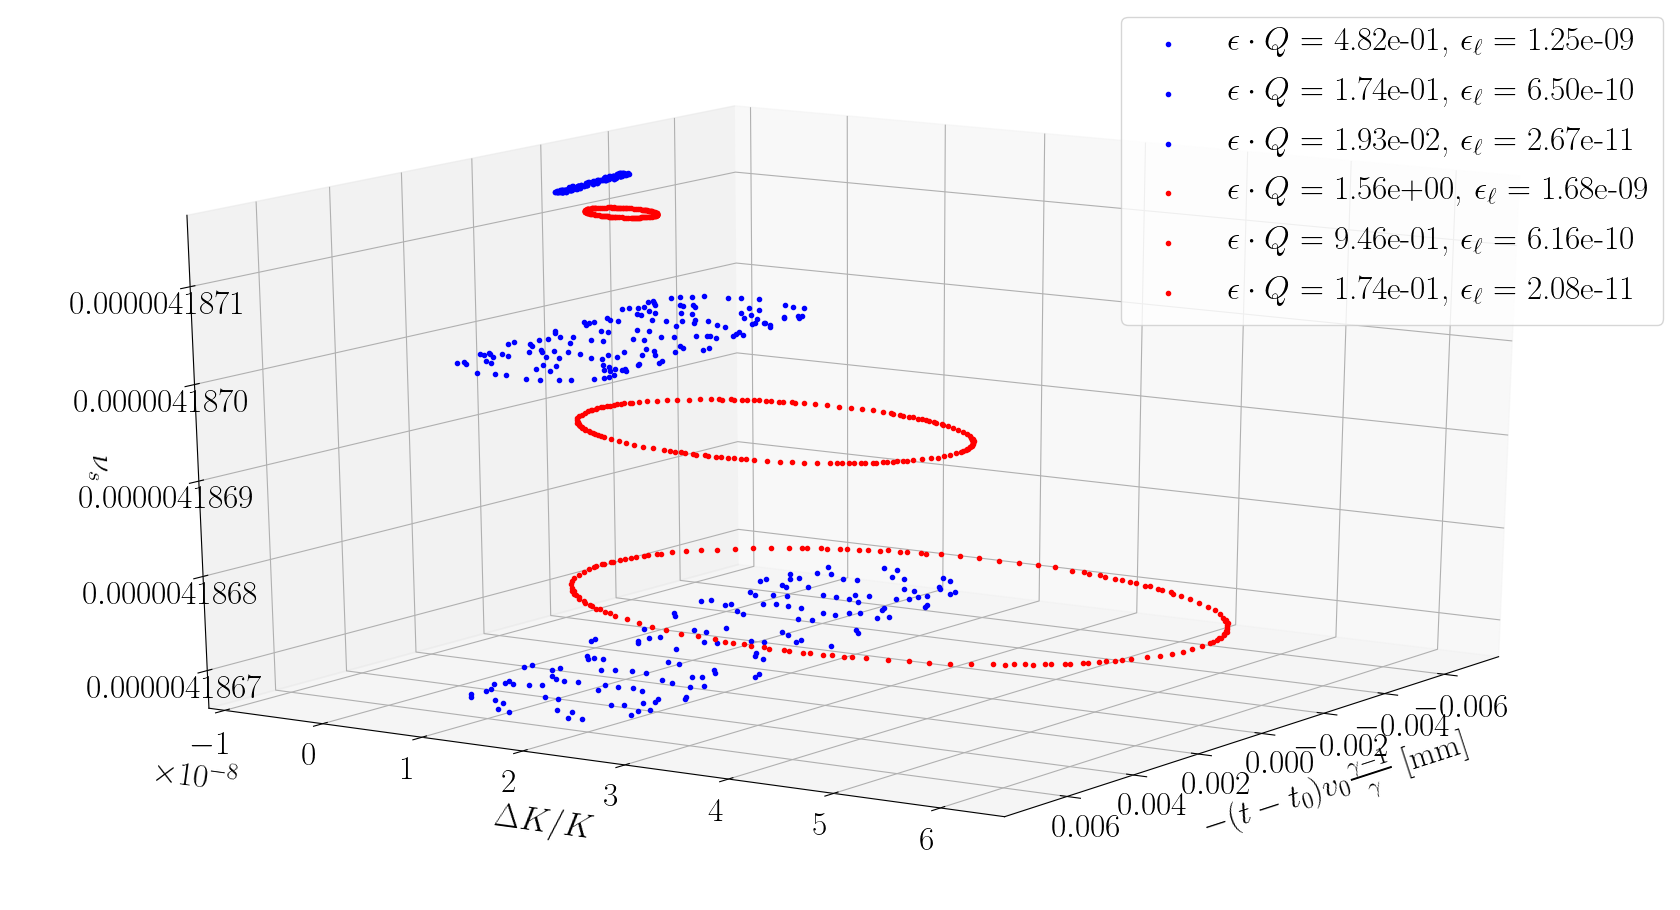
\includegraphics[height=.3\paperheight]{images/stune_traj_equ/part2/3D_plot_all_ps_vars_equal_long_emi}
    }
	\legend{Цветом обозначены частицы из разных банчей. Синий: из X-банча; красный: из Y-банча. В легенде указаны значения соответствующего банчу приведённого поперечного эмиттанса ($\epsilon\cdot Q$), и значение продольного эмиттанса ($\epsilon_\ell$) частицы.}
  \caption{Зависимость спин-тюна частицы от её положения в продольном фазовом пространстве.\label{fig:main}}
\end{figure}

В связи с последним, мы решили построить ту же самую зависимость, но подбирать пары частиц на основе равенства не приведённых поперечных эмиттансов, а на продольных эмиттансов. На Рисунке~\ref{fig:main:gamma_eff} мы наблюдаем, что частицы, с приблизительно одинаковыми продольными эмиттансами имеют приблизительно одинаковый уровень спин-тюна, независимо от плоскости совершения бетатронных колебаний.

\paragraph{Вывод:} формулировка B подтверждается симуляцией; эффективный Лоренц-фактор отражает величину продольного эмиттанса частицы.


\clearpage
